%\documentclass[12pt,a4j]{jreport}
\documentclass[a4paper,12pt]{jreport}
%\usepackage[dvips]{graphicx,color}
%\usepackage{array}main
%\usepackage{amsmath,amsthm,amssymb}
%\usepackage{refcheck}
%%%%%%%%%%%%%%%%%%%%%%%%%%%%%%%%%%%%%%%%%%%%%%%%%%%%%%%%%%%%%%%%%%%%
\usepackage[dvipdfmx]{graphicx}
\usepackage{url}
%\usepackage{epsfig}
\usepackage[fleqn]{amsmath}
%\usepackage[varg]{txfonts}
\usepackage{float}
\usepackage{caption}
\usepackage{flushend}
\usepackage{subfig}

%excel2latex用に追加
\usepackage{multirow}
\usepackage{bigstrut}


%筑波大学のフォーマットからコピー
\usepackage{times} % use Times Font instead of Computer Modern
\setcounter{tocdepth}{3}
\setcounter{page}{-1}

\setlength{\oddsidemargin}{0.1in}
\setlength{\evensidemargin}{0.1in}
\setlength{\topmargin}{0.1in}
%\setlength{\textwidth}{6in}
\setlength{\textwidth}{35zw}
%\setlength{\textheight}{10.1in}
\setlength{\textheight}{34\baselineskip}
\addtolength{\textheight}{\topskip}
\setlength{\parskip}{1.4mm}
\setlength{\topsep}{0em}

%%%%%%%%%%%%%%%%%%%%%%%%%%%%%%%%%%%%
%% タイトル生成用パッケージ(重要)
%\usepackage{sie-jp-sjis}
\usepackage{sie-jp-utf}

%% タイトル
%% 【注意】タイトルの最後に\\ を入れるとエラーになります
\title{入出力データの順序情報に基づくブラックボックステスト手法に関する研究}
%\title{A study on the method of blackbox testing based on I/O data sequence}
%% 著者
\author{湯本剛}
%% 学位 (2012/11 追加)
%\degree{}
%% 指導教員
%\advisor{}

%% 専攻名 と 年月
%% 年月は必要に応じて書き替えてください。
%\majorfield{△△△△}\programfield{□□□□}
\yearandmonth{2018年 3月}
%%%%%%%%%%%%%%%%%%%%%%%%%%%%%%%%%%%%%%%%%%%%%%%%%%%%%%%%%%%%%%%%%%%%
\begin{document}
\maketitle
\thispagestyle{empty}
\newpage

\thispagestyle{empty}
\vspace*{20pt plus 1fil}
\parindent=1zw
\noindent
%%
%% 論文の概要(Abstract)
%%
\begin{center}
{\bf 概要}
\vspace{5mm}
\end{center}
本研究はブラックボックステストのテストケース抽出に抜け漏れやケース数が増 大する課題に対して,
テスト対象に対する入出力データの順序情報に基づいてテストケースを抽出する 手法を提案し,合理的に
テストケースを抽出することを成果とするものである.
%%%%%
\par
\vspace{0pt plus 1fil}
\newpage

\pagenumbering{roman} % I, II, III, IV
\tableofcontents
\listoffigures
%\listoftables

\pagebreak \setcounter{page}{1}
\pagenumbering{arabic} % 1,2,3

%%%%%%%%%%%%%%%%%%%%%%%
%%%%%%%%%%%%%%%%%%%%%%
\chapter{緒論}
ソフトウェア開発工程の中で,品質を確保する主要な活動として,ソフトウェアテストがある.
ソフトウェアテストでは,テスト結果の情報を分析してテスト対象となるソフトウェアの品質を可視化することができる.
品質を可視化するためには,十分なサンプルデータを得られるだけのテストケースを実行しなければならない.
ソフトウェアテストを十分に行うために求められるテストケースの数は,昨今のソフトウェアの複雑性と規模の急激な増大に伴い,増加の一途をたどっている.
ブラックボックステストの場合,ソフトウェアの規模とテストケース数の関係は,ファンクションポイント総計値の1.15乗から1.3乗となる\cite{jones1998estimating}.
開発プロジェクトのファンクションポイント総計値は1970年から2000年までの30年間で約10倍に増大している\cite{longstreet2000}.
組み込みソフトウェア開発のソフトウェア規模の増大は,ドメインによって毎年10パーセントから20パーセントに及ぶという調査結果もある \cite{jones2009}.

ソフトウェアの規模の増大に伴ったテストケース数の増加に対応するために必要となるテスト工数は,ソフトウェア開発工数の多くを占めるようになってきている.
日本におけるテスト工数の割合は開発工数全体の28パーセントから35パーセントを占めるケースが多いが,90パーセントを超えるケースもあるという調査結果が出ている\cite{IPA2015}.
昨今のソフトウェアの開発は,新規開発が減少傾向にあり,システム統合,派生開発\cite{simizu2005}\cite{simizu2009},保守開発,コンポーネントベース開発\cite{gao2003testing}といったすでに利用されているものに対して追加,改良をする開発が多くを占めてきている.
日本における新規開発の比率がエンタープライズシステム開発で51パーセント\cite{IPA2015},組み込みソフトウェア開発で5パーセント\cite{IPAE2015}だという調査結果からも新規開発の減少傾向が読みとれる.
ソフトウェア保守開発においては,開発対象のソフトウェアを分析し,理解するための工数が工数全体の40パーセントから60パーセント必要となる.しかし,現実的には,十分にその工数を確保できないことが課題だといわれている\cite{abran2004guide}.

また,この種類の開発は,テスト工数の比率が大きくなることが多い.
複数のシステムを統合するといった大規模な開発にて8ヶ月の間に約5000人がテスト工程に投入されたという事例もある\cite{MTBUDay2}.
これらの調査結果から,開発全体に占めるソフトウェアテストの割合が多いほど開発コストに与える影響も大きくなるといえる.
そのため,ソフトウェアテストを効率的に行うことが開発コストを左右すると考えられる.
効率のよいテストとは,テスト対象の品質を可視化するために使うリソースが少ないことである.

ソフトウェアテスト工程全体の中の活動のうち,テスト実行がソフトウェア開発のクリティカルパス上にある唯一の活動となる.
特に,開発の要件が期待通りに実現しているかを確認するシステムテストのレベルにてソフトウェアをテストする局面では,開発工程で作られるソフトウェアだけでなく,既存のソフトウェアや実行環境など,実運用で必要となるものがすべて合流する.ここでのテスト実行は,クリティカルパス上にある活動となる.
テスト実行がクリティカルパス上に滞在する期間をどの程度短くできるかが,開発コストだけでなく開発期間にも大きく影響を及ぼす.

テスト実行がクリティカルパス上に滞在する期間を短くする方法は,対象範囲を絞る\cite{rothermel2002empirical},欠陥の修正を効率化する\cite{matsuodani2004evaluation}などがあり,多くの研究がある\cite{beer2008role}\cite{weinberg2008perfect}.
その1つとして,テスト実行の開始よりも早い段階でテストケースを抽出し,テストすべき内容の全体を示すことがあげられる.
これにより,効率の良いテスト実行を計画できるためである.
テストケースを開発する活動が遅延して,テスト実行の活動を逼迫しないようにするためには,複数の人員を投入し,計画した期間内でテストケースを作る必要がある.
テストケースを開発する工数は,平均的にテスト工数全体の40パーセントだと言われている\cite{van2013tpi}.
この調査結果は,テストケースの開発には多くの人員が必要となることを示している.
昨今のソフトウェアの規模と複雑性の増大から,必要となるテストケース数はとても多くなり,数万から数十万となることも珍しくない.
前述した大規模なシステム統合プロジェクトの事例では,統合テストとシステムテストのテストケース合計が1,030,000ケースであったと報告されている.

多数の人員が大量のテストケースを抽出する活動に必要とされているにもかかわらず,テストケースを開発するための明確に定義されたルールがないことが多い.
そのために,投入された人員は個々の考え方に基づいてテストケースを開発することになる.
この方法は,ソフトウェア保守開発の課題と同様に,それぞれのテスト対象を分析し,理解した内容に一貫性がなく,対象範囲の整理が不十分なまま大量のテストケースが作られていくことを意味している.
ソフトウェアテストを十分に行うためには,重複が無く抜け漏れの無いテストケースを開発することが重要になる.
しかし,ソフトウェア規模の増大,また短納期のプレッシャーを受けながら,上記したように大量の人員で大量のテストケースを効率的に作らなければならないことは,以下の問題を引き起こす.
\begin{enumerate}
\item テストケースが重複する.同じテストを複数人が実行することになるため作業効率が低下する.
\item テストケースが欠落する.テスト実行に入ってからテストケース追加が必要になり作業効率が低下する.
\end{enumerate}

これらの問題は,コスト増や納期遅延の原因となるだけでなく,テストの活動がソフトウェアの品質を確保する役割を果たせなくなる問題となる
\cite{bertolino2007software}
\cite{mantyla2013more}
\cite{mantyla2014time}.

また,テスト対象の規模が大きくなるほど,複数の機能を組み合わせたテストケースを実行する必要が出てくる.
機能の組み合わせを単純なルールで網羅するようにテストケースを抽出すると,テストケース数が乗算で増えてしまうため,テストケースを増やさない工夫が必要となる.
そのためには,対象を理解し,目的に沿ったテストだけを行うことが重要である\cite{kaner2008lessons}.
投入された多くの人員がテストケースを増やさないように目的に沿ったテストケースだけを作るためには,目的に沿った網羅基準と適切な抽出方法が必要である.

本研究では,テストケースを開発する活動に携わる人員が,適切に対象を理解することで,必要なテストケースを網羅的に抽出し,抜け漏れを防止できるようにすることを目的とする.
テストケースを開発する対象として,システムテストレベルでのブラックボックステストに着目する.
テストレベルの中でもシステムテストは,開発の規模に伴い規模が大きくなり,それに伴いテストケースの開発にも多くの人員が投入されることになるためである.
そして,システムテストのレベルでのテスト対象への入出力データの順序情報を分析し,適切な数のテストケースを開発するための手法を提案し,手法の適用評価を行う.

本論文は6章で構成される.
2章では,システムテストのレベルでのブラックボックステストにおける課題と,関連する先行研究について述べる.
また,本研究のベースとなるテスト分析手法であるテストカテゴリベースドテストの概念,作業ステップ,そして適用時の効果を調査した実験結果を述べる.

3章では,前章で述べた課題を更に分析するためにおこなった実験の結果を述べる.
実験は3回行なった.
3回の実験から,テストケースの抽出結果には,ばらつきがあること,また,手法を取り入れることによって漏れていたテストケースが抽出できるようになることを確認する.
また,実験結果から読み取れる傾向を考察する.

4章では,システムテストレベルにて,テストを実行する際の入出力データに着目する.
テスト実行はデータの入出力を行うことであり,この全体像をI/Oテストデータパターンとして定義し,このパターンを網羅することでテスト対象の分析を網羅的に行うことができる.
このI/Oテストデータパターンを適用した分析手法を提案する.
I/Oテストデータパターンの適用評価では,現実のプロジェクトで実際に使用されたテストケースと,提案する手法で作ったテストケースを比較し,現実のプロジェクトにてどのようなテストケースが不足するのかを考察する.

5章では,入出力の実施順序から重要な順序組み合わせを抽出してテストケースにする方法として,テスト実行時のデータフローに着目する.
複数の機能の統合を確認するためには,複数回のテストデータの入出力が必要となる,
統合は多くの機能を組み合わせていくため,2回以上のテストデータの入出力を組み合わせる必要も出てくる.
テストデータの入出力を順番に組み合わせる必要がある際に,単純に2回のテストデータ入出力の組み合わせ,それ以上の回数の入出力の組み合わせを洗い出してテスト実行順序を網羅しようとすると,実行順序の組み合わせ数を乗算で求めるようになるため,テストケース数が爆発する.
そこで,機能間の統合を確認するためのテストケースを抽出するために,データフローに関する設計文書をベースに順序組み合わせを抽出する方法である順序組み合わせテストとその網羅基準である波及全使用法(Impact Data All Used:IDAU)を提案する.
この適用評価では,順序組み合わせテストを使って実在の仕様書,設計書からテストケースが抽出できることの実証行う.
また,順序組み合わせのテストケースを抽出する既存の手法である状態遷移テストを比較し,テストケース抽出内容を考察する.

最後の6章では,これらの研究をまとめて,結論を述べる.

%%%%%%%%%%%%%%%%%%%%%%%
%%%%%%%%%%%%%%%%%%%%%%%
\chapter{システムテストにおけるブラックボックステストの課題}
本研究は,アプリケーションソフトウェアを開発する際に行うソフトウェアテストの中で,システムテストレベルでのブラックボックステストを研究対象にする.ブラックボックステストのテストケースを開発するプロセスの中では,テスト分析を対象にする.
本章では,これら研究対象の範囲を明確にするために定義を説明し,そこで起きている課題を述べる.
また,この研究のベースになるテスト分析手法である,テストカテゴリベースドテストについて説明する.

\newpage
\section{テストケースの開発方法とテストレベル}
\subsection{アプリケーションソフトウェアの構成}
本研究では,図\ref{fig:fig-1}に示す状態$St$と保持データ$Ds$を持つアプリケーションソフトウェア$AS$に対するソフトウェアテストを研究対象にする.アプリケーションソフトウェア$AS$は,入力$In$に対して,何らかの出力$Out$を返す.
ソフトウェアの機能は,何らかの入力$In$を出力$Out$に変換する処理により実現されていると考えられる.
この処理を本研究ではタスク$Ta$と呼ぶ\cite{yumoto2017ICST}.
タスク$Ta$は,該当のテストレベルからみた入力を出力に変換している1処理である.
そのため,タスク$Ta$のサイズは,テストレベルによって決まる.
ユニットテストのレベルであれば関数となり,システムテストのレベルであれば,システムを利用するユーザが操作する機能となる.
ソフトウェアの構成要素であるタスク$Ta$の出力$Out$について考えると,$Ta$への入力$In$だけでなく状態$St$と保持データ(データベースや内部メモリに保存されているデータ)$Ds$の影響を受けると考えられる.
たとえば,Webアプリケーションにて予約を行うタスク$Ta$について考えると,予約が可能か否かを示す状態$St$と,予約オブジェクトの予約状況を示す保持データ$Ds$によって予約の成否が決まる.

%−−−-図1を入れる
\begin{figure}[H]
  \begin{center}
  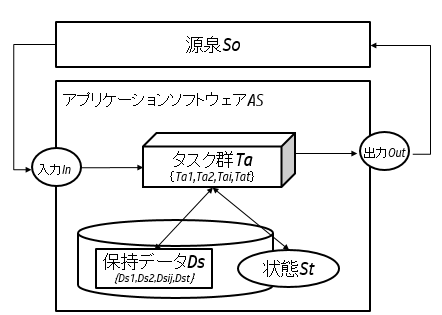
\includegraphics[width=11cm]{./image/fig-1.png}
  \caption{アプリケーションソフトウェアの構成}
  \label{fig:fig-1}
  \end{center}
\end{figure}

アプリケーションソフトウェア$AS$の構成要素は,タスク群$Ta$と状態$St$と保持データ$Ds$とし,外部の源泉$So$からの入力$In$と$So$への出力$Out$があるとする.
タスク群$Ta$は,その要素を$Ta=\{Ta_1,Ta_2,\cdots,Ta_i,\cdots,Ta_t \}$とし, 対応する入出力は$In_i$と$Out_i$とする.
\subsection{ホワイトボックステストとブラックボックステスト}
テストケースの種類は,ソフトウェアの物理的な構造をベースにテストケースを抽出するホワイトボックステストと,ソフトウェアの仕様をベースにテストケースを抽出するブラックボックステストに大別できる\cite{myers2011art} .

\begin{figure}[htbp]
  \begin{center}
  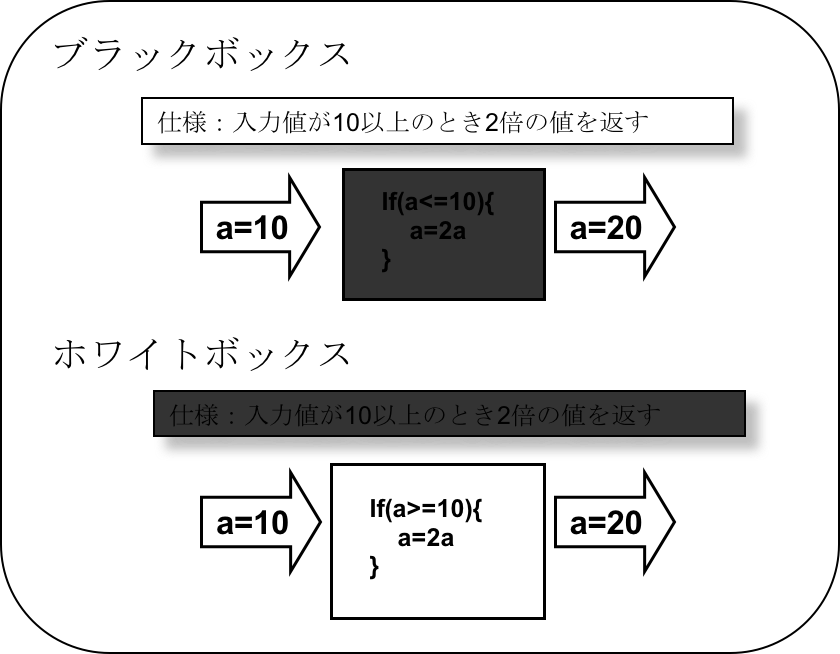
\includegraphics[width=10cm]{./image/D-2-BbWb.png}
  \caption{ホワイトボックステストとブラックボックステストの違い}
  \label{fig:D-2-BbWb}
  \end{center}
\end{figure}

ホワイトボックステストとブラックボックステストの違いを図~\ref{fig:D-2-BbWb}に示す.
両者の違いはテストの網羅基準とテストケースの抽出方法の違いである.
ホワイトボックステストは,テストケース抽出のベースがテスト対象となる$AS$の内部要素である$Ta$の構造になる.
ユニットテストのレベルで例えると,$Ta$の内部構造となるプログラムのソースコードの行を網羅,分岐を網羅するように$In$を与えて$Out$を確認するといったように,網羅すべきアイテムを明確に選択してテストケースを開発する.
網羅基準はテスト設計技法として提唱されている\cite{beiz90}
\cite{tj2005}
\cite{lewis2016software}
\cite{ammann2016introduction}
\cite{copeland2004practitioner}.

一方,ブラックボックステストは,テスト対象そのものではなく,$Ta$に対する動作条件や振る舞いについて記述した仕様をベースにしてテストケースを開発する.
ブラックボックステストのテスト設計技法では,仕様に対する網羅基準が数多く提唱されている\cite{jorgensen2016software}
\cite{binder2000testing}
\cite{kaner1999testing}
\cite{black2007pragmatic}
\cite{Ostrand:1988:CMS:62959.62964}
\cite{Grindal:2007:IPM:1332044.1332085}.

しかし,ブラックボックステストは,テストケース抽出のベースがテスト対象の物理的な構造ではなく論理的なふるまいの記述であるがゆえに,テストを作るための詳細化が複数の解釈で行われることが多い.
これに起因する課題については,2.2節にて述べる.

本研究では,テストケースの設計方法の種類は,ブラックボックステストを対象とする.

\subsection{テストレベル}

ソフトウェアテストは,開発ライフサイクルの中で複数のテストレベルに分けて行われる\cite{young2008software}.
複数のテストレベルは,図~\ref{fig:D-2-Fig1}で示すVモデルと呼ばれる技術面にフォーカスしたライフサイクルモデルにて表現することができる\cite{forsberg}.
テストレベルは,ソフトウェア開発の段階的詳細化のレベルと対応している\cite{pressman2005software}.

\begin{figure}[htbp]
  \begin{center}
  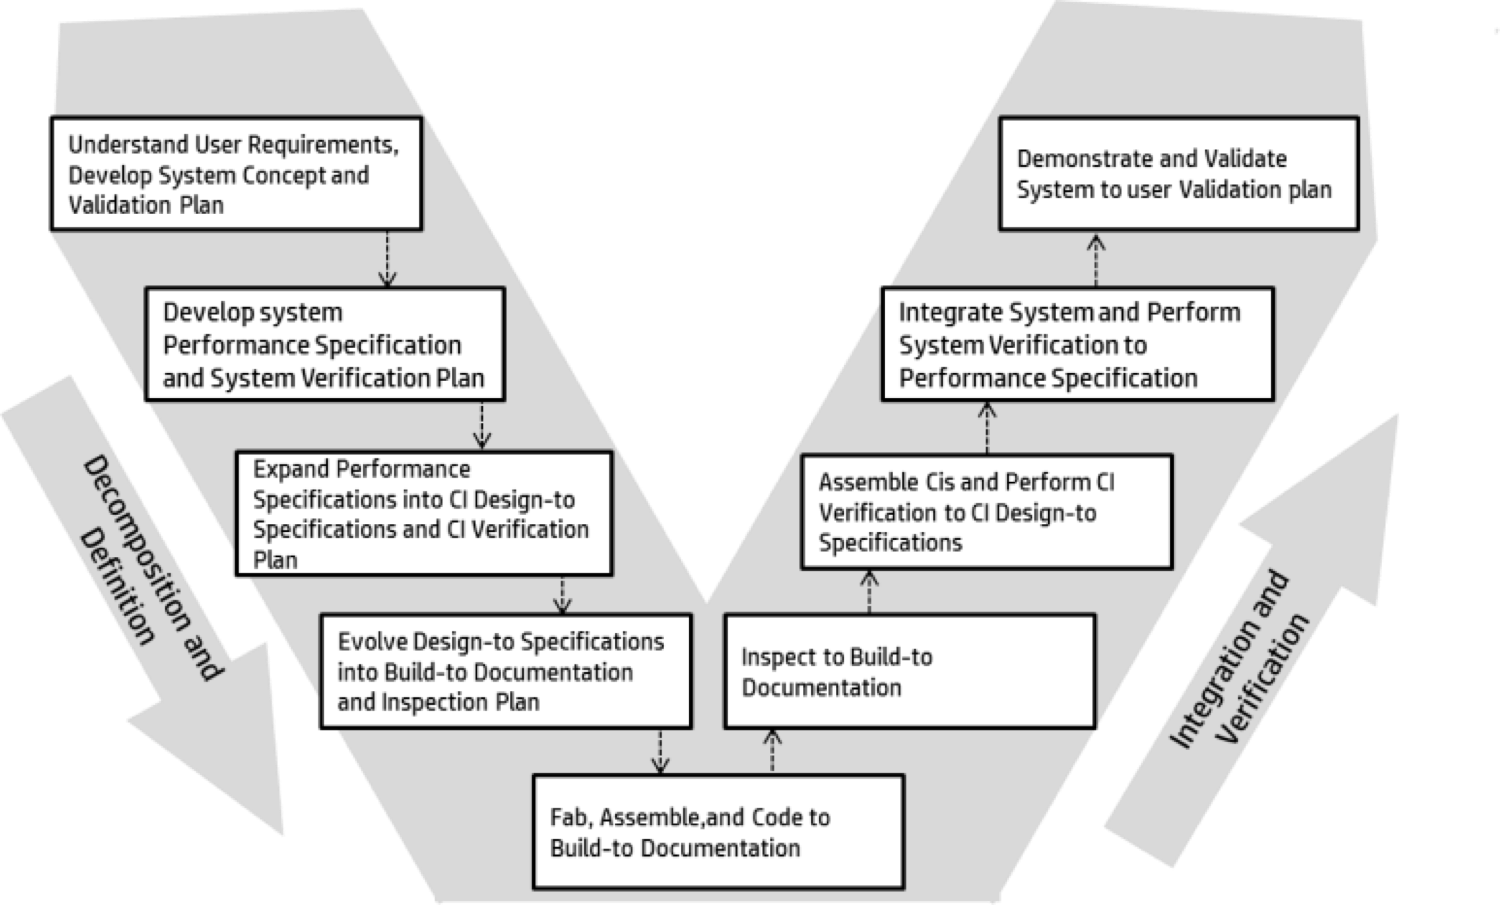
\includegraphics[width=12cm]{./image/D-2-Fig1.png}
  \caption{Vモデル}
  \label{fig:D-2-Fig1}
  \end{center}
\end{figure}

テストのプロセスは,Vモデルであらわす各レベルごとに行われる\cite{yumoto2006}.
本研究は,複数のテストレベルの中で,図~\ref{fig:D-2-Fig1}の上から2番目の箱となる,「Develop System performance specification and System verification plan」と「Integration system and Perform system verification to performance specificetion」のレベル,つまりシステムテストのレベルで実行するブラックボックステストに焦点を当てている.
システムテストのレベルは,開発した単体のソフトウェアがすべて統合されるため,規模と複雑性の増大による影響を直接的に受けるからである.

\subsection{テスト開発プロセス}
Vモデルであらわす各レベルにて行われるテストは,それぞれ開発プロセスと類似したプロセスを持っている.
テストのプロセスは, 図~\ref{fig:D-2-Fig2J}のようにテスト計画がVモデルの左側の活動と並行に行われ,その後時系列にテスト分析,テスト設計,テスト実装が行われた後,Vモデルの右側の活動の中で,テスト実行と終了基準の評価が行われる.
\begin{figure}[htbp]
  \begin{center}
  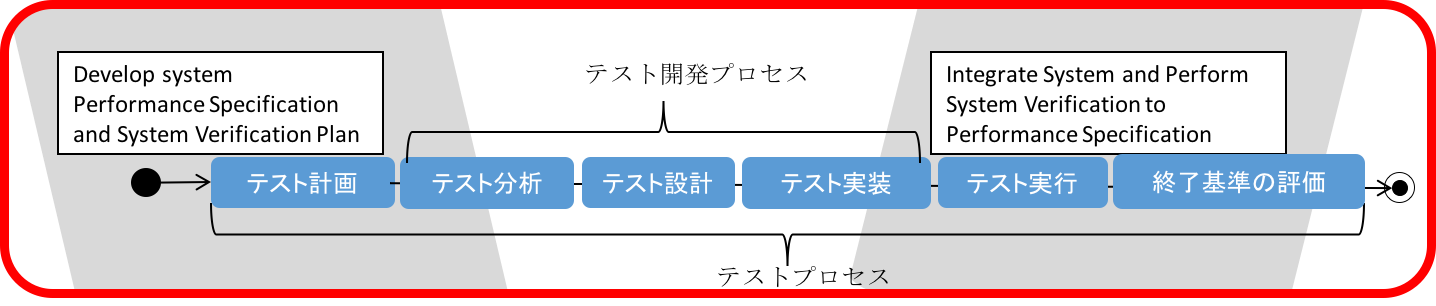
\includegraphics[width=14cm]{./image/D-2-Fig2J.png}
  \caption{テスト開発プロセス}
  \label{fig:D-2-Fig2J}
  \end{center}
\end{figure}
テストのプロセスの中でテスト分析,テスト設計,テスト実装の3つのテストケースを抽出するための活動はテスト開発プロセスと呼ばれている\cite{ISTQB}.

本研究では,テスト開発プロセスの中のテスト分析とテスト設計を対象とする.
テスト分析では,テストすべきアプリケーションソフトウェア$AS$をテスト設計ができるサイズに詳細化する.
ブラックボックステストでのテストケースを開発するベースは,対象とするアプリケーションソフトウェア$AS$の仕様である\cite{stocks1996framework}.
仕様とは,図~\ref{fig:D-2-Fig1}で示したVモデルの左側の成果物のことである.
各テストレベルにてテストケースを開発するベースとなる仕様をテストベースと呼ぶ\cite{craig2002systematic}.
本研究の対象となるテストレベルでは,Develop System performance specification and System verification planでの成果物がテストベースとなる.

テスト分析では,テストベースに記述された仕様から,テストすべき$AS$の動作条件や振る舞いを特定する.
仕様には,テストでの期待結果も記載されているので,一緒に特定する必要がある.
更に,動作条件や振る舞いを実現するための事前条件や事前入力は,期待結果と照らしあわせて適切なものを仕様から取捨選択する.
このようなテスト分析を行なった際のアウトプットは,テスト条件と呼ばれている\cite{ISTQB}.
つまり,テスト条件とは,図~\ref{fig:D-4-Fig1} のように仕様項目と該当する事前条件と事前入力のことを指している.
\begin{figure}[h]
  \begin{center}
  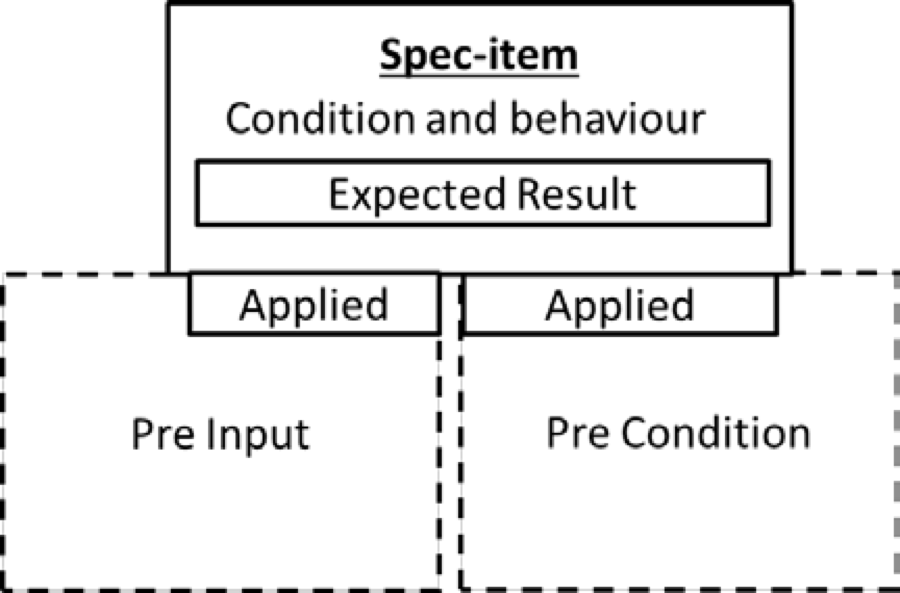
\includegraphics[width=10cm]{./image/D-4-Fig1.png}
  \caption{テスト条件の構成要素}
  \label{fig:D-4-Fig1}
  \end{center}
   \end{figure}

これらのテスト条件を合理的にある基準で網羅する方法を考える行為がテスト設計であり,そのための技法をテスト設計技法と呼ぶ.
テスト設計のアウトプットはテストケースである.

IEEE610では,テストケースを,特定の目的のために開発されたテスト入力,実行条件,期待結果の3つで構成されると定義している.
また,機能テストは,選択した入力と実行条件のレスポンスとして生成された出力を確認する,と定義している\cite{IEEE610}.
すなわち,機能テストとは,ブラックボックステストと同義である.
テスト入力,実行条件には,事前に設定されているものと,実行時点で設定するものがある.
おのおのは,表~\ref{tab:D-4-FigTPS}に示すよう分類できる.
% Table generated by Excel2LaTeX from sheet '論文挿絵'
\begin{table}[htbp]
  \centering
  \caption{テストの構成要素の再分類}
    \begin{tabular}{|l|l|l|}
    \hline
          & 事前に設定 (パラメータ)  & 実行時点で設定 (アクション)  \bigstrut\\
    \hline
    \hline
    テスト入力  & 事前入力  & イベント  \bigstrut\\
    \hline
    実行条件  & 事前状態  & 操作  \bigstrut\\
    \hline
    \end{tabular}%
  \label{tab:D-4-FigTPS}%
\end{table}%

その上で,本研究では,事前入力と事前条件をまとめたものをテストパラメータ,イベントと操作をまとめたものをテストアクションと呼ぶ\cite{yumoto2013-a}.
テスト条件を網羅するテストケースを開発する際,テストアクションは$Ta$から$Out$を導く直接的な要因である.
そのため,テストケースを実行する際の$Out$を導くテストアクションは1つに特定できる.
しかし,テストパラメータは,1つのテストアクションに対して多くのバリエーションを取り得る.
バリエーションは,事前入力となる$In$や$Ds$だけでなく事前状態となる$St$も含まれる.

\begin{figure}[h]
  \begin{center}
  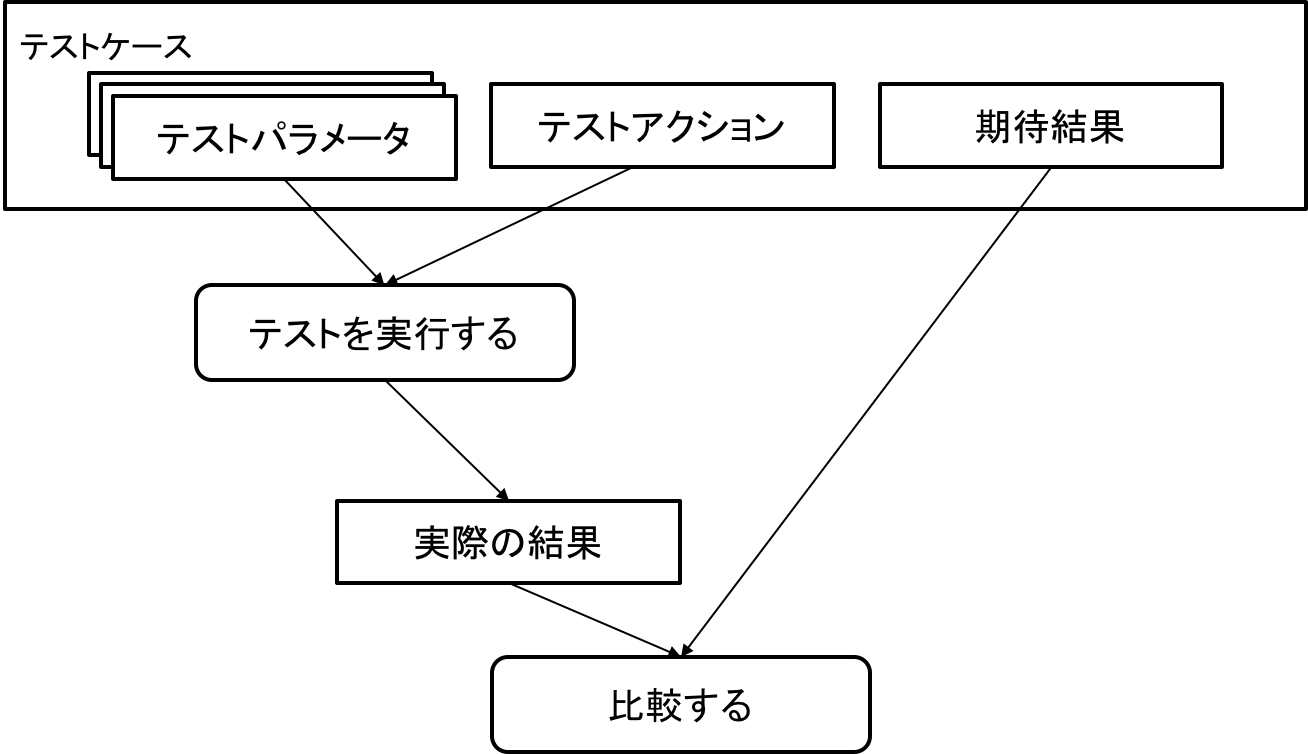
\includegraphics[width=10cm]{./image/D-2-FigTCS.png}
  \caption{テストケースを実行するプロセス}
  \label{fig:D-4-FigTCS}
  \end{center}
\end{figure}

ブラックボックステストのテストケースとテスト実行をするプロセスを図示すると,図~\ref{fig:D-4-FigTCS}のように表すことができる.
テスト入力,実行条件となるテストパラメータ,テストアクションを入力としてテストを実行し,出力した実際の結果が期待結果と一致するかを比較する.
期待と一致すればそのテストケースは成功であり,期待と一致しなければ,故障(Failure)として報告し,欠陥(Fault)が特定されれば,それを修正をすることになる.




\newpage
\section{テスト対象詳細化の問題} \label{sec:2-2}
\subsection{分類に対する一貫性の欠如}
テスト分析の活動のアウトプットとなるテスト条件は,機能,トランザクション,品質特性,構造的要素といったアプリケーションソフトウェアの側面の総称である\cite{ISTQB}.
これらの側面について記述した成果物は,仕様である.
ブラックボックステストのテスト分析では,テスト対象をテストケースが作れるサイズまで詳細化していく際に,これらの側面が記述してある仕様をベースにする.
詳細化する際は,テスト対象の詳細化をするときの起点や中間分類が人によって異なって違うものにならないよう分類の関係を定義して整理していく必要がある.
しかし,実務において,テスト分析におけるテスト条件群の整理方法は,経験則や個人の考え方に基づいている.

実務の世界では,一般的にテストベースを大項目,中項目,小項目と詳細化していくことが多い.
この方法は,詳細化する際の各分類項目にあてはめるアプリケーションソフトウェアの側面の分類方法に明確なルールが定義されていないため,個人毎の何かしらの考え方で詳細化するための分類を決めていくことになる.
そのため,複数人で作業を行うと分類にばらつきが発生し,同じ項目が複数の階層に現れてしまったり,同じ意味の項目が別の名称で選択されるといった混乱を引き起こす.
混乱が起きている例を表~\ref{tab:analysissample}に示す.
% Table generated by Excel2LaTeX from sheet '論文挿絵'
\begin{table}[htbp]
  \centering
  \caption{一般的なテスト分析の詳細化の例}
    \begin{tabular}{|l|l|l|l|p{5em}|p{6em}|}
    \hline
    大項目   & 中項目   & 小項目   & 細目    & 補足項目  & テスト条件 \bigstrut\\
    \hline
    \hline
    印刷    & 設定    & 印刷部数  & --    & --     & 100部印刷した場合 \bigstrut\\
    \hline
    設定    & プリント設定 & \shortstack{一般}  & 異常系 & \shortstack{エラー\\メッセージ} & 「印刷部数が99部を超えました」と表示されること \bigstrut\\
    \hline
    \end{tabular}%
  \label{tab:analysissample}%
\end{table}%

表~\ref{tab:analysissample}の例には,以下のような問題がある.
\begin{enumerate}
\item 設定というカテゴリが大項目に出ている場合と中項目に出ている場合が混在している.
\item 階層数も一定でないため,各階層がどのような意味を持つものかがばらついている.
\item 上段は,期待結果が書かれていない.
\item 上段と下段は同じテスト条件について書かれている.
\end{enumerate}
テスト開発の最初の活動であるテスト分析にて,詳細化で現れる項目の内容にこのような問題があると,その後の活動で作られるテストケースの抜け漏れ,重複に影響を及ぼす可能性が高くなると考えられる.
このような課題については,Eldhが,指示内容理解(Understanding Instruction)の不足によるテストケースの品質低下について調査をしており,複数の解釈による間違いが起きることを報告している\cite{eldh2011analysis}.

ISTQBでは,テスト分析の活動を「…テスト分析の期間中,何をテストするか決定するため,すなわち,テスト条件を決めるために,テストのベースとなるドキュメントを分析する」と説明している.
しかし,この説明は,テスト分析を実行するための要求事項や必要性は述べているだけであり,テストベースを分析していくための詳細化の方法を具体的に定義していない.
テスト分析手法に関する研究にて,詳細化するモデルがいくつか提案されている\cite{nishi2012based}
\cite{Akiyama2014}
\cite{morisaki2016}
\cite{mizuno2017test}
\cite{briand2002uml}.
しかし,複数の人数でテストケースを作る際に起きる課題については言及していない.テストケースを開発する人員の成熟度の向上は,重要な課題\cite{Basili:2006:EDS:1134285.1134291}\cite{itkonen2009testers}\cite{rooksby2009testing}であり,手法が有用であるための要因となる.

テストケースの開発に関する先行研究は,テスト分析にてテスト条件が特定された後のテスト設計で行われるテストパラメータの設計に焦点を当てている.
\cite{ammann1994using}
\cite{grochtmann1993classification}
\cite{demillo1978hints}
\cite{lehmann2000test}
テストパラメータを仕様書から自動摘出する研究
\cite{masuda2015semantic}
\cite{masuda2016detecting}
や,摘出したパラメータを使って仕様書とソースコードの比較をする研究
\cite{uetsuki2013efficient}
\cite{uetsuki2017improvement}
\cite{uetsuki2011software}
\cite{uetsuki2012decision}
などが進んでいる.
それらの研究では,テスト条件を特定するまでの詳細化はすでに行われた前提となっている.

\newpage
\section{機能間の統合に対するテストケース抽出の問題} \label{sec:2-3}
\subsection{既存の網羅基準によるテストケース数の増大}
テストケース数の増加は,単一機能のテストより機能間の統合において問題となる\cite{rehman2007testing}.
この場合のテストケース数は,単一の機能や制御構造の和で求めるのではなく,積となるためである.
それに加え,複数機能を統合したもののテストでは,状態遷移に伴う時系列の組み合わせのテストも求められることから,テストケース数の爆発問題が生じる.
テストケース数の爆発への対処としては,回帰テストにおけるテストケースの優先順位づけに関する研究がある\cite{rothermel2001prioritizing}
\cite{elbaum2000prioritizing}.
しかし,これらは,何かしらの基準に対する網羅性を示すものではない.
必要なテストケースの抽出方法とその網羅性に関する手法は,多くは機能や制御構造を基にした方法である.
そのため,機能間の統合と状態遷移に伴う時系列の組み合わせには対応していない.

状態遷移間の組み合わせに対するテストケースを開発するための手法は,数多く提案されている
\cite{whittaker1994markov}
\cite{lee1996principles}
\cite{fujiwara1991test}
\cite{andrews2005testing}.
状態遷移の組み合わせの網羅基準としては,Nスイッチカバレージがある.
Nスイッチカバレージでは,状態の遷移をパスとし,N+1 個の遷移パスを網羅する基準にしたがって組み合わせテストケースを抽出する\cite{chow1978testing}.
N=0 では遷移パスの組み合わせをテストできないため N=1,すなわち S1網羅基準(1スイッチカバレージ)が必要とされている.
しかし,S1網羅基準を満たすテストケース数は,2つの状態遷移間における遷移数の積となり,膨大なテスト工数が必要となる.

S1網羅基準の課題に対するアプローチとしては,自動化により工数を削減する研究とテストケース数を削減する先行研究がある.
自動化による工数削減の研究は,N-スイッチカバレージを満たすテストケースを形式仕様から自動生成する方法が知られている.
この方法は,テスト対象となるITシステムの動作を正確に記述したモデルを定義し,そのモデルから特定の長さの連続した遷移を抽出する方法である\cite{takagi2010concurrent}.
対象システムが運動方程式などに従う一般的なモデルベーステストと異なり,状態遷移にて生ずるシステムの動的な振舞いを形式仕様化する必要があり,それが困難であることから一般的なITシステムで適用された例は見当たらない.
生成されるテストケース数はN-スイッチカバレージと同じであり削減されないので,テストケースが自動抽出されても,実行のための操作は人手に頼る部分が残り,作業工数を合理化できない課題がある.

テストケース数を削減する研究としては,状態遷移の組み合わせに対して直交表を応用し2因子間の組み合わせを中心に,一部3因子の組み合わせも抽出する研究がある\cite{akiyama2007}\cite{akiyama2012}.
この方法は,デシジョンテーブルを用いて機械的に組み合わせを抽出でき,2因子間の組み合わせ即ちS0網羅基準は完全に網羅できるが,S1 網羅基準の網羅は不完全であり,かつその選択基準が用いた直交表に左右されるため重要なテストケースが漏れる課題がある.

現実的な方法としては,設計で用いられるUMLのシーケンス図を基にテストケースを抽出する方法が知られている\cite{hartmann2000uml}.
この方法によるテストケース数はシーケンス図で定義されたシーケンスで決まる.
シーケンス図が状態遷移のS1網羅基準を満たすか否かは,シーケンス図が表すテスト対象のサブセットの範囲による.
多くの場合,設計者が意図したシーケンスは,起こり得る状態遷移の組み合わせの一部しか表してないため,漏れが生じる課題がある.



\newpage
\section{テストカテゴリベースドテスト}
本研究では,テストカテゴリベースドテスト\cite{yumoto2013test}というテスト分析手法を利用した予備実験を行い,テスト分析の課題の調査,およびテスト分析の知識を与えることによるテストケースを網羅的に抽出できるスキル向上傾向の調査を行なった.
この結果は3章に記載をする.
この分析手法を使って調査を行う理由は,以下のとおりである.
\begin{enumerate}
\item 前述したテスト分析の問題のうち,分類に対する一貫性の欠如を解決するために自身で提案し,現場にて適用している手法である.
\item 実験のための題材となる仕様書,模範解答が揃っており,それらの題材を使って実験を行った研究結果がある.
\item 本研究で合理的にテストケースの抽出を行う手法を提案する基の考え方として,テストカテゴリベースドテストを利用していることである.
\end{enumerate}

本節では,テストカテゴリベースドテストの概要を説明する.
このテスト分析手法のアプローチでは,テスト対象のサブセットに属するタスクの仕様項目を特定していく方法を提示する.
また,テストケースの構造をベースにテスト条件を分解することで,テスト条件という用語の持つ曖昧さを排除する.
タスクとは,前述した通り,アプリケーションソフトウェアにて何らかの入力を出力に変換する処理のことである.
また,階層の要素としてテストカテゴリという,テスト対象の知識と故障の知識を使って定義した分類を構造に追加している.

\subsection{テスト条件群の構造}
前述した通り,テスト条件とは,機能,トランザクション,品質特性,構造的要素といったアプリケーションソフトウェアの側面の総称である.
通常,これらはアプリケーションソフトウェアの仕様として記載されるものである.
ブラックボックステストにおけるテスト条件群をテストケースの構成要素で整理すると,図~\ref{fig:D-2-FigTCStructure}に示した構造で整理できる.

\begin{figure}[htbp]
  \begin{center}
  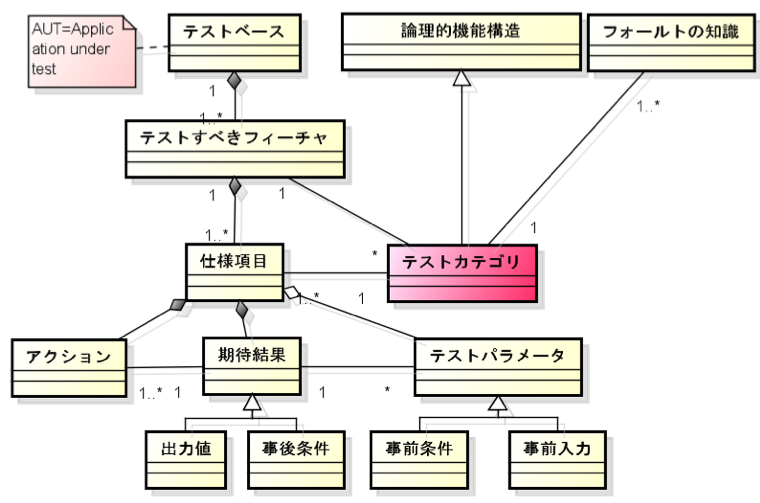
\includegraphics[width=10cm]{./image/D-2-FigTCStructure.png}
  \caption{テストケースの構成要素で整理したテスト条件の構造}
  \label{fig:D-2-FigTCStructure}
  \end{center}
   \end{figure}

テストベースは,テストケースを抽出する基になる文書のことであり,開発時に作成する要件や設計内容が書かれた文書が該当する.
テストベースにはフィーチャを実現するタスクを明確に定義する仕様項目が1つ以上記述されている.
フィーチャとは,利用者が観察可能なソフトウェアシステムの論理的なサブセットであり,利用者とテスト対象のインターフェースとなる\cite{kang1990feature}.
ブラックボックステストは,外部観察によるテスト設計の方法であるため,テスト条件をフィーチャから選択することが必要になる.
テスト対象となるフィーチャはISO/IEC/IEEE29119の定義に従い,フィーチャセットと呼ぶ\cite{ISO29119}.

仕様項目とは,フィーチャセットに属するタスクの要件を綿密に定義し文書化したものである.
タスクの要件とは,フィーチャセットの振る舞いの1つであり,たとえば「ボリュームは1から10の間で設定できる.1は消音であり,10は100dbsになる」が該当する.
この記述が仕様項目である.
テスト分析では,テストすべき仕様項目を特定していく.
その仕様項目の内容をテストケースの構成と同じように期待結果とテストパラメータに分類し,整理する.
テストパラメータとは,テストケースの構成要素の1つで,事前入力と事前条件を汎化したものである.
期待結果は,出力と事後条件を汎化したものである.
このような分類,整理によって,明確なルールにそったテスト分析が可能になる.

\subsection{論理的機能構造}
ブラックボックステストの場合,テスト対象の内部構造を完全に知ることはできなく,テスト実行は入力と出力だけが頼りになる.
大村は「…人工のシステムとは,インプットを変換し付加価値を与えアウトプットする変換装置であるため,論理的には,必ず図~\ref{fig:D-2-FigLSOF1}のような構造を持つ\cite{LSOF}」と主張している.
\begin{figure}[htbp]
  \begin{center}
	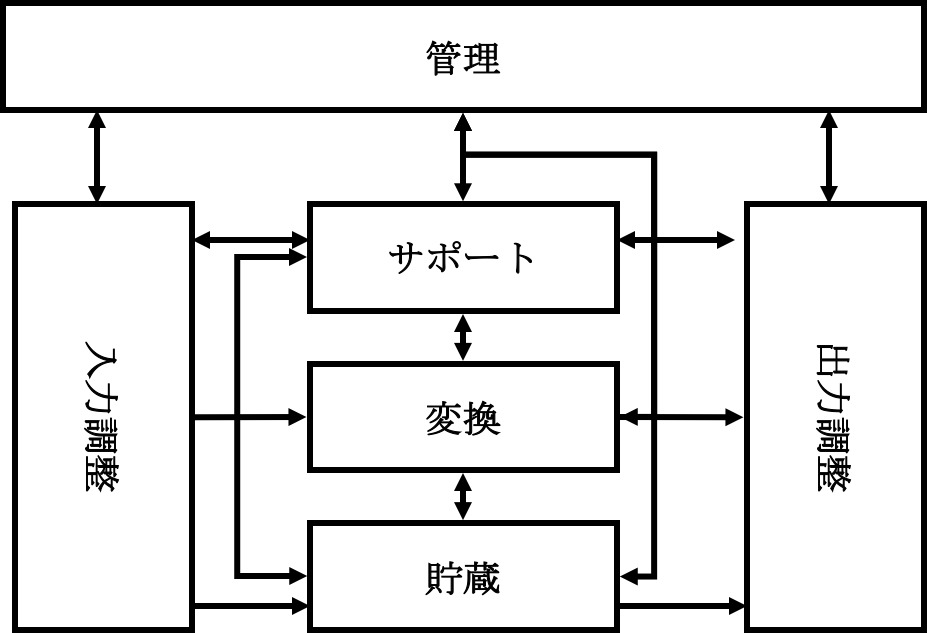
\includegraphics[width=10cm]{./image/D-2-FigLSOF.png}
	\caption{人工システムの論理構造}
	\label{fig:D-2-FigLSOF1}
  \end{center}
\end{figure}

\begin{description}
  \item[入力調整]入力される資源は,直接変換機能に送り込まれることなく,変換しやすいように入力機能によって整えられたのちに送り込まれる.
  \item[出力調整]不十分であったり不必要なものを含む変換されて出てくる資源をシステムから出力する前に,有用資源に調整したり不必要なものを始末する.
  \item[変換]システムの中核となる基本機能.システムが目的を達成するのに直接関わり,システムを特徴付ける.
  \item[貯蔵]入力資源を変換機能に安定的に供給したり,出力資源を外部の要求に合わせて送り出すために,さらには他の基本機能がスムーズに働くためにシステム内に資源を蓄える.
  \item[サポート]変換をはじめとする他の機能が円滑に働くために,それぞれの機能を裏から支える.
  \item[管理]変換装置全体が様々な制約の中で秩序関係を維持しながら目的を達成できるようにする.
\end{description}


テストカテゴリベースドテストは,同様のコンセプトを利用している.
つまり,テスト対象となるフィーチャセットは同様の論理構造を持つ人工システムだと捉える.
フィーチャをMECE(互いに相容れなくて完全に徹底的)\cite{ethan1999mckinsey}な方法でテストをするために,この論理構造を利用する.
テストカテゴリベースドテストでは,人工システムが持つ論理構造を基にして,図~\ref{fig:D-2-LSOF2}のように定義し,論理的機能構造と命名する.

\begin{figure}[htbp]
  \begin{center}
	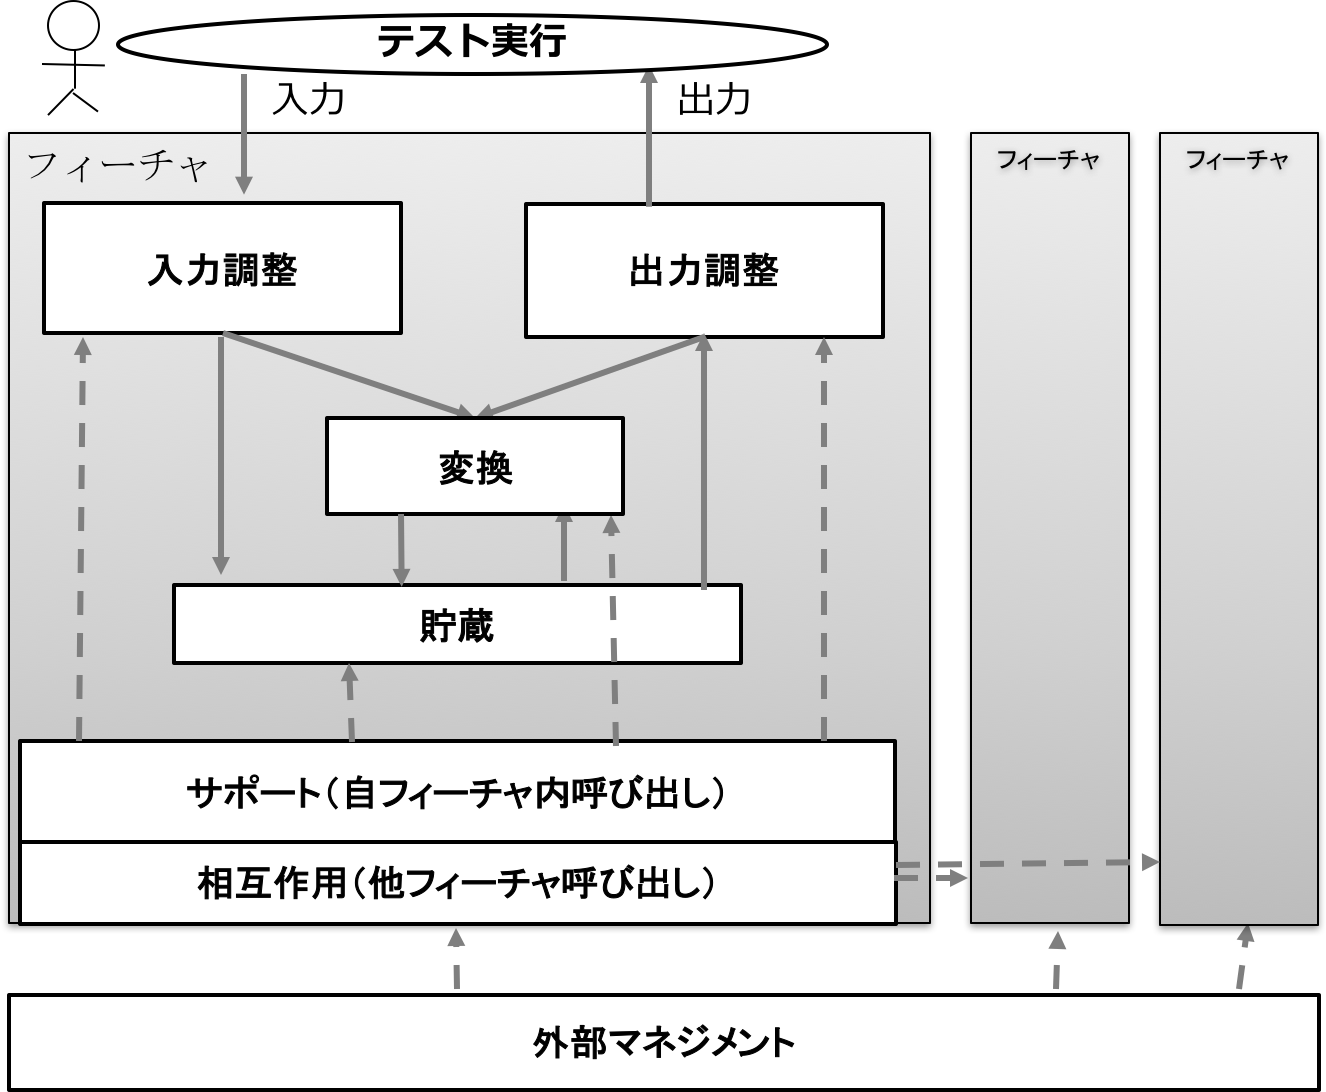
\includegraphics[width=10cm]{./image/D-3-Fig3.png}
	\caption{論理的機能構造}
	\label{fig:D-2-LSOF2}
  \end{center}
\end{figure}

図~\ref{fig:D-2-LSOF2}に示す各要素は,テスト対象の内部構造を推定し,テストが必要なタスクを特定する有用なモデルとして利用できる.論理的機能構造では,前述した人工システムの論理構造でサポートと呼んでいる要素をサポートと相互作用の二つに分けている.
サポートは,割り込みや同時処理のロック機構など,変換や貯蔵などフィーチャの内部に属するタスクが正しく処理を行うためのサポートタスクのテストのための分類である.通常,テスト対象のフィーチャに対する1回のテストアクションで確認できる.
相互作用は,変換や貯蔵などの内部に属するタスクでの処理の別タスクへの副作用の確認であり,通常,2回以上のテストアクションを必要とするものである.
管理は,外部マネジメントと呼び,フィーチャセットの外側で,システム全体の秩序を維持するタスクを分類する.
そのため,ブラックボックステストでは使わない.

飛行機のフライトを予約するシステムのシステムテストにて,「新規フライト予約」をフィーチャセットとした時のテスト条件を特定する例で考えてみる.
新規フライト予約では,まず予約したいフライトが何であるかをシステムに入力するが,過去の日付など購入できない日付や,運行していない行き先など,不正な入力情報をあらかじめチェックするタスクがあり,テストが必要となる.
これは入力調整へ分類する.
入力情報から,予約可能なフライトの購入金額を計算するタスクのテストは,変換に分類する.
そして,予約が成立するとその情報はシステムに登録される.登録を行うタスクのテストは貯蔵に分類する.
このシステムが状態を持っていて,状態によって予約ができないといった制御があれば,そのタスクに対するテストが必要になる.これはサポートに分類する.
また,予約が成立したことによる副作用を別のタスクに対するテストアクションで確認するテストは,相互作用に分類する.
外部へ結果を伝える際にフォーマットの変換を行うといったタスクがある.このタスクのテストは出力調整へ分類する.
このようなテストを実行するためには,タスクに関する振る舞いや条件が記述がされている仕様項目を特定する必要がある.この特定した仕様項目がテスト条件となる.


テスト分析をしていく際に,論理的機能構造を使って内部構造を推定してタスクを特定していく方法を導入すると,テストに必要なテスト条件の特定が容易になるという仮説を立てている.
現状,次に示す課題はテスト条件の特定を困難にしている.

\begin{enumerate}
\item 明白に必要だと思われる仕様の一部分が記述されていない.
\item 機能間の組み合わせでどのように振舞うかといった仕様は,テストベース中の該当する単一の節以外に記載される.
\end{enumerate}

\subsection{テストカテゴリ}
論理的機能構造は抽象的な概念であるため,テスト分析をするそれぞれの人員の間にて解釈の違いが生じる可能性がある.
テスト条件を決定する際に,その解釈に一貫性を持たせるため,論理的機能構造の要素に対してテスト対象で使われる用語を使った名前付けをする.
そのようなテスト対象に特化して付けた論理的機能構造の各要素の名前をテストカテゴリと呼ぶ.
テストカテゴリの命名には,テスト対象の知識が必要である.
そして,テストカテゴリは,テストケースの抽出に携わる各人員がテストカテゴリの意味を同じように理解することが必要であり,そのための合意形成を行う.
テスト対象を表す命名で合意したテストカテゴリは,テスト条件を特定するための有用なガイドとなる.

\begin{table}[htbp]
  \centering
  \caption{テストカテゴリ一覧の例}
    \begin{tabular}{|p{6em}|p{8.07em}|p{14.645em}|}
    \hline
    論理的構造 & テストカテゴリ & 意味づけ(想定する故障)\bigstrut\\
    \hline
    \hline
    \multirow{2}[4]{*}{入力調整} & 画面入力 & 入力チェック,入力画面の制御 \bigstrut\\
\cline{2-3}    \multicolumn{1}{|l|}{} & ボタン操作 & 画面遷移のルール,処理起動 \bigstrut\\
    \hline
      \multirow{2}[4]{*}{出力調整} & 表示& 処理結果の表示,出力数の制御 \bigstrut\\
\cline{2-3}
    \multicolumn{1}{|r|}{} & 帳票出力 & 印刷内容,印刷フォーマット \bigstrut\\
    \hline
    変換 & 計算 & 料金計算 \bigstrut\\
    \hline
    \multirow{2}[4]{*}{貯蔵} & 検索 & 検索条件の組み合わせ,検索結果 \bigstrut\\
\cline{2-3}    \multicolumn{1}{|l|}{} & 登録/更新/削除 & DB処理 \bigstrut\\
    \hline
    相互作用 & 反映 & DB処理結果の他機能への反映 \bigstrut\\
    \hline
    サポート & エラー処理 & エラー復旧処理\bigstrut\\
    \hline
    \end{tabular}%
  \label{tab:D-2-tabTCL}%
\end{table}

テストカテゴリは,表~\ref{tab:D-2-tabTCL}にて示したテストカテゴリ一覧にまとめる.
そして各テストカテゴリに分類したテストにて検出したいと考えている故障を列挙する.
これら故障に対して,テストケースを開発する人員の間で例を挙げてディスカッションし,
その結果を表~\ref{tab:D-2-tabTCL}で示したテストカテゴリ一覧の故障の欄に反映する.
ディスカッションにより,テスト開発プロセス活動にかかわる人員は,テストカテゴリの意味に対して合意形成をすることができる.
合意形成のねらいは次のとおりである.

\begin{enumerate}
\item テスト開発にかかわるテスト担当がフィーチャセットに対して同様の理解に達することができる.
\item テスト担当間のテスト条件の解釈のぶれを最小限にとどめることができる.
\end{enumerate}


\subsection{実施手順}
構造化したテスト条件群を順番に導くために,テスト分析の活動を図~\ref{fig:D-2-FigStep}のような作業ステップに分割し,各ステップでのインプットとアウトプットを定義する.


\begin{figure}[htbp]
  \begin{center}
  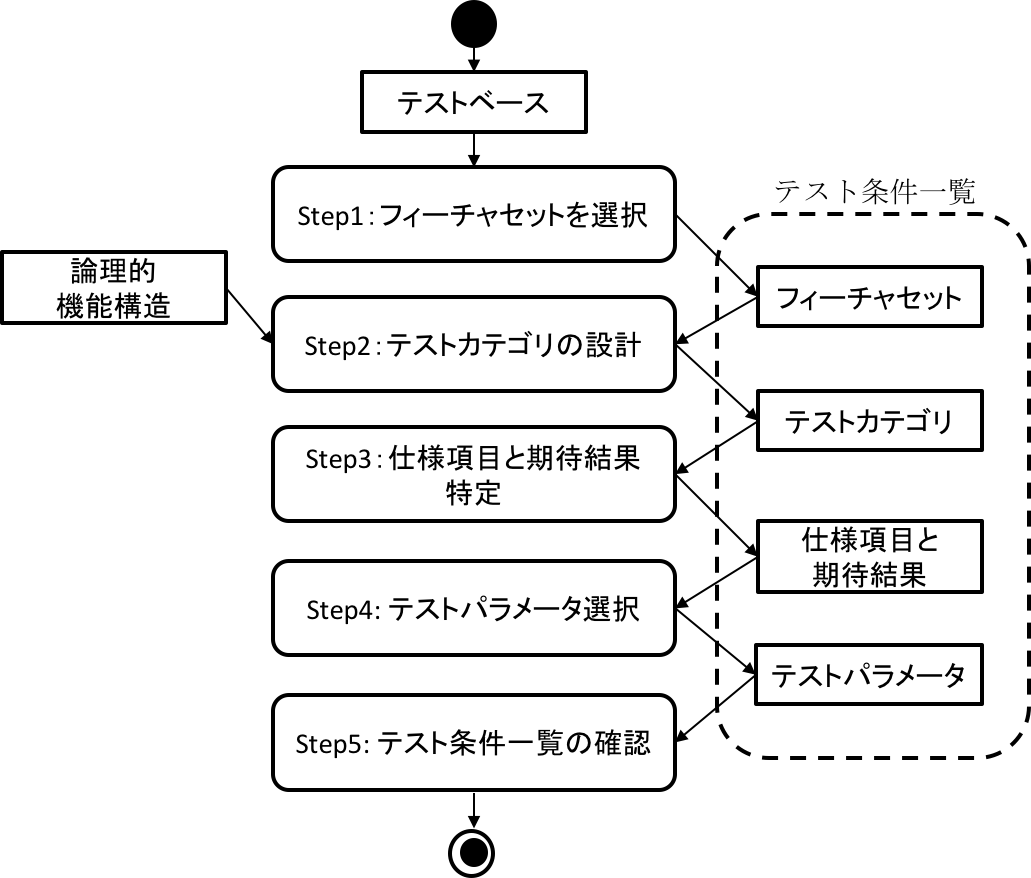
\includegraphics[width=12cm]{./image/D-2-FigStep.png}
  \caption{テスト分析の実行ステップ}
  \label{fig:D-2-FigStep}
  \end{center}
   \end{figure}


以降に各作業ステップについて説明をする.

\begin{description}
\item[Step1] フィーチャセットを選択

テストベースからテスト対象のサブセットとなるフィーチャセットを特定する.
フライト予約をするアプリケーションソフトウェアで例えた場合,新規フライト予約(搭乗したい飛行機の条件を照合し,予約を成立させる一連の機能群)がフィーチャセットとなる.

\item[Step2] テストカテゴリの設計

テストカテゴリを設計する方法は,階層ホログラフィックモデリング法(HHM法)におけるサブトピックの設定方法と類似している\cite{HHM2002}.
HHM法でいうところのメイントピックにフィーチャセットを置く.
メイントピックを構成するサブトピックとして論理的構造毎にフィーチャセットの動作条件や振る舞いを列挙する.
列挙する際は,どのような故障が起きることが考えられるかを検討材料にして列挙する.
選択したフィーチャセット全部に対してサブトピックを列挙した後に,サブトピック全体を眺めて,象徴する名称を付与し,それをテストカテゴリにする.
テストカテゴリは,メンバ間で内容を説明し,意味づけ(どのような故障が起きるか)を共有することで,解釈のぶれを防ぐ.


\item[Step3] テストカテゴリを使い仕様項目と期待結果を特定,整理する.

テストカテゴリでフィーチャの内部構造を推定し,実現するタスクを特定する.
テストベースからそのタスクの仕様項目と期待結果の記述を抽出する.


\item[Step4] テストパラメータを選択し,整理する.

特定した仕様項目と期待結果からテストパラメータを選択する.テストパラメータは特定した仕様項目と期待結果にそってテストベースを分析して選択する.

\end{description}



% Table generated by Excel2LaTeX from sheet 'Sheet2'
\begin{table}[htbp]
  \centering
  \caption{テスト条件一覧の例}
    \begin{tabular}{|c|p{6.8em}|p{4em}|p{4em}|p{7.6em}|}
    \hline
    \multicolumn{1}{|p{7.6em}|}{フィーチャセット} & テストカテゴリ & 仕様項目 & 期待結果 & テストパラメータ \bigstrut \\
    \hline
    \hline
    \multicolumn{1}{|c|}{\multirow{4}[8]{*}{TF-a}} & TC-a  & SI-a  & ER-a  & TP1,TP2 \bigstrut\\
\cline{2-5}          & \multicolumn{1}{l|}{} & SI-b  & ER-b-1 & TP1,TP3,TP4 \bigstrut\\
\cline{2-5}          & \multicolumn{1}{l|}{} & \multicolumn{1}{l|}{} & ER-b-2 & TP1,TP4 \bigstrut\\
\cline{2-5}          & TC-b  & SI-c  & ER-c  & TP5,TP6,TP7 \bigstrut\\
    \hline
    \multicolumn{1}{|c|}{\multirow{2}[4]{*}{TF-b}} & TC-a  & SI-d  & ER-d  & TP9,TP10 \bigstrut\\
\cline{2-5}          & TC-b  & N/A   & N/A   & N/A \bigstrut\\
    \hline
    \end{tabular}%
  \label{tab:D-2testconditionliset}%
\end{table}%

テストベースからテスト条件を特定する際は,その結果を表~\ref{tab:D-2testconditionliset}に示すテスト条件一覧にまとめる.

テスト条件一覧の最初の列には,フィーチャセットを列挙する.
各フィーチャセットの隣には,テストカテゴリのセットを列挙する.
そして,各テストカテゴリに対応する仕様項目と期待結果を列挙する.
フィーチャセットによってはテストカテゴリに対応する仕様項目が無い場合もある.
その場合はテストカテゴリの中に列挙されるものが何も無いため,N/Aと記載する.


仕様項目によっては,期待結果が複数になることがある.
その際は,1つの仕様項目に対して複数の期待結果を記載する.
テストパラメータには,各仕様項目と期待結果のセットから見て適切なテストパラメータの組み合わせを選択する.
テストパラメータは,テスト分析の後の活動となるテスト設計にて同値分割を行い適切な同値クラスにする.
複数の同値分割の組み合わせは,ディシジョンテーブル技法やペアワイズテスト技法といったテスト設計技法使って適切な組み合わせを設計する.

テストケースの開発に従事する多くの人員が上記のステップに従うと,同じルールにしたがって分析を行うことができる.
結果として,特定したテスト条件の一覧は,包括的で,重複が含まれない.
このようなテスト条件一覧を作成することは,高いテストカバレッジを確かにし,高品質なテストを提供することにつながる.
これは本手法の主たる効果となる.
更に,この手順にしたがってテスト分析を行うことには,以下の3つの効果がある.

\begin{enumerate}
\item この手順は,図~\ref{fig:D-2-FigTCStructure}で示した「テストケースの構成要素で整理したテスト条件の構造」
をベースにしている.この手順を通して,テストベースを仕様項目,期待結果,テストパラメータをそれぞれ順番に特定,選択していく.
テストケースの開発に携わる人員は,テスト分析の活動を通じて同じ順番でテスト条件を特定し同じカテゴリに分類できるため,全員の成果物をまとめて確認する際の可読性が向上する.
\item テストカテゴリに対する合意形成によって,テストケースの開発に携わる人員は仕様項目の特定と選択を同じ認識を持って行うことができる.人員間での情報共有も容易になる.
\item 本手法は体系化,標準化して進めていくことが容易になるため,組織に関わるテストケースの開発に携わる人員がテスト分析を繰り返すことができるようになる.
\end{enumerate}

\subsection{テスト条件特定結果の比較}

テストケースの開発に関するワークショップを開催し,同一組織内にてソフトウェアテストに従事している人員を2グループに分けて,テストカテゴリベースドテストの説明で記したテスト分析の作業「Step3:テストカテゴリを使った仕様項目と期待結果の選択」の演習を行った.

1つのグループは,テストカテゴリを使わずに仕様項目,期待結果,テストパラメータを列挙し,もう1つのグループは,テストカテゴリを使って仕様項目,期待結果,テストパラメータを列挙した.
題材として音楽再生機器を選定した.出席者はすべて類似の機器のシステムテストに関わった経験があり,製品知識はある.
フィーチャセットは,音楽再生機器のボリュームコントロールである.

2つの演習結果と演習の模範解答を比較し,解答例と同じだけの仕様項目を特定できれば網羅的に分析ができているとした.
そして,テストカテゴリベースドテストを適用した場合とそうでない場合の違いを分析した.
グループの回答を比較データに使った理由は,この手法の効果が複数の人員でテスト分析をしたときのばらつきからくる欠損や重複を防ぐことを狙っているためである.

% Table generated by Excel2LaTeX from sheet '集計 (J)'
\begin{table}[htbp]
  \centering
  \caption{仕様項目の選択割合の比較}
    \begin{tabular}{|l|r|r|r|r|r|r|r|r|r|r|r|r|}
    \hline
          & \multicolumn{1}{p{2em}|}{入力調整} & \multicolumn{2}{c|}{変換} & \multicolumn{2}{p{4em}|}{サポート} & \multicolumn{2}{p{2em}|}{出力調整} & \multicolumn{2}{c|}{貯蔵} & \multicolumn{1}{p{2em}|}{相互作用} & \multicolumn{1}{l|}{合計} & \multicolumn{1}{l|}{比率} \bigstrut\\
    \hline
    \hline
    解答例   & 0     & 2     & 1     & 0     & 2     & 1     & 0     & 1     & 0     & 2     & 9     & 100\% \bigstrut\\
    \cline{1-13}
    \multicolumn{1}{|p{7em}|}{テストカテゴリ未適用}  & 0     & 2     & 0     & 0     & 0     & 1     & 0     & 1     & 0     & 1     & 5     & 56\% \bigstrut\\
    \cline{1-13}
    \multicolumn{1}{|p{7em}|}{テストカテゴリ適用}  & 0     & 2     & 0     & 0     & 2     & 1     & 0     & 1     & 0     & 1     & 7     & 78\% \bigstrut\\
    \hline
    \end{tabular}%
  \label{tab:D-2-SICompare}%
\end{table}%

演習結果にて,仕様項目の選択数を比較すると表~\ref{tab:D-2-SICompare}のようになった.
1番上の行は解答例であり,講師が予め準備したものである.
2番目と3番目の行はワークショップの中で各グループが演習中に作成したものである.
比率は,解答例を母数にした場合の合計数の割合である.
テストカテゴリを利用したグループは講師と同じテストカテゴリを利用し,テストカテゴリを利用していないグループは,演習後にこちらでテストカテゴリにマッピングして比較可能にした.
両方のグループとも解答例と同じ数の仕様項目の特定はできなかった.
グループ間の比較をした場合,テストカテゴリありのグループのほうが仕様項目の特定数が2つ多く,より高い結果となった.

また,各仕様項目として列挙した期待結果とテストパラメータ数の集計は表~\ref{tab:D-2-resilt2}のような結果となった.

% Table generated by Excel2LaTeX from sheet '集計 (J)'
\begin{table}[htbp]
  \centering
  \caption{期待結果とテストパラメータ数の選択結果}
    \begin{tabular}{|l|r|r|r|r|r|r|}
    \hline
    \multirow{2}[4]{*}{テストカテゴリ} & \multicolumn{2}{c|}{仕様項目} & \multicolumn{2}{c|}{期待結果数} & \multicolumn{2}{c|}{パラメータ数} \bigstrut\\
\cline{2-7}          & \multicolumn{1}{l|}{適用なし} & \multicolumn{1}{l|}{適用あり} & \multicolumn{1}{l|}{適用なし} & \multicolumn{1}{l|}{適用あり} & \multicolumn{1}{l|}{適用なし} & \multicolumn{1}{l|}{適用あり} \bigstrut\\
    \hline
    \hline
    入力A   &       &       & \multicolumn{1}{l|}{N/A} & \multicolumn{1}{l|}{N/A} & \multicolumn{1}{l|}{N/A} & \multicolumn{1}{l|}{N/A} \bigstrut\\
    \hline
    \multirow{2}[4]{*}{変換A} & \multicolumn{1}{c|}{○} & \multicolumn{1}{c|}{○} & 1     & 1     & 5(3)  & \multicolumn{1}{l|}{N/A} \bigstrut\\
\cline{2-7}          & \multicolumn{1}{c|}{○} & \multicolumn{1}{c|}{○} & \multicolumn{1}{l|}{N/A} & 1     & 1     & \multicolumn{1}{l|}{N/A} \bigstrut\\
    \hline
    変換B   &       &       & \multicolumn{1}{l|}{N/A} & \multicolumn{1}{l|}{N/A} & \multicolumn{1}{l|}{N/A} & \multicolumn{1}{l|}{N/A} \bigstrut\\
    \hline
    サポートA &       &       & \multicolumn{1}{l|}{N/A} & \multicolumn{1}{l|}{N/A} & \multicolumn{1}{l|}{N/A} & \multicolumn{1}{l|}{N/A} \bigstrut\\
    \hline
    \multirow{2}[4]{*}{サポートB} &       & \multicolumn{1}{c|}{○} & \multicolumn{1}{l|}{N/A} & 1     & \multicolumn{1}{l|}{N/A} & 2 \bigstrut\\
\cline{2-7}          &       & \multicolumn{1}{c|}{○} & \multicolumn{1}{l|}{N/A} & 1     & \multicolumn{1}{l|}{N/A} & 2 \bigstrut\\
    \hline
    出力A   & \multicolumn{1}{c|}{○} & \multicolumn{1}{c|}{○} & 1     & 1     & \multicolumn{1}{l|}{N/A} & 2 \bigstrut\\
    \hline
    出力B   &       &       & \multicolumn{1}{l|}{N/A} & \multicolumn{1}{l|}{N/A} & \multicolumn{1}{l|}{N/A} & \multicolumn{1}{l|}{N/A} \bigstrut\\
    \hline
    貯蔵A   & \multicolumn{1}{c|}{○} & \multicolumn{1}{c|}{○} & 1     & 1     & 3(1)  & 2 \bigstrut\\
    \hline
    貯蔵B   &       &       & \multicolumn{1}{l|}{N/A} & \multicolumn{1}{l|}{N/A} & \multicolumn{1}{l|}{N/A} & \multicolumn{1}{l|}{N/A} \bigstrut\\
    \hline
    \multirow{2}[4]{*}{相互作用A} & \multicolumn{1}{c|}{○} & \multicolumn{1}{c|}{○} & \multicolumn{1}{l|}{N/A} & 1     & 1     & 1 \bigstrut\\
\cline{2-7}          &       &       & \multicolumn{1}{l|}{N/A} & \multicolumn{1}{l|}{N/A} & \multicolumn{1}{l|}{N/A} & \multicolumn{1}{l|}{N/A} \bigstrut\\
    \hline
    合計    & 5     & 7     & 3     & 7     & 10(4) & 9(0) \bigstrut\\
    \hline
    \end{tabular}%
  \label{tab:D-2-resilt2}%
\end{table}%


テストカテゴリを利用しなかったグループは,期待結果が明記されていなく,テストパラメータをあらわすテスト条件のみ記載している仕様項目がテストカテゴリを利用したグループと比較して4つ多かった.
列挙されていたパラメータ数は,テストカテゴリを利用しないグループのほうが11多く,4倍以上であった.
また,テストパラメータの内容を被験者に確認して,同じ仕様項目のパラメータになるものが別の仕様項目として記述されていたものを講師が集計時に分類し直した.パラメータ数の欄に()にて記した.
テストカテゴリを利用しないグループは,パラメータ数の欄に()で記した数が4つあった.
これらはテスト設計時に重複したテストケースを設計してしまう可能性がある.

\section{まとめ}
本章では,研究の対象となるアプリケーションソフトウェア,テストケースの種類,テストレベル,テストプロセスを明記し,ソフトウェアテストの中で,システムテストレベルでのブラックボックステストを研究の対象にすること,ブラックボックステストのテストケースを開発する活動の中では,テスト分析を対象にすることを述べた.
そして,そこで起きている問題として,テスト対象を詳細化するときに分類に対する一貫性が欠如していることを述べた.また,機能間の統合に対する問題として,既存の網羅ベース準を適用するとテストケース数が膨大になることを述べた.

これらの問題に対して,テストカテゴリベースドテストというテスト分析手法をベースに研究をすすめるため,前提知識としてこの手法の概要と,既出の実験結果を説明した.

%%%%%%%%%%%%%%%%%%%%%%%
\chapter{テスト分析でのばらつき傾向とテストケース抜け漏れへの影響}\label{chap:3}
本章では,前章で述べた課題を更に分析するためにおこなった予備実験の結果を述べる.
実験では,被験者に対して,テストベースを与えてテスト分析を実施してもらい,その後,テスト分析手法であるテストカテゴリベースドテストの知識を与えた上で再度テスト分析をしてもらう.
テスト分析手法の知識を与える前と後の結果から,ルールがない状態でのテスト分析結果にはばらつきがあること,また,2章で説明をしたテストカテゴリベースドテストによるルールを与えることによる変化を調査する.

\newpage
\section{予備実験の目的} \label{sec:3-1}
2.4節の「テストカテゴリベースドテスト」にて示した実験では,分析手法を適用したグループが,導入していないグループよりも抜け漏れが少なく重複も少ない結果となった.
しかし,実験データは1組のみであり,傾向を結論づけるには不十分である.
テスト分析手法を適用する前のテスト分析での結果のばらつきの傾向,及びばらつきの傾向と分析手法を適用後の結果との相関をより多くのデータで調べることを目的にした予備実験を行った.
実験はワークショップを通じてグループ単位で2回,個人単位で1回行なった.
\begin{description}
  \item[グループ単位1] 製造メーカーの同一製品開発チームのメンバーを4〜5人にグルーピングして実施(6サンプル収集)
  \item[グループ単位2] オープンな研修にて,別々の企業の参加者を4〜5人にグルーピングして実施(2サンプル収集)
  \item[個人単位1] テスト技術者コミュニティ主催のワークショップを通じて実施(57サンプルを収集)
\end{description}

\newpage
\section{グループ単位の実験}
\subsection{実験の概要}
グループ単位の実験は2回行った.
両方とも4時間のワークショップを通じて実施した.
ワークショップの進め方を,図~\ref{fig:D-3-ExparimentAbst1}に示す.最初に,テスト開発プロセスを説明する.その後,演習に使うテストベースを示し,参加者に各自の考えに基づき,2.4.5節の実験と同様に「テスト分析の作業Step3:テストカテゴリを使った仕様項目と期待結果の選択」を実施してもらう.
その後,4〜5名の参加者をランダムにグルーピングし,グループ内で各自のテスト分析の結果をグループの回答としてまとめる.

最初の分析結果のまとめが終わり,全出席者のが各グループの分析結果を理解した後,テストカテゴリを用いたテスト分析手法と実施手順を説明して,手法の手順に沿って再度テスト分析を参加者が各自で実施する.
その後は最初の分析結果同様にグループの回答をまとめる.

解答例と同じだけの仕様項目を特定できれば網羅的にテスト分析ができているとする.
そのうえで,同一グループに対するテスト分析手法の知識を与える前と,知識を与えた後のグループ回答を実験のデータとして利用した.
\begin{figure}[h]
\begin{center}
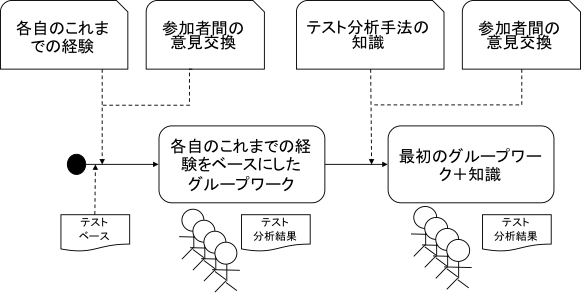
\includegraphics[width=10cm]{./image/D-3-ExparimentAbst1.png}
\caption{演習の前提条件の変化}
\label{fig:D-3-ExparimentAbst1}
\end{center}
\end{figure}

\subsection{実験の題材}
実験の題材は2種類用意した.
[グループ単位1]では,組込みソフトウェア開発の演習題材として音楽再生機器を使った.フィーチャーセットはボリュームコントロール機能を対象にした.2.4.5節で行なった実験とは別の製品の仕様書を題材にしている.
[グループ単位2]では,エンタープライズシステム開発の演習題材として,フライト予約Webシステムを利用した.フィーチャーセットは新規フライト予約である.
テストベースとなる仕様書として,両方とも12枚のパワーポイントのスライドを用意した.
講師側が用意した解答例である,テスト分析で特定すべきテスト条件の一覧を表~\ref{tab:D-3-ensyu1}と表~\ref{tab:D-3-ensyu2}に示す.

% Table generated by Excel2LaTeX from sheet 'Sheet1'
\begin{table}[htbp]
 \footnotesize
  \centering
  \caption{音楽再生機器の講師解答例}
% Table generated by Excel2LaTeX from sheet 'Sheet1'
    \begin{tabular}{|c|l|p{11em}|p{11em}|}
    \hline
    \multicolumn{1}{|p{7em}|}{{論理的機能構造}} & \multicolumn{1}{p{8em}|}{{テストカテゴリ}} & {仕様項目} & {期待結果/確認内容} \bigstrut\\
    \hline
    \hline
    \multicolumn{1}{|c|}{\multirow{2}[4]{*}{{入力調整}}} & \multicolumn{1}{p{7.75em}|}{{対向機入力}} & {--} & {--} \bigstrut\\
\cline{2-4}          & \multicolumn{1}{p{7.75em}|}{{ボタン}} & {・キューイング} & {・早押ししたとき無視すること} \bigstrut\\
    \hline
    \multicolumn{1}{|c|}{\multirow{2}[4]{*}{{出力調整}}} & \multicolumn{1}{p{7.75em}|}{{音声出力}} & {・ボリューム上限下限を知らせるビープ音} & {・ビープ音が押下に対して1回なること} \bigstrut\\
\cline{2-4}          & \multicolumn{1}{p{7.75em}|}{{LED点灯}} & {--} & {--} \bigstrut\\
    \hline
    \multicolumn{1}{|c|}{\multirow{2}[4]{*}{{変換}}} & \multicolumn{1}{p{7.75em}|}{{音量}} & {・音量調節} & {・ボタン押下でボリュームが上下すること} \bigstrut\\
\cline{2-4}          & \multicolumn{1}{p{7.75em}|}{{対向機操作}} & {-} & \multicolumn{1}{r|}{} \bigstrut\\
    \hline
    \multicolumn{1}{|c|}{\multirow{2}[2]{*}{{貯蔵}}} & \multicolumn{1}{l|}{\multirow{2}[2]{*}{{設定保存}}} & {・デフォルト値} & {・ボリュームを変更させてリセットするとデフォルト値に戻ることで確認} \bigstrut[t]\\
          &       & {・音量調節の保存} & {・PowerON後前回Offした際の結果と同じ音量がでることを確認する} \bigstrut[b]\\
    \hline
    \multicolumn{1}{|p{5.835em}|}{{サポート}} & \multicolumn{1}{p{7.75em}|}{{ヘッドセット状態遷移}} & {・状態により音量調節アクションを受け付ける/受け付けない} & {・再生中、通話中以外音量調節ボタンを無視する} \bigstrut\\
    \hline
    \multicolumn{1}{|c|}{\multirow{3}[4]{*}{{相互作用}}} & \multicolumn{1}{p{7.75em}|}{{対向機への反映}} & {・対向機のボリューム値への影響} & {・ヘッドセットのボリュームを変更したあと、対向機のボリュームが変更していないことで確認} \bigstrut\\
\cline{2-4}          & \multicolumn{1}{l|}{\multirow{2}[2]{*}{{設定情報の共有}}} & {・複数の設定情報の設定影響} & {・通話と再生で交互に音量を調節した際に互いに影響を受けないこと} \bigstrut[t]\\
          &       & {・他の処理で音量設定の削除} & {・初期化、リセットで初期値に戻ることを確認} \bigstrut[b]\\
    \hline
    \end{tabular}%
  \label{tab:D-3-ensyu1}%
\end{table}%



% Table generated by Excel2LaTeX from sheet 'Sheet1'
\begin{table}[htbp]
\footnotesize
  \centering
  \caption{フライト予約システムの講師解答例}
    \begin{tabular}{|c|l|p{10.5em}|p{13em}|}
    \hline
    \multicolumn{1}{|p{7em}|}{論理的機能構造} & \multicolumn{1}{p{7em}|}{テストカテゴリ} & 仕様項目  & 期待結果/確認内容 \bigstrut\\
    \hline
    \hline
    \multicolumn{1}{|c|}{\multirow{9}[4]{*}{入力調整}} & \multicolumn{1}{l|}{\multirow{8}[2]{*}{画面入力}} & ・画面表示内容 & ・画面仕様書に沿ったレイアウトであること \bigstrut[t]\\
          &       & ・年、月、日の入力範囲チェック & ・入力フィールド/ボタンの制御が仕様どおりであること \\
          &       & ・入力桁数チェック & ・Min日以降Max日が入力できること\\
          &       & ・型チェック & ・フライト予約可能日以前の入力はクリアされること\\
          &       & ・うるう年判定、末日判定 & ・桁数/文字数チェックをすること\\
          &       & ・出発地と到着地の組合せ & ・型(文字,数値)のチェックをすること\\
          &       & \multicolumn{1}{r|}{} & ・うるう年、末日判定のチェックをすること \\
          &       & \multicolumn{1}{r|}{} & ・同じ出発地と到着地を選択できないこと \bigstrut[b]\\
\cline{2-4}          & \multicolumn{1}{p{7.75em}|}{ボタン操作} & ・画面遷移 & ・画面仕様書に沿った画面の遷移ができること \bigstrut\\
    \hline
    \multicolumn{1}{|c|}{\multirow{6}[4]{*}{出力調整}} & \multicolumn{1}{l|}{\multirow{5}[2]{*}{結果表示}} & ・プログレスバー/登録完了メッセージ & ・登録中と登録後表示が正しいこと \bigstrut[t]\\
          &       & ・注文不成立メッセージ & ・メッセージが出ること \\
          &       & ・金額計算表示 & ・フィールドに収まること \\
          &       & ・注文番号 & ・同上 \\
          &       & ・フライト情報 & ・同上\bigstrut[b]\\
\cline{2-4}          & \multicolumn{1}{p{7.75em}|}{帳票出力} & --    & -- \bigstrut\\
    \hline
    \multicolumn{1}{|c|}{\multirow{3}[2]{*}{変換}} & \multicolumn{1}{l|}{\multirow{4}[2]{*}{計算}} & ・合計額の計算 & ・クラス単価×人数となること \bigstrut[t]\\
          &       & ・登録時の採番 & ・直前のNo+1となること \\
          &       & ・チケット在庫の計算 & ・在庫数から購入数をマイナスし0以下にできない \\
    \hline
    \multicolumn{1}{|c|}{\multirow{2}[4]{*}{貯蔵}} & \multicolumn{1}{p{7.75em}|}{検索} & ・フライト検索結果 & ・検索条件(and)で該当するフライトが検索されること \bigstrut\\
\cline{2-4}          & \multicolumn{1}{p{7.75em}|}{登録、更新、削除} & ・フライトの登録 & ・フライトが登録が出来ること \bigstrut\\
    \hline
    \multicolumn{1}{|c|}{\multirow{2}[2]{*}{サポート}} & \multicolumn{1}{l|}{\multirow{2}[2]{*}{エラー処理}} & ・登録時にチケット在庫なし & ・エラーになること\bigstrut[t]\\
          &       & ・注文挿入中の強制終了 & ・ロールバックすること \bigstrut[b]\\
    \hline
    \multicolumn{1}{|c|}{\multirow{3}[2]{*}{相互作用}} & \multicolumn{1}{l|}{\multirow{3}[2]{*}{反映}} & ・「既存注文開く」への反映 & ・検索条件(and)で検索されること \bigstrut[t]\\
          &       & ・「注文件数グラフ」への反映 & ・注文件数がプラスされること \\
          &       & ・「注文履歴」への反映 & ・全ての状況(登録)が書き込まれること \bigstrut[b]\\
    \hline
    \end{tabular}%
  \label{tab:D-3-ensyu2}%
\end{table}%

\subsection{テスト分析手法適用前のテスト分析の結果}

ルールがない状態でのテスト分析結果のばらつきについて,実験による典型的な4パターンのテスト分析結果を図 ~\ref{fig:D-3-Fig1-1}から図 ~\ref{fig:D-3-Fig1-4}で示す.
\begin{enumerate}
\item CS1 と CS2:両方ともテスト対象の入力フィールドを行タイトルに列挙している.しかしながら列名と表の内容が異なっている.
\item CS3: 表の中に記載されている各列,アクションとパラメータと期待結果などが独立しているため,それぞれの間の関連を特定できない.
\item CS4: テスト対象の状態が列名として列挙されている.各状態で取りうるパラメータと値が表の中に記載されている.
\end{enumerate}

この結果は複数の個人のテスト分析が,それぞれ複数の結果に到達することを示している.
複数の結果とは,テスト分析を通して特定したテスト条件にばらつきがあることを意味している.
テスト分析が多くの人たちで行われるときには,テスト条件の重複,もしくは完全に抜け落ちるといった可能性が非常に高くなると考えられる.
仮説として,テストカテゴリベースドテストの知識を与えることで,ルールが適用されるため,テスト条件の特定できる数が増加すると考えられる.

\begin{figure}[H]
\centering
\subfloat[テスト分析の事例:CS1]{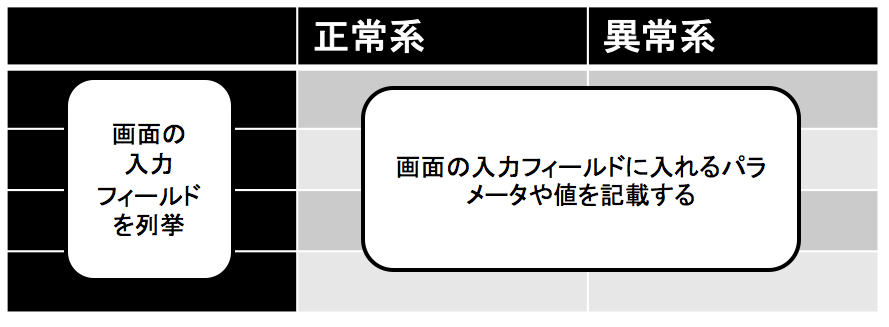
\includegraphics[clip, width=4in]{./image/D-3-Fig1-1.png}
\label{fig:D-3-Fig1-1}}
\\
\subfloat[テスト分析の事例:CS2]{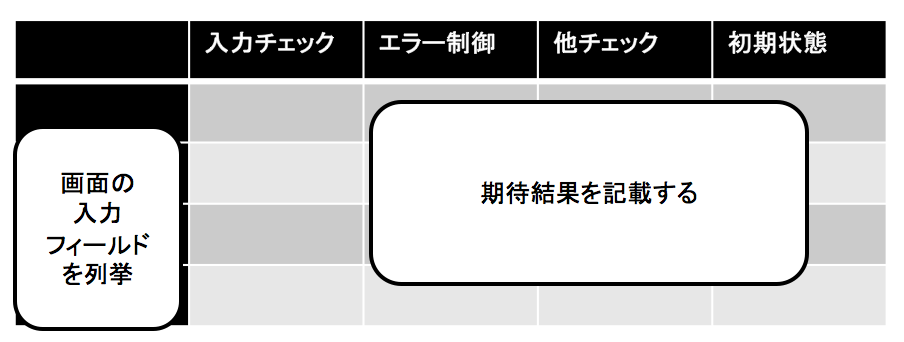
\includegraphics[clip, width=4in]{./image/D-3-Fig1-2.png}
\label{fig:D-3-Fig1-2}}
\\
\subfloat[テスト分析の事例:CS3]{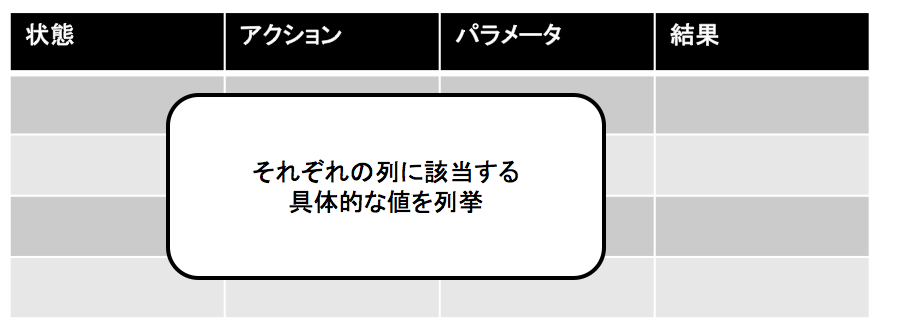
\includegraphics[clip, width=4in]{./image/D-3-Fig1-3.png}
\label{fig:D-3-Fig1-3}}
\\
\subfloat[テスト分析の事例:CS4]{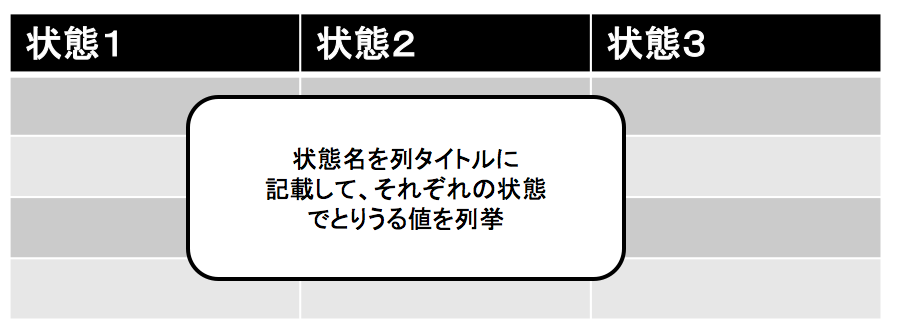
\includegraphics[clip, width=4in]{./image/D-3-Fig1-4.png}
\label{fig:D-3-Fig1-4}}
\caption{テスト分析の事例}
\label{fig:D-3-Fig1-1234}
\end{figure}


\subsection{実験結果の評価}
1回目,2回目の実験では,グループでの回答を実験結果として利用した.
1回目の実験は,組み込み開発を行なっている組織内での6チームの実験結果を収集し
2回目の実験結果ではオープンセミナーの参加者をグルーピングした2つの実験結果を収集したので,合計で8つの実験結果を収集した.
題材は,1回目の実験では音楽再生機器をテスト対象の$AS$にした.
2回目の実験では,飛行機予約システムをテスト対象の$AS$にした.
テストカテゴリベースドテストの知識をを与える前の演習結果と,テストカテゴリの知識を与えた後の演習結果とを比較した.
表~\ref{tbl:D-3-tbl3}は最初の演習結果のうちの1つの結果を比較した表である.

% Table generated by Excel2LaTeX from sheet '途中経過'
\begin{table}[htbp]
  \centering
  \caption{1回目の実験のチーム2(TM2)での比較結果 }
    \begin{tabular}{|l|r|r|r|r|}
    \hline
    \multirow{2}[4]{*}{テストカテゴリ} & \multicolumn{2}{c|}{期待結果数} & \multicolumn{2}{c|}{パラメータ数} \bigstrut\\
\cline{2-5}          & \multicolumn{1}{l|}{適用なし} & \multicolumn{1}{l|}{適用あり} & \multicolumn{1}{l|}{適用なし} & \multicolumn{1}{l|}{適用あり} \bigstrut\\
    \hline
    入力A   & \multicolumn{1}{l|}{N/A} & \multicolumn{1}{l|}{N/A} & \multicolumn{1}{l|}{N/A} & \multicolumn{1}{l|}{N/A} \bigstrut\\
    \hline
    \multirow{2}[4]{*}{変換A} & 1     & 1     & 3     & 3 \bigstrut\\
\cline{2-5}          & 0     & 1     & 0     & 3 \bigstrut\\
    \hline
    変換B   & 0     & 0     & 0     & 0 \bigstrut\\
    \hline
    サポートA & 0     & 0     & 6     & 0 \bigstrut\\
    \hline
    \multirow{2}[4]{*}{サポートB} & 0     & 0     & 0     & 0 \bigstrut\\
\cline{2-5}          & 0     & 0     & 0     & 0 \bigstrut\\
    \hline
    出力A   & 1     & 1     & 2     & 2 \bigstrut\\
    \hline
    出力B   & 0     & 0     & 0     & 0 \bigstrut\\
    \hline
    貯蔵A   & 0     & 1     & 0     & 1 \bigstrut\\
    \hline
    貯蔵B   & \multicolumn{1}{l|}{N/A} & \multicolumn{1}{l|}{N/A} & \multicolumn{1}{l|}{N/A} & \multicolumn{1}{l|}{N/A} \bigstrut\\
    \hline
    \multirow{2}[4]{*}{相互作用A} & 0     & 1     & 0     & 2 \bigstrut\\
\cline{2-5}          & \multicolumn{1}{l|}{N/A} & \multicolumn{1}{l|}{N/A} & \multicolumn{1}{l|}{N/A} & \multicolumn{1}{l|}{N/A} \bigstrut\\
    \hline
    合計    & 2     & 5     & 11    & 11 \bigstrut\\
    \hline
    \end{tabular}%
  \label{tbl:D-3-tbl3}%
\end{table}%


テストカテゴリベースドテストの知識を与える前にテスト分析をした結果は,図~\ref{fig:D-3-Fig1-1234}のようにばらつくので,ワークショップの後に講師が仕様項目の数を計算できるように仕様項目の分類をしている.

8つの実験結果を比較するために,表~\ref{tbl:D-3-tbl4}に示した評価レベルを設定した.

% Table generated by Excel2LaTeX from sheet 'Sheet1'
\begin{table}[htbp]
\footnotesize
  \centering
  \caption{評価レベルの定義}
    \begin{tabular}{|l|p{14em}|}
       \hline
    評価レベル & \multicolumn{1}{l|}{比較結果} \\
        \hline
     B    & リストしたテスト条件数は増加していない, かつ実験の期待結果よりも少ない.  \\
        \hline
    -     & リストしたテスト条件数は増加していない, しかしすでに期待結果と同数である.  \\
        \hline
    A     & リストしたテスト条件数は増加している, しかし実験の期待結果よりも少ない.   \\
       \hline
    A${}^\text{+}$    & リストしたテスト条件数は増加している, かつ実験の期待結果に達している. テスト条件の数は増加していない,.  \\
        \hline
    \end{tabular}%
  \label{tbl:D-3-tbl4}%
\end{table}%

検証実験にて収集した8つの評価結果を表~\ref{tbl:D-3-tbl5}に示す.

\begin{table}[htbp]
\footnotesize
  \centering
  \caption{8つのチームの検証実験の評価結果}
    \begin{tabular}{|l|l|l|l|l|l|l|l|l|}
    \hline
    \multicolumn{1}{|c|}{\multirow{2}[4]{*}{論理的機能構造}} & \multicolumn{8}{c|}{チーム} \bigstrut\\
\cline{2-9}          & TM1   & TM2   & TM3   & TM4   & TM5   & TM6 & TM7 & TM8 \bigstrut\\
    \hline
    変換  & B     & A     & B     & B     & B     & B & A     & A\bigstrut\\
    \hline
    入力 &  -     &   -     &   -    &   -    &   -    & -     & A     & B   \bigstrut\\
    \hline
    出力 & -     & -     & -     & -     & -     & A${}^\text{+}$ & A     & A \bigstrut\\
    \hline
    貯蔵 & -     & A${}^\text{+}$    & -     & A${}^\text{+}$    & A${}^\text{+}$    & -& A     & A  \bigstrut\\
    \hline
    サポート & B     & B     & B     & B     & B     & B& B     & A \bigstrut[t]\\
    \hline
    相互作用  & B     & A     & A     & A${}^\text{+}$    & A     & A${}^\text{+}$& B     & A \bigstrut[b]\\
    \hline
    \end{tabular}%
  \label{tbl:D-3-tbl5}%
\end{table}%

TM1からTM6までは最初の実験の結果である.
$AS$は音楽生成機器がであり,フィーチャセットはボリュームコントロールである.
この実験結果では,演習の解答例と同じだけのテスト条件を特定できたチームは0であった.
ただし,6チーム中5チームにおいて,列挙したテスト条件の数が増えている.
論理的機能構造の要素ごとの比較では,相互作用にて5チームの列挙数が増加している.
出力調整と貯蔵では,列挙数が増加したチーム以外は特定すべき仕様項目がすでに最初の演習で列挙できているため,効果があったかどうかはこの結果からは判断できない.
ただし,サポートでは全チームにて増加していないため,効果はなかった.

TM7とTM8は2回目の実験であり,$AS$はフライト予約システムであり,新規フライト予約がフィーチャセットである.
2回目の演習結果でも解答例と同じ数のテスト条件を特定したチームはいなかった.
ただし,2チーム全てにおいてテストカテゴリ内に列挙したテスト条件の数が増えている.
論理的機能構造の要素ごとの比較では,変換と出力調整と貯蔵にて2チームともにテスト条件の列挙数が増えた.
それ以外の要素では1チームのみが列挙数が増えた結果となっている.

全体的に定量的な向上が見られたが,特定のグループが著しく成長した,もしくは論理的機能構造の要素毎に特徴的な傾向は見出せなかった.
サンプルとなるデータ数が8つと少ないため,3回目の検証実験では,実験データ取得の方法を変更した.

\newpage
\section{個人単位の実験}
\subsection{実験の概要}
3回目の検証実験では,グループ単位ではなく,各参加者の実施結果を収集した.
\begin{figure}[h]
\begin{center}
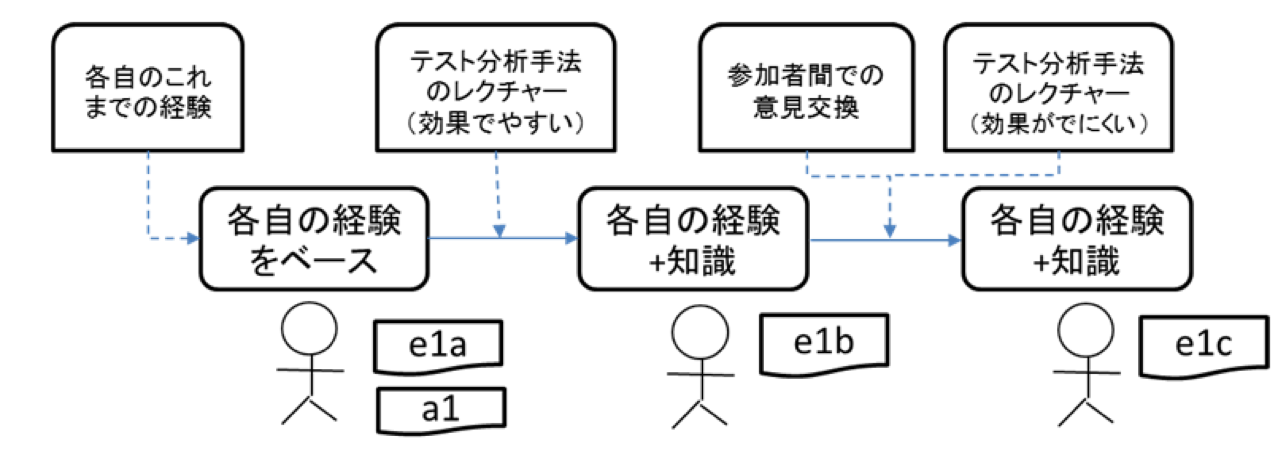
\includegraphics[width=10cm]{./image/D-3-Fig8.png}
\caption{e1aからe1cまでの演習の前提条件の変化}
\label{fig:D-3-Fig8}
\end{center}
\end{figure}
ワークショップを通して,図~\ref{fig:D-3-Fig8}のように,テスト分析手法を知らない状態での演習実施(1a),
一部分だけ説明した状態で演習実施(1b),
全てを説明した状態で演習実施を(1c)行い,各参加者の演習結果を実験データとして収集した.

テスト分析手法のレクチャーを2 回に分けた理由は, 前述したように手法の実施手順がデータフローを使った手順とそれ以外の手順に分けられるため, 2 段階にわけることがワークショップの参加者にとって知識習得が容易になるであろうという判断からである.

\begin{figure}[h]
\begin{center}
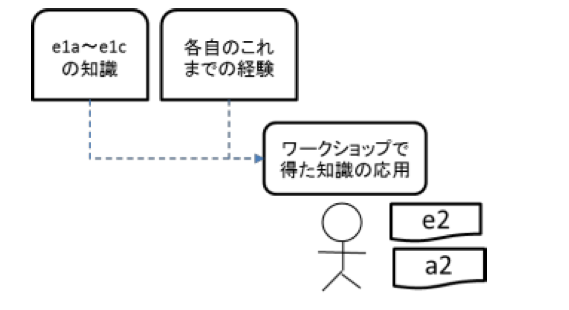
\includegraphics[width=9cm]{./image/D-3-Fig9.png}
\caption{e2 の演習の前提条件の変化}
\label{fig:D-3-Fig9}
\end{center}
\end{figure}
e2 では,図~\ref{fig:D-3-Fig9}のように,e1a からe3a までで行ったレクチャーと演習を通じて得た知識とスキルが別の題材で活用できることを確認する. e1a と比較することで, スキルが向上しているかを観察する.
%すべて説明した状態で演習実施(1c)を行い,各参加者の演習結果を実験データとして収集した.

このワークショップでは,57名分のIT技術者が参加した.
参加者の年齢,業務領域,経験年数とテスト技法の知識は図~\ref{fig:D-3-Fig6},図~\ref{fig:D-3-Fig7},図~\ref{fig:D-3-Fig7b}のとおりである.
年齢構成,業務領域ともに偏りがなく,産業界のサンプリングとして意味があると考える.

\begin{figure}[H]
\begin{center}
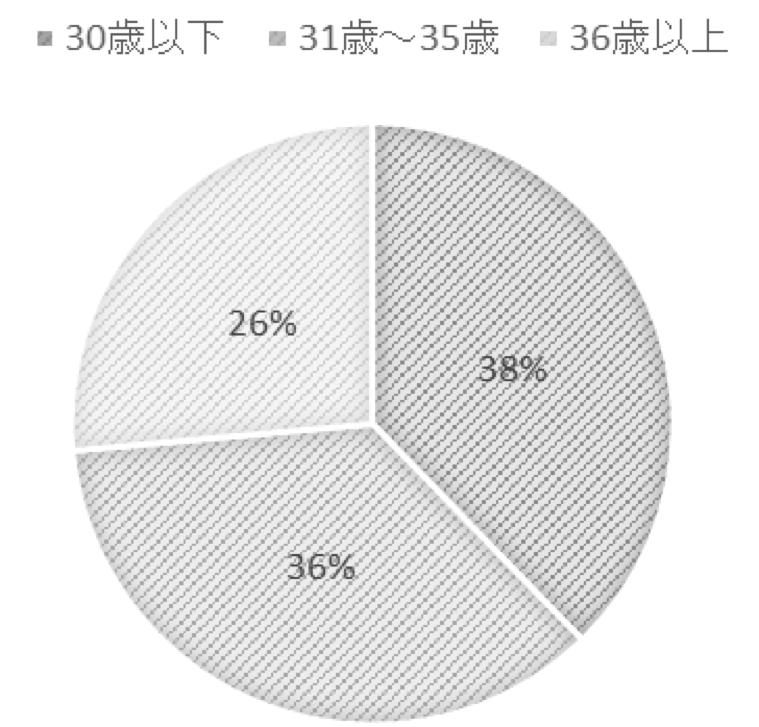
\includegraphics[width=8cm]{./image/D-3-Fig6.png}
\caption{参加者の年齢分布}
\label{fig:D-3-Fig6}
\end{center}
\end{figure}

\begin{figure}[H]
\begin{center}
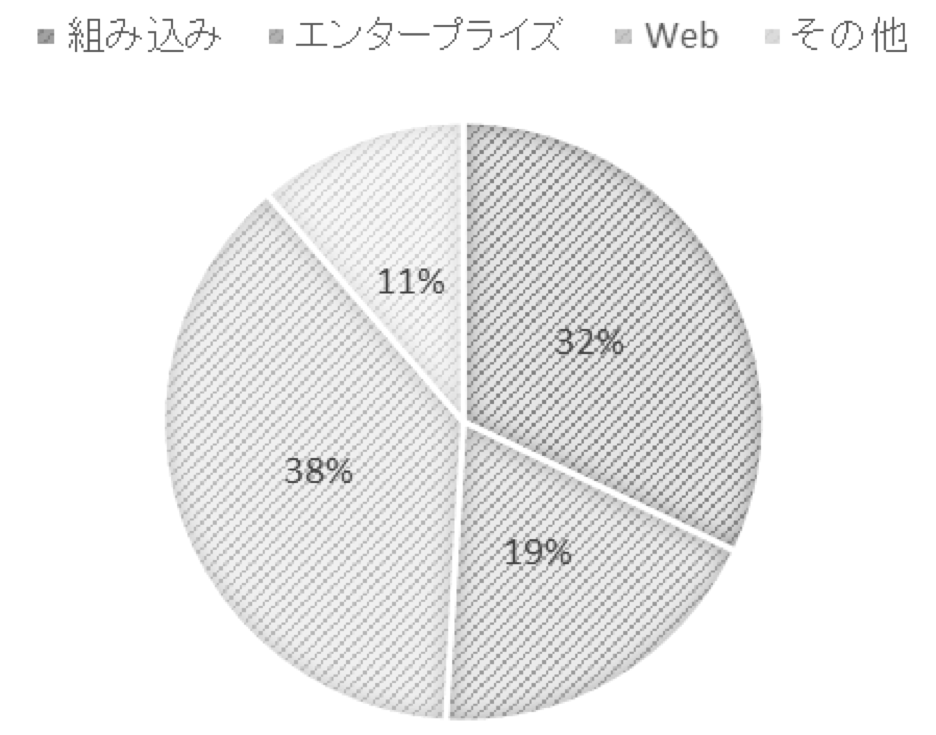
\includegraphics[width=10cm]{./image/D-3-Fig7.png}
\caption{参加者の業務領域分布}
\label{fig:D-3-Fig7}
\end{center}
\end{figure}

参加者の技術経験と,テスト技法の研修受講有無(テスト技法に関する知識習得)については,記述式の調査紙にて確認を行った.
テスト技法の研修受講経験のある技術者が38人と半分以上をしめているのが,いままでの実験の被験者とは異なる.
このワークショップ参加者の特徴として,今までに何らかの研修を受けた経験が一般的な技術者と比較して多いことがあげられる.
この理由は,このワークショップは実費を参加者自身が支払い,土日を費やして実施するものであるためで,参加者のキャリア意識が高いことにある.

\begin{figure}[H]
\begin{center}
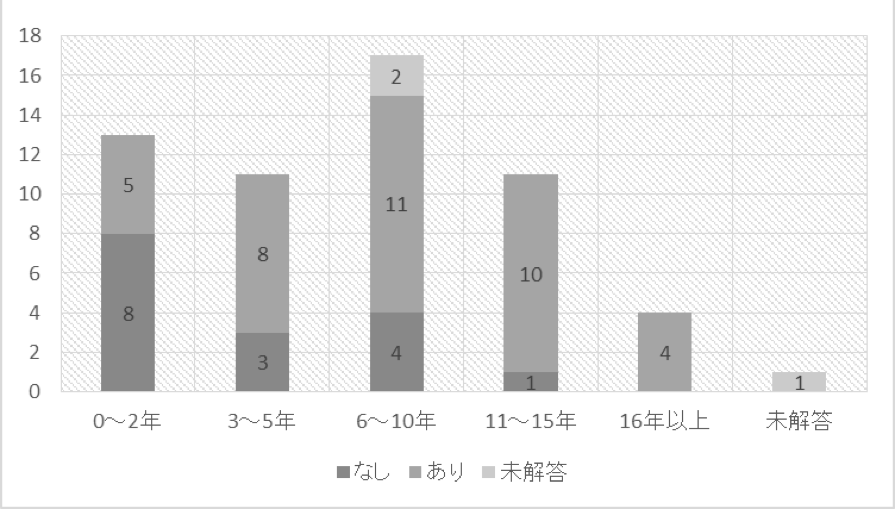
\includegraphics[width=10cm]{./image/D-3-Fig7b.png}
\caption{実務経験とテスト技法研修受講実績}
\label{fig:D-3-Fig7b}
\end{center}
\end{figure}



\subsection{実験の題材}
演習題材は,組み込みソフトウェア開発とエンタープライズシステム開発のシステムレベルの仕様を用意した.
組み込みソフトウェア開発の演習題材は音楽再生用機器の音声コントロールをテスト対象のフィーチャとしたものである.3.2節の[グループ単位1]の演習で利用した題材と同じものである.
エンタープライズシステム開発の演習題材は,フライト予約システムの新規フライト予約をテスト対象のフィーチャとして演習問題を用意した.3.2節の[グループ単位2]の演習で利用した題材と同じものである.
講師側が用意した解答例である,テスト分析で特定すべきテスト条件の一覧は,3.2節同様に表~\ref{tab:D-3-ensyu1}と表~\ref{tab:D-3-ensyu2}となる.


\subsection{実験結果の評価} \label{sec:3-2}
e1a,e1b,e1c,e2 の演習結果において,各参加者が特定できたテスト条件数 (回答数) を図~\ref{fig:D-3-Fig10}の箱ひげ図を用いて比較する.
図~\ref{fig:D-3-Fig10}のY軸は回答したテスト条件数を示し,X 軸は,各演習における回答数の分布を箱ひげ図で示している.

%箱ひげ図 %<図7 参加者あたりのテスト条件特定数>
\begin{figure}[htbp]
  \begin{center}
  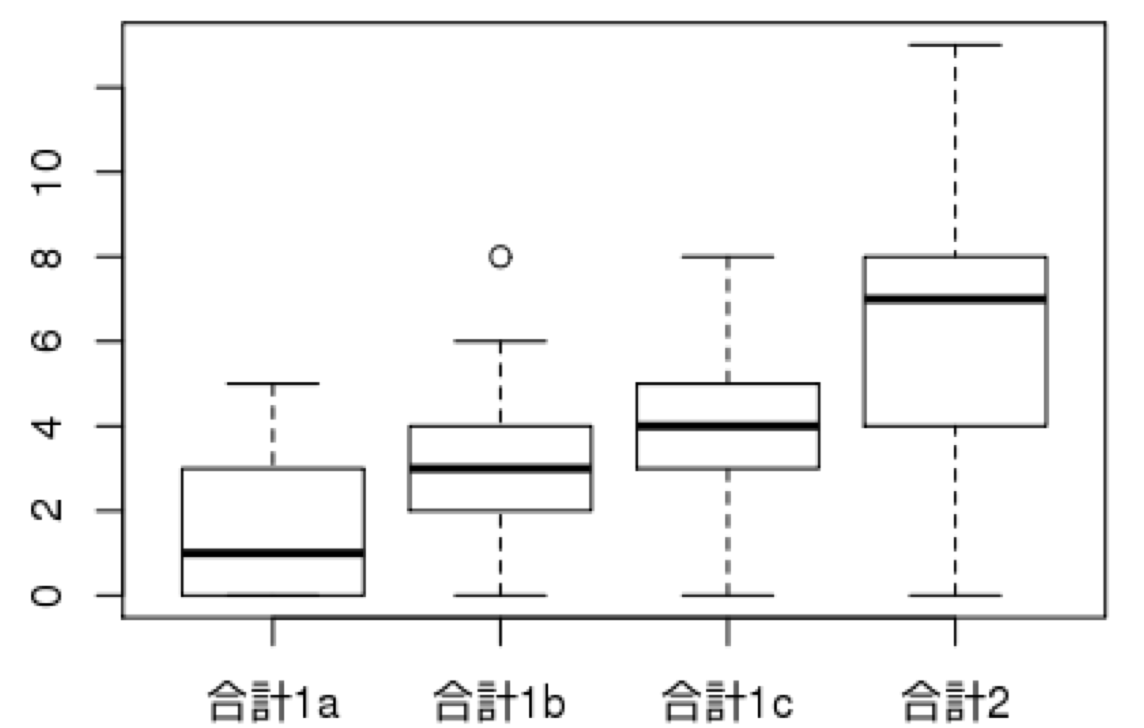
\includegraphics[width=10cm]{./image/D-3-Fig10.png}
  \caption{参加者あたりのテスト条件特定数}
  \label{fig:D-3-Fig10}
  \end{center}
\end{figure}

e1aでは,最高点は5であり,中央値は1 であった.
正解数とした数は9なので,非常に低い値であった.
レクチャー後のe1bでは中央値が3,e1c では4,e2 では7 と,演習が進むごとに中央値が増えているので,テスト条件数を特定するスキルが向上したと考えられる.
ただし,e2 とそれ以外は演習題材が異なり,正解とした条件数が異なる(e2 は23 で,それ以外は9 である).
そのため,単純な数値の比較では不十分である.
正解とするケース数を100 とした箱ひげ図を図~\ref{fig:D-3-Fig11}に示す.
%<図8 参加者あたりのテスト条件特定割合>
\begin{figure}[htbp]
  \begin{center}
  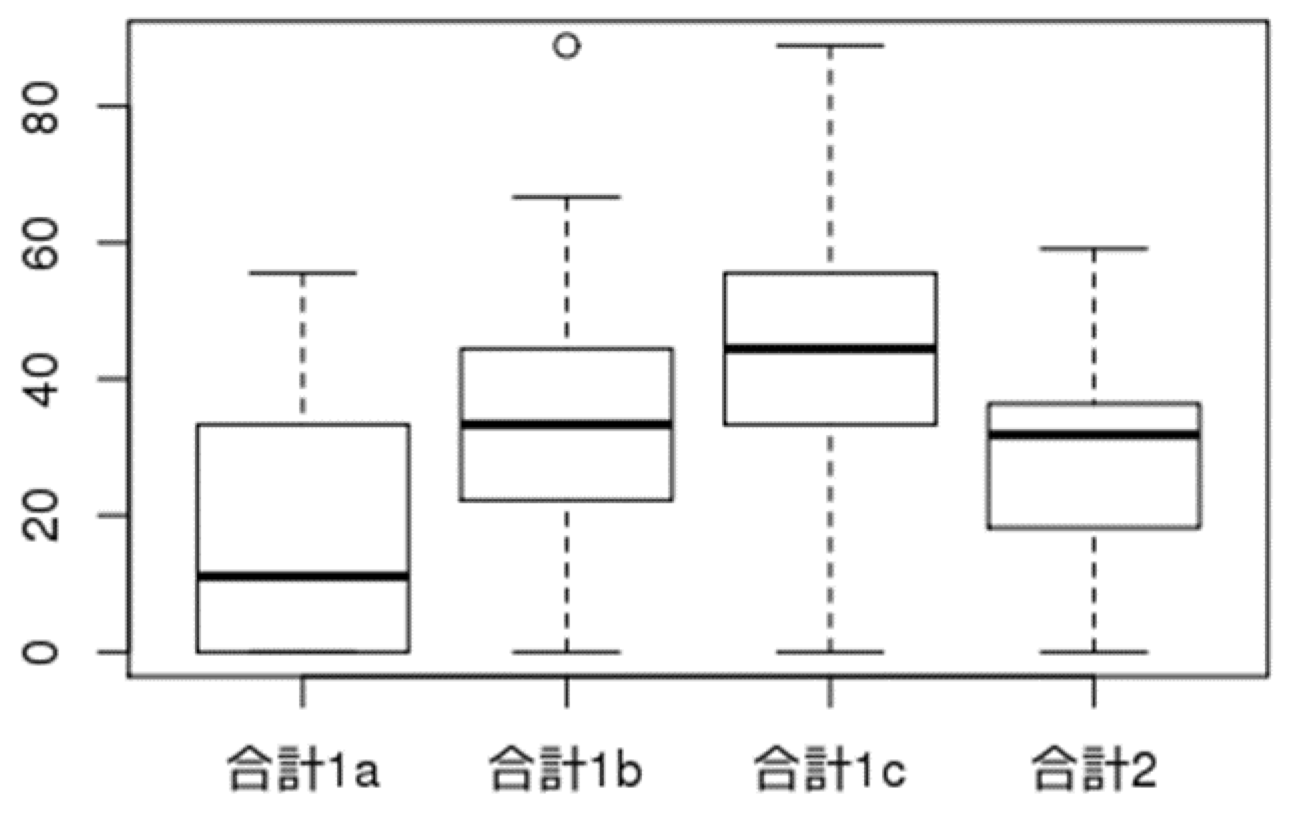
\includegraphics[width=10cm]{./image/D-3-Fig11.png}
  \caption{参加者あたりのテスト条件特定割合}
  \label{fig:D-3-Fig11}
  \end{center}
   \end{figure}

図~\ref{fig:D-3-Fig11}からは, e1a では約10パーセントであったテスト条件の特定数の割合の中央値が,e2 では約40パーセントまで向上したことが確認できる.
ただし,図~\ref{fig:D-3-Fig10}と図~\ref{fig:D-3-Fig11}からわかるように参加者全員のテスト条件特定数が一律に上がったわけではない.
効果があった部分とそうでない部分がどこであるかを調べるために,テスト条件ごとの特徴,および参加者の特徴でさらに分析をすすめた.

\begin{figure}[htbp]
  \begin{center}
  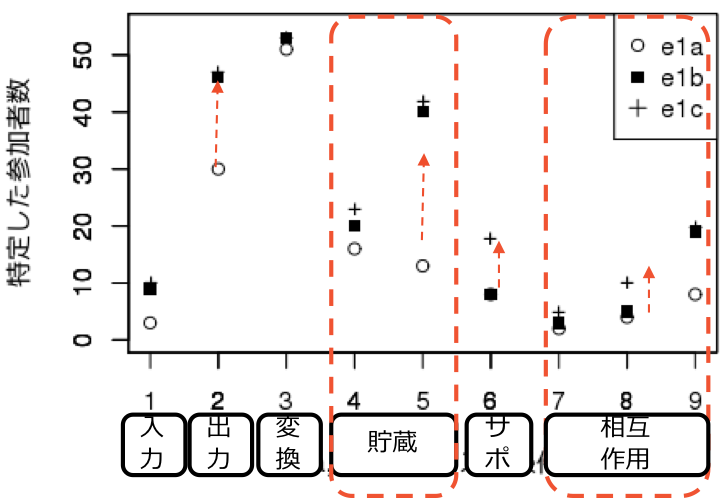
\includegraphics[width=7cm]{./image/D-3-Fig12-1.png}
  \caption{e1aからe1cまでの演習回答の分布}
  \label{fig:D-3-Fig12-1}
  \end{center}
\end{figure}
各参加者が特定できたテスト条件数 (回答数) を図\ref{fig:D-3-Fig12-1}のように論理的機能構造で分類して比較した.
図\ref{fig:D-3-Fig12-1}のY軸はテスト条件毎に解答できた参加者数を示し,X軸は,テスト条件を示している.
1a,1b,1c と進むにつれて,分析で特定できるテスト条件が増えていることがわかる.
テスト分析手法の知識を与えることで特に伸びたのは,出力と貯蔵に属するテスト条件であった.

\begin{table}[htbp]
  \footnotesize
  \centering
  \caption{e1a からe1c までの演習結果の変化表}
    \begin{tabular}{rrrrr}
    \hline
    \multicolumn{1}{|l|}{} & \multicolumn{1}{p{6em}|}{\textbf{論理的機能構造}} & \multicolumn{1}{p{6em}|}{\textbf{テストカテゴリ}} & \multicolumn{1}{p{6em}|}{\textbf{難しさ}} & \multicolumn{1}{p{6em}|}{\textbf{効果}} \bigstrut\\
    \hline
    \multicolumn{1}{|l|}{1} & \multicolumn{1}{p{6em}|}{入力調整} & \multicolumn{1}{p{6em}|}{ボタン} & \multicolumn{1}{p{6em}|}{難} & \multicolumn{1}{p{6em}|}{中} \bigstrut\\
    \hline
    \multicolumn{1}{|l|}{2} & \multicolumn{1}{p{6em}|}{出力調整} & \multicolumn{1}{p{6em}|}{音声出力} & \multicolumn{1}{p{6em}|}{中} & \multicolumn{1}{p{6em}|}{高} \bigstrut\\
    \hline
    \multicolumn{1}{|l|}{3} & \multicolumn{1}{p{6em}|}{変換} & \multicolumn{1}{p{6em}|}{音量} & \multicolumn{1}{p{6em}|}{易} & \multicolumn{1}{p{6em}|}{低} \bigstrut\\
    \hline
    \multicolumn{1}{|l|}{4} & \multicolumn{1}{l|}{\multirow{2}[4]{*}{貯蔵}} & \multicolumn{1}{p{6em}|}{設定保存1} & \multicolumn{1}{p{6em}|}{難} & \multicolumn{1}{p{6em}|}{中} \bigstrut\\
\cline{1-1}\cline{3-5}    \multicolumn{1}{|l|}{5} & \multicolumn{1}{l|}{} & \multicolumn{1}{p{6em}|}{設定保存2} & \multicolumn{1}{p{6em}|}{難} & \multicolumn{1}{p{6em}|}{高} \bigstrut\\
    \hline
    \multicolumn{1}{|l|}{6} & \multicolumn{1}{p{6em}|}{サポート} & \multicolumn{1}{p{6em}|}{状態遷移} & \multicolumn{1}{p{6em}|}{難} & \multicolumn{1}{p{6em}|}{中} \bigstrut\\
    \hline
    \multicolumn{1}{|r|}{7} & \multicolumn{1}{l|}{\multirow{3}[6]{*}{相互作用}} & \multicolumn{1}{p{6em}|}{対向機反映} & \multicolumn{1}{p{6em}|}{難} & \multicolumn{1}{p{6em}|}{低} \bigstrut\\
\cline{1-1}\cline{3-5}    \multicolumn{1}{|r|}{8} & \multicolumn{1}{l|}{} & \multicolumn{1}{p{6em}|}{設定情報共有1} & \multicolumn{1}{p{6em}|}{難} & \multicolumn{1}{p{6em}|}{中} \bigstrut\\
\cline{1-1}\cline{3-5}    \multicolumn{1}{|r|}{9} & \multicolumn{1}{l|}{} & \multicolumn{1}{p{6em}|}{設定情報共有2} & \multicolumn{1}{p{6em}|}{難} & \multicolumn{1}{p{6em}|}{中} \bigstrut\\
    \hline
    \multicolumn{5}{p{30em}}{難しさ 0-10難 11-25中 26-易} \bigstrut[t]\\
    \multicolumn{5}{p{30em}}{0-10低 11-25中 26-高} \bigstrut[t] \\
    \end{tabular}%
  \label{tbl:D-3-tbl10}%
\end{table}%

表~\ref{tbl:D-3-tbl10}は,1から9までのテスト条件を対応する論理的機能構造とテストカテゴリを示し,難しさと教育効果を示した.
難しさは,正解数の分布から3段階に分けた.教育効果は,e1a(教育前)とe1c(教育後)の差を3段階で分類した.
表~\ref{tbl:D-3-tbl10}から,テスト条件2の音声出力と,テスト条件5の設定保存は,演習が進むにつれテスト条件が特定できた参加者が増加したため,特に効果が高かったといえる.これは,過去の実験と同様の結果である.2章にて,仕様書には明確に記述がないものは,テストカテゴリのようなガイドを使うことで特定が容易になるのと仮説をたてて実験を行ったが,今回の実験でもその仮説を実証する結果となった.

続いて,ワークショップ参加者の業務経験年数ごとに,テスト条件を特定できた数にどのような傾向があるかを調査した.ワークショップ参加者の実業務の経験年数はa1でのアンケート結果を利用した.図~\ref{fig:D-3-Fig15}のように,e1aでは,業務経験1~2年の参加者以外は,全ての経験年数で中央値がほぼ同じになった.テスト分析に関して,入社3年でほぼ同様の能力になり,その後は業務経験を重ねてもテストケースを作る能力はあまり変化していない.
入社1~2年では,テスト設計技術に関するスキルの伝達がなされていない,もしくは行われていても効果が出ていないことが推定できる.
%箱ひげ図 %<図7 参加者あたりのテスト条件特定数>
\begin{figure}[htbp]
  \begin{center}
  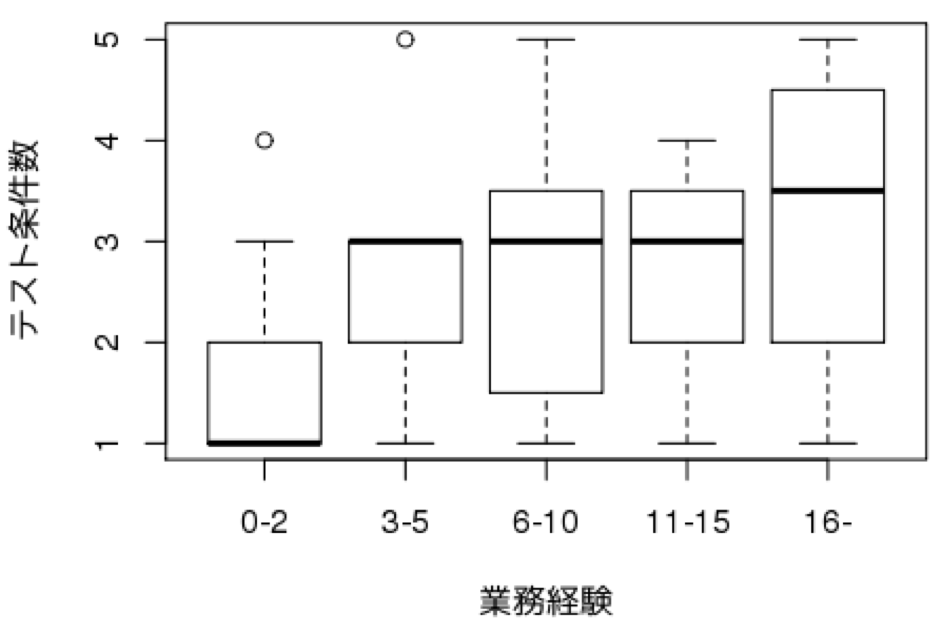
\includegraphics[width=10cm]{./image/D-3-Fig15.png}
  \caption{e1aの参加者/業務経験別テスト条件特定数}
  \label{fig:D-3-Fig15}
  \end{center}
\end{figure}

レクチャーと演習を通じて得たスキルを確認するため,e2aの結果を比較したものが図~\ref{fig:D-3-Fig16}である.全体的に向上しているが,特に業務経験が0-2年度の参加者が伸びたため,業務経験とテスト条件を特定できる能力に差がほとんどなくなってきていることが確認できた.

\begin{figure}[htbp]
  \begin{center}
  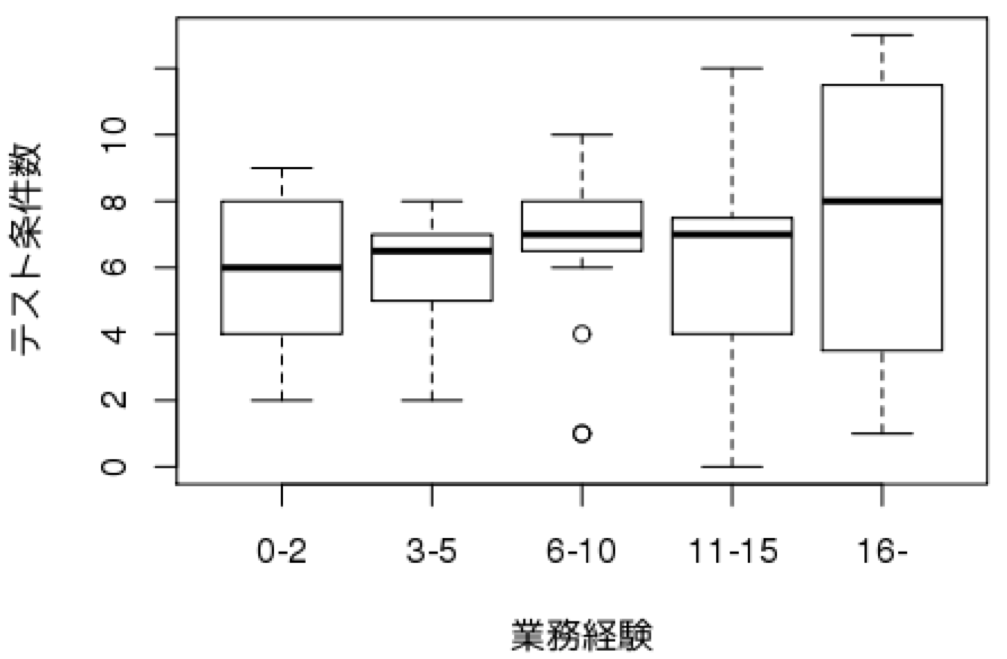
\includegraphics[width=10cm]{./image/D-3-Fig16.png}
  \caption{e2の参加者/業務経験別テスト条件特定数}
  \label{fig:D-3-Fig16}
  \end{center}
   \end{figure}


\subsection{テスト分析手法適用前のテスト分析方法の分類}
今回のワークショップでは, e1aの演習にて,テスト分析結果をこれまでの業務経験に基づいて自由に書いてもらうようにした.
テスト分析手法の知識を与える前のときのテスト分析結果から,テスト分析結果の記載は,図\ref{tbl:D-3-tbl11}に示す通り4つに分類できることがわかった.
%<表3 テスト記述パターン>
% Table generated by Excel2LaTeX from sheet 'Sheet4'
\begin{table}[htbp]

  \centering
  \caption{テスト記述パターン}
    \begin{tabular}{|c|p{9em}|p{14em}|p{3em}|}
    \hline
          & パターン & 記載内容 & \multicolumn{1}{c|}{分類} \bigstrut\\
    \hline
    \hline
    1     & 仕様項目  & 「○○な場合に××なること」といったテスト対象の仕様 & 分析的 \bigstrut\\
    \hline
    2     & テストケース & 入力値,アクション,期待結果 & 実装的 \bigstrut\\
    \hline
    3     & P-V(パラメータ/値) & パラメータと値 & 分析的 \bigstrut[t]\\
    \hline
    4     & シナリオ  & 操作手順として記載 & 実装的 \bigstrut[b]\\
    \hline
    \end{tabular}%
  \label{tbl:D-3-tbl11}%
\end{table}%

表~\ref{tbl:D-3-tbl11}の1と3は中間成果物的であり,記載した内容を見てそのままテストを実行するには不向きであるが,2と4 はそのままテスト実行時に利用できる.
一方,分析や設計をすると1と3が成果物になる.
自由に記載してもらう際に分析結果から書くことは,普段の業務でも分析や設計をしていると想定できる.
ここから2と4 を直接書くのは,普段の業務であまり分析や設計行為をしていないのではないかという仮説をたてた.
普段から業務にて分析や設計をしている参加者のほうが,分析,設計の活動に慣れているために知識の習得が早いと仮定し,今回のワークショップを通じた演習結果にてこれまでの記載方法と演習の成果に相関があるかを調査した.

\begin{figure}[h]
  \begin{center}
  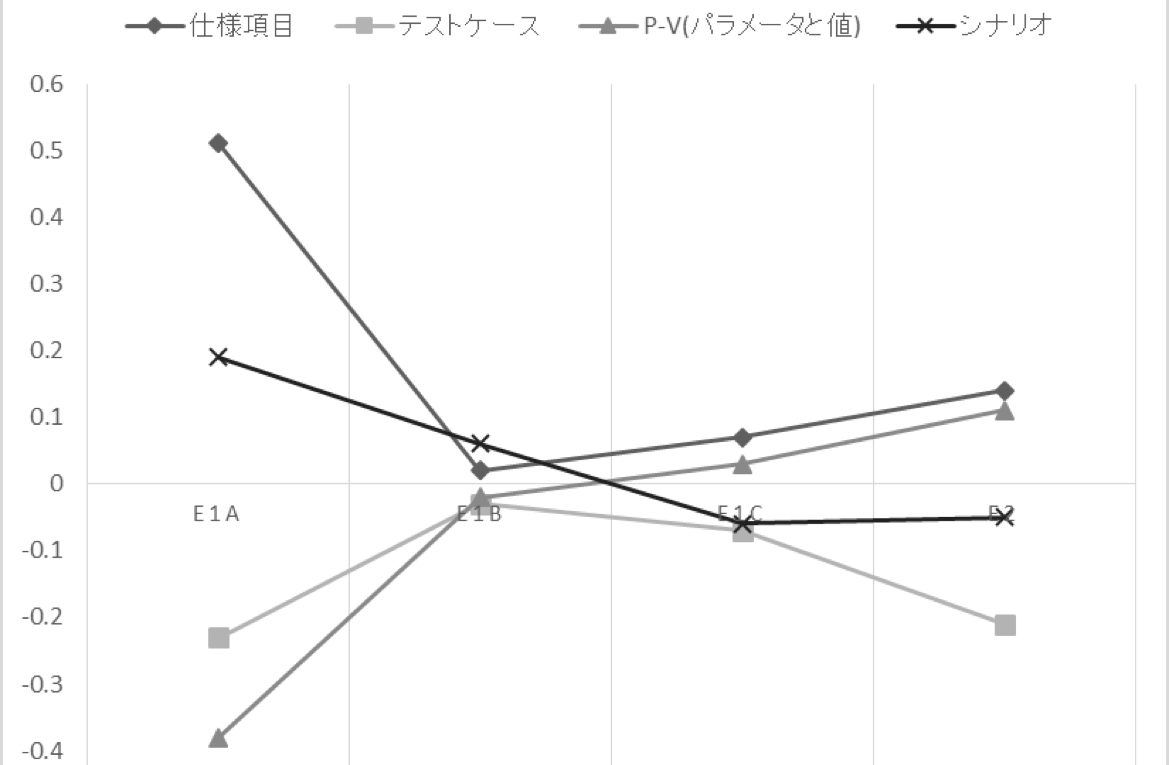
\includegraphics[width=10cm]{./image/D-3-Fig13.png}
  \caption{e1aの参加者業務分野別テスト条件特定数}
  \label{fig:D-3-Fig13}
  \end{center}
\end{figure}

図~\ref{fig:D-3-Fig13} がスピアマンの順序相関分析をした結果である,e1aでは,仕様項目から記載する参加者と特定できたテスト条件数には,0.51(0.4 以上の値は相関ありといえる)の相関が出たたがそれ以外は0.4 以上の値は出なかった.
グラフの傾向からは,e2では分析的な記述をしていた参加者のほうが実装的な記述をした参加者より正の相関となったが,分析結果の値は0.2を割り込んでいるため,相関があるとは結論付けられない.

e1a の仕様項目を記載する参加者だけ相関が出たのは,今回の演習で特定するテスト条件が仕様項目そのものであるため,最初の演習では仕様項目を記載した参加者と結果の相関が出たと考えられる.

\newpage
\section{まとめ}
本章は,3回の予備実験を通して,テスト分析手法を適用する前のテスト分析での結果のばらつきの傾向,及びばらつきの傾向と分析手法を適用後の結果との相関を調査した.
実験はワークショップを通じてグループ単位で2回,個人単位で1回行なった.
テスト対象を詳細化するときに分類に対する一貫性が欠如していることによるテスト分析結果のばらつきを確認することができた.
また,分類していくルールとしてテストカテゴリベースドテストの知識を与えることで,テスト条件を特定できる数が増えることが確認できた.仮説として立てた「仕様書には明確に記述がないものは,テストカテゴリのようなガイドを使うことで特定が容易になる」ことが実証できる傾向になった.
ただし,テストカテゴリベースドテストの知識を与えても期待した数のテスト条件を特的できるわけではないことがわかった.
また,業務経歴3年未満の技術者には有効であったが,3年以上の技術者にはあまり効果がないこともわかった.

%%%%%%%%%%%%%%%%%%%%%%%

%%%%%%%%%%%%%%%%%%%%%%%InSTA2015の論文
\chapter{I/O テストデータパターンによるテストケース抽出手法}\label{chap:4}
本章では,テスト分析において,テスト条件を網羅的に特定する方法として,テスト実行時のデータの入出力(以降I/Oと呼ぶ)に着目する.
テストベースを分析する際に,テスト実行時のI/Oの要素で分析を進めることで,網羅的にテスト条件を特定する方法を提案する.
3章の題材を使って提案手法の適用評価を行う.
また,現実に使われたモバイルアプリケーション開発プロジェクトのテストケースを入手し,そのテストケースとI/Oテストデータパターンを使って特定したテスト条件の内容を比較し,手法を適用することで特定できるテスト条件にどのようなものがあるかを確認する.

\newpage
\section{I/Oテストデータパターンの概要} \label{sec:4-1}
\subsection{テストカテゴリベースドテストの課題} \label{sec:4-1-1}
3章の実験を通して,テストカテゴリベースドテストの適用に一定の効果は確認できたものの,
知識を与えても期待した数のテスト条件を特定できるわけではないことがわかった.
また,業務経歴3年未満の技術者には有効であったが,3年以上の技術者にはあまり効果がないこともわかった.
テストカテゴリベースドテストは,テストベースの分析に論理的機能構造をガイドとして使用することを明示しているだけであり,具体的な分析手順について定義できていない.
本章では,テスト条件を網羅的に特定する方法として,テスト実行時のデータのI/Oに着目する方法を提案する.
提案する手法が適用可能であることを評価し,手法を適用することにって適用前では特定できなかったテスト条件が
特定できるようになることを現実に使われたモバイルアプリケーション開発プロジェクトのテストケースとの比較で評価する,

\subsection{I/Oテストデータパターン} \label{sec:4-1-1}
テストを実行するためには,テスト対象となる$AS$のタスク$Ta$に対して,源泉$So$からデータを入力し,$Ta$から$So$へ出力されたデータと期待結果とを比較する.

たとえば,シンプルな機能の四則演算の計算結果が正しいことを検証するときには,$AS$の外部となる源泉$So_i$から計算の対象となる複数の値$In_i$を入力し,タスク$Ta_i$がそれらの値を計算し,計算結果$Out_i$をテスト対象の外部である$So_i$へ出力する.

これは図~\ref{fig:D-3-Fig4}で示している「外部からのデータ入力,外部へのデータ出力」というパターンになる.また,$So_j$から入力する数値$In_j$に対して,保持データ$Ds_j$である固定比率を使って計算を行う場合,$Ta_j$は$Ds_j$を呼び出し,計算にその値を利用してから計算結果$Out_j$を$So_j$へ出力する.
これは図~\ref{fig:D-3-Fig4}で示している例「外部と内部からのデータ入力,外部へのデータ出力」となる.
\begin{figure}[htbp]
 \begin{center}
 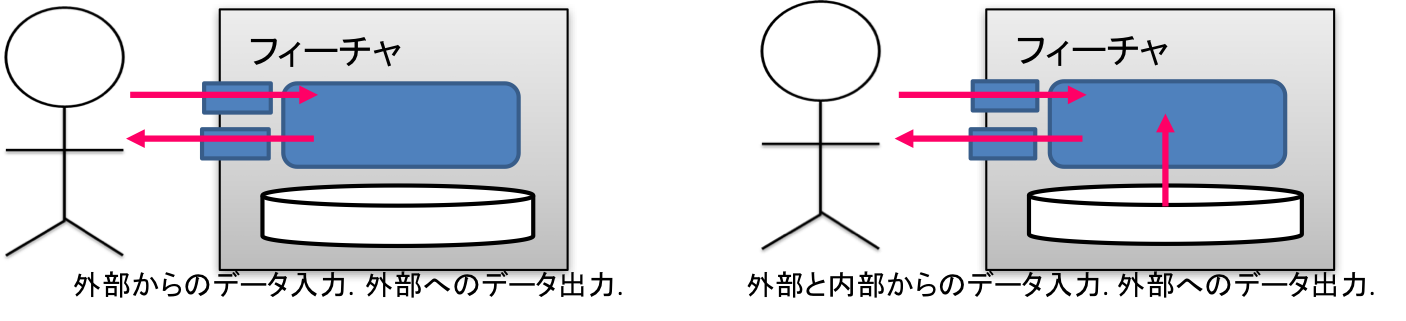
\includegraphics[width=12cm]{./image/D-3-Fig4.png}
 \caption{テスト対象へのデータ入出力の説明}
 \label{fig:D-3-Fig4}
 \end{center}
\end{figure}

テスト実行をするときの$Ta$へのデータ$In$のパターンは,外部からの入力,内部に保持したデータの入力,外部と内部からの入力の3パターンに分類できる.
同じようにテスト対象からのデータ$Out$のパターンは外部への出力,内部に保持したデータの出力,外部と内部からデータの出力の3パターンに分類できる.
これらテスト対象に対するテスト実行時のデータの入出力をまとめたパターンは図~\ref{fig:D-4-Fig6}のように9パターンに集約できる.

\begin{figure}[htbp]
\begin{center}
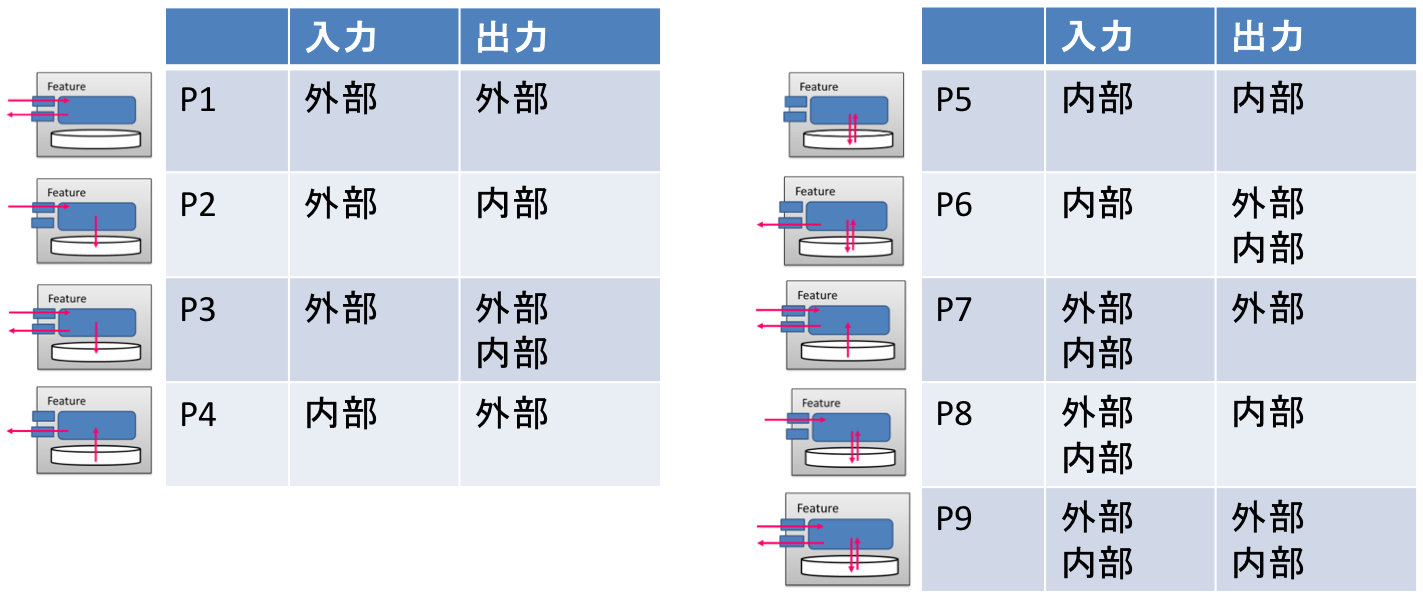
\includegraphics[width=14cm]{./image/D-3-Fig5.png}
\caption{I/Oテストデータパターン}
\label{fig:D-4-Fig6}
\end{center}
\end{figure}

これをI/Oテストデータパターンと呼ぶ.
I/Oテストデータパターンがテスト実行時のデータの入出力から見た全体集合となる.

Whittakerによって提案されているフォールトモデル\cite{whittaker2003break}は,$AS$の$Ta$に対する$In$と$Out$のモデルに関する類似の研究である.
フォールトモデルの目的はフォールトを見つけることであり,I/Oテストデータパターンで提示しているデータの入出力モデルはテストベースからテスト条件の中の仕様項目を特定するためのモデルとして使われる.


注意すべきこととしてI/Oテストデータパターンはテスト対象の外部からの観察が可能なものを選ぶことがあげられる.
$Ta$の起動終了に使われる内部のコマンド(シグナルやイベント)は,データパターンへ分類をするときに考慮しない.
なぜならこの手法はブラックボックステストのためのテストベースの分析手法であり,$AS$内部のシグナルやイベントのような外部観察ができないコマンドは,システムテストレベルでのブラックボックステストでは,明示的に考慮できないからである.

テスト分析で特定した仕様項目は,テスト実行をした際の入出力にて確認することができなければならないので,すべてが9パターンのどれかに分類できると考えられる.

\subsection{テストカテゴリベースドテストとの関係}

P1からP9のI/Oテストデータパターンは,単一の$Ta$に対するデータ入出力の全体像となる.
テスト実行の際,$So$から入力を行い,$So$へ出力する間に,データは,テスト対象となる$Ta$によって論理的機能構造の入力調整,出力調整,変換,貯蔵を通過する.
I/OテストデータパターンのP1からP9のそれぞれが論理的機能構造のどの要素に該当するかを表~\ref{tbl:D-4-tbl1}にまとめた.

% Table generated by Excel2LaTeX from sheet 'Sheet3'
\begin{table}[htbp]
  \centering
  \caption{I/Oテストデータパターンと論理的機能構造}
    \begin{tabular}{|r|p{4em}|l|l|l|p{4em}|l|l|}
    \hline
          & \multicolumn{1}{l|}{} & \multicolumn{1}{p{4em}|}{\textbf{入力調整}} & \multicolumn{1}{p{4em}|}{\textbf{出力調整}} & \multicolumn{1}{p{4em}|}{\textbf{変換}} & \textbf{貯蔵} & \multicolumn{1}{p{2em}|}{\textbf{サポート}} & \multicolumn{1}{p{1.915em}|}{\textbf{相互作用}} \bigstrut\\
    \hline
    \multicolumn{1}{|p{1.5em}|}{\textbf{入力}} & \textbf{外部} & \multicolumn{1}{p{4em}|}{P1,P2,P3} &       & \multicolumn{1}{p{4em}|}{P1,P2,P3} & \multicolumn{1}{l|}{} &       &  \bigstrut\\
\cline{2-8}          & \textbf{内部} &       &       & \multicolumn{1}{p{4em}|}{P4,P5,P6} & P4,P5,P6 &       &  \bigstrut\\
\cline{2-8}          & \textbf{外部と内部} & \multicolumn{1}{p{4em}|}{P7,P8,P9} &       & \multicolumn{1}{p{4em}|}{P7,P8,P9} & P7,P8,P9 &       &  \bigstrut\\
    \hline
    \multicolumn{1}{|p{1.5em}|}{\textbf{出力}} & \textbf{外部} &       & \multicolumn{1}{p{4em}|}{P1,P4,P7} &       & \multicolumn{1}{l|}{} &       &  \bigstrut\\
\cline{2-8}          & \textbf{内部} &       &       &       & P2,P5,P8 &       &  \bigstrut\\
\cline{2-8}          & \textbf{外部と内部} &       & P3,P6,P9 &       & P3,P6,P9 &       &  \bigstrut\\
    \hline
    \end{tabular}%
  \label{tbl:D-4-tbl1}%
\end{table}%


P1に分類できるシンプルな四則演算を行う$Ta$の場合,外部からの入力に対して外部に出力する間に,
図~\ref{fig:D-4-Fig7}のように論理的機能構造の入力調整,変換,出力調整を通過する.
そのため,P1は,表~\ref{tbl:D-4-tbl1}の以下の3箇所にプロットされている.
\begin{itemize}
  \item 列:入力調整 行:入力/外部
  \item 列:出力調整 行:出力/外部
  \item 列:変換 行:入力/外部
\end{itemize}

このデータフローで通過する3箇所が,P1の場合の期待結果を確認する候補となる.
これらを本研究ではチェックポイントと呼ぶ.
チェックポイントのうち,期待結果を意図的に確認する必要があると判断したものがテスト分析で特定すべき仕様項目,つまりテスト条件となる.

 \begin{figure}[htbp]
 \begin{center}
 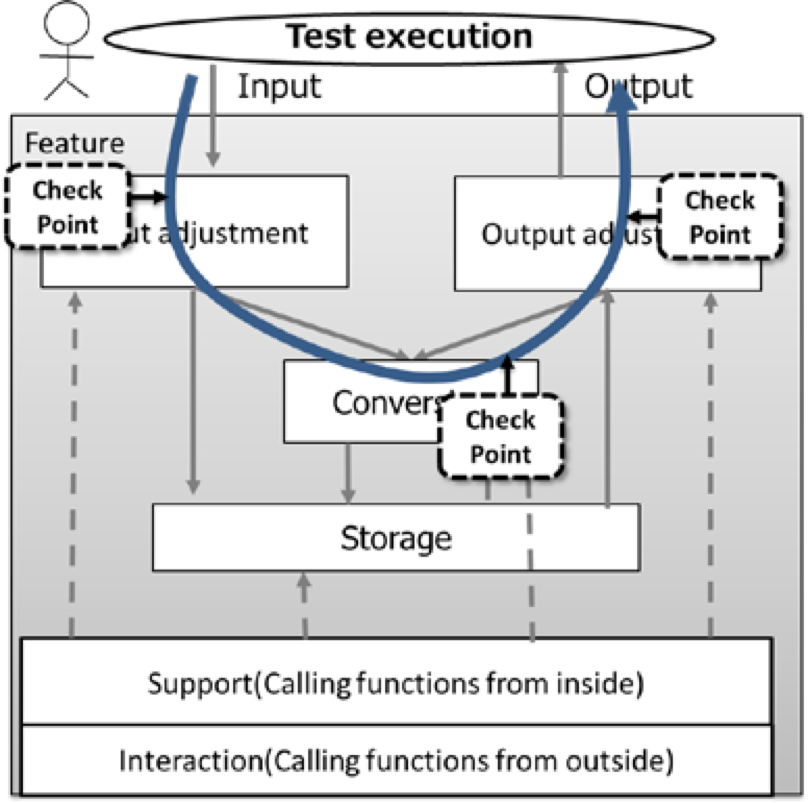
\includegraphics[width=10cm]{./image/D-4-Fig7.png}
 \caption{I/Oテストデータパターンのデータの流れ}
 \label{fig:D-4-Fig7}
 \end{center}
 \end{figure}

データフローの中で通過する3箇所のチェックポイントのうち,少なくとも1つのチェックポイントをテスト条件として特定するが,全てが実際に期待結果を確認する仕様項目になるとは限らない.
例えば,テストすべき仕様項目を特定する際に,入力調整に該当する入力の際に適切な値だけ受け入れることと,変換に該当する計算が適切に行われていることはテストすべきであるが,出力調整が適切にされることは,すでに自明であるためにテストケースとする必要がないということが考えられるためである.

また,表~\ref{tbl:D-4-tbl1}では,サポートと相互作用についてはデータパターンがプロットされていない.
P1からP9のI/Oテストデータパターンは,単一の$Ta$に対するデータ入出力の全体像だからである.
論理的機能構造の要素である入力調整,出力調整,変換,貯蔵は,外部観察可能な単一の$Ta$に対するデータ入出力のみを考慮している分類であるのに対して,サポートと相互作用は,単一の$Ta$に対するデータ入出力だけではなく,関係する他の$Ta$の呼び出しに着目して仕様項目を特定するための分類である.

サポートと相互作用に分類される仕様項目は,単一の$Ta$に対するデータの入出力の後,何かしらの方法で呼び出した他の$Ta$の出力で期待結果を確認する.
呼び出されたタスクのI/Oテストデータパターンは,論理的に全パターンが発生する可能性がある.


\newpage
\section{I/Oテストデータパターンの適用評価}
本節では,I/Oテストデータパターンの考え方を,3章で行なったテストカテゴリベースドテストの知識を与える前と後を比較する実験結果を使って適用評価を行う.
最初に,演習にて利用したテスト分析の講師解答例をI/Oテストデータパターンに分類するために,解答例のテスト条件に対して,P1からP9の識別子を属性として付与する.
そして,「3.2節 グループ単位の検証実験からの考察」での実験結果を3章の表~\ref{tbl:D-3-tbl4}で示した評価レベルで整理する.その後,表~\ref{tbl:D-4-tbl1}と同じフォーマットの表に出現結果を当てはめて,これらの題材にてどのI/Oテストデータパターンが現れるのかを確認する.

\subsection{論理的機能構造の適用評価の分析}
グループ単位の検証実験からの考察では,ヘッドセットのフィーチャセットであるボリュームコントロールと,フライト予約システムのフィーチャセットである新規フライト予約の2種類の異なった題材を実験に使用した.
この実験では,被験者のグループがテストカテゴリベースドテストの知識を得ることでテスト条件をどのように多く特定できるようになるかを確認している.
この実験結果をI/Oテストデータパターンにて評価した結果は,表~\ref{tbl:D-4-tbl7}と表~\ref{tbl:D-4-tbl8}に示したとおりである.
前節の結果と本節の結果では行数が異なる理由は, 同じテストカテゴリに属する仕様項目だとしてもデータの入出力が異なるものがあり,場合によってはI/Oテストデータパターンを付与していることがあるためである.例えば,表~\ref{tbl:D-4-tbl7}では,変換が2行あるが,I/OテストデータパターンはP4とP1となることが該当する.
この実験結果からは,表~\ref{tbl:D-4-tbl7}と表~\ref{tbl:D-4-tbl8}が示すとおり, P1, P2, P4, P7 がフィーチャセットに対応するI/Oテストデータパターンとなる.

% Table generated by Excel2LaTeX from sheet 'データの入出力ごとフェリカ (掲載用加工)'
\begin{table}[htbp]
  \centering
\caption{音楽再生機器の演習結果とI/Oテストデータパターン}
    \begin{tabular}{|l|l|l|l|l|l|l|l|}
    \hline
    \multicolumn{2}{|c|}{\multirow{2}[4]{*}{論理的機能構造}} & \multicolumn{6}{c|}{チーム} \bigstrut\\
\cline{3-8}    \multicolumn{2}{|c|}{} & TM1   & TM2   & TM3   & TM4   & TM5   & TM6 \bigstrut\\
    \hline
    \textbf{変換} & P4    & B     & B     & B     & B     & -     & B \bigstrut\\
    \hline
    \textbf{変換} & P1    & B     & A${}^\text{+}$    & B     & B     & B     & - \bigstrut\\
    \hline
    \textbf{出力} & P7    & -     & -     & -     & -     & -     & A${}^\text{+}$ \bigstrut\\
    \hline
    \textbf{貯蔵} & P2    & -     & A${}^\text{+}$    & -     & A${}^\text{+}$    & A${}^\text{+}$    & - \bigstrut\\
    \hline
    \textbf{サポート} & P1    & B     & B     & B     & B     & B     & B \bigstrut\\
    \hline
    \textbf{相互作用} & P1    & B     & A${}^\text{+}$    & A${}^\text{+}$    & A${}^\text{+}$    & A${}^\text{+}$    & A${}^\text{+}$ \bigstrut\\
    \hline
    \textbf{相互作用} & P4    & B     & B     & B     & A${}^\text{+}$    & B     & A${}^\text{+}$ \bigstrut\\
    \hline
    \end{tabular}%
\label{tbl:D-4-tbl7}%
\end{table}%

% Table generated by Excel2LaTeX from sheet 'D論4章用'
\begin{table}[htbp]
  \centering
\caption{フライト予約システムの演習結果とI/Oテストデータパターン}
    \begin{tabular}{|l|l|l|l|}
    \hline
    \multicolumn{2}{|c|}{\multirow{2}[4]{*}{論理的機能構造}} & \multicolumn{2}{c|}{チーム} \bigstrut\\
\cline{3-4}    \multicolumn{2}{|c|}{} & TM1   & TM2 \bigstrut\\
    \hline
    \textbf{変換} & P7    & A     & A \bigstrut\\
    \hline
    \textbf{入力} & P1    & B     & B \bigstrut\\
    \hline
    \textbf{入力} & P7    & A     & - \bigstrut\\
    \hline
    \textbf{入力} & P4    & -     & - \bigstrut\\
    \hline
    \textbf{出力} & P4    & B     & B \bigstrut\\
    \hline
    \textbf{出力} & P4    & A     & A \bigstrut\\
    \hline
    \textbf{出力} & P7    & B     & B \bigstrut\\
    \hline
    \textbf{貯蔵} & P2    & A${}^\text{+}$    & A${}^\text{+}$ \bigstrut\\
    \hline
    \textbf{貯蔵} & P7    & A     & A \bigstrut\\
    \hline
    \textbf{サポート} & P1    & -     & A${}^\text{+}$ \bigstrut\\
    \hline
    \textbf{サポート} & P1    & B     & B \bigstrut\\
    \hline
    \textbf{相互作用} & P4    & B     & A \bigstrut\\
    \hline
    \end{tabular}%
\label{tbl:D-4-tbl8}%
\end{table}%

I/Oテストデータパターンで評価レベルの数を集約した結果が表~\ref{tbl:D-4-tbl9}と表~\ref{tbl:D-4-tbl20}である.
各I/Oテストデータパターンにて A と A${}^\text{+}$ の割合を確認すると,P2のみが音楽再生機器,フライト予約システムの両方の検証実験で100%となっているため,P2のデータパターンに対する効果が最も高いと言える.

音楽再生機器の場合,P2に分類された仕様項目は「ボリューム値の保存」である.
この仕様項目はテストベースに記述はされているものの,ボリュームコントロールのセクションとは別のセクションに記述されている.
飛行機予約システムの場合,P2に分類された仕様項目は注文内容の「データベースへの保存」である.
データベースへの保存に関して,テストベースには,詳しい記載は無い.
これらの観察結果は2章にて述べたテスト条件の特定を困難にしている課題の一つである「明白に必要だと思われる仕様の一部分が記述されていない.」と一致する.

% Table generated by Excel2LaTeX from sheet 'D論4章用'
\begin{table}[htbp]
  \centering
  \caption{I/Oテストデータパターンごとの集計結果}
    \begin{tabular}{lllllr}
    音楽再生機器 &       &       &       &       &  \bigstrut[b]\\
    \hline
    \multicolumn{1}{|c|}{\multirow{2}[4]{*}{I/O パターン}} & \multicolumn{4}{c|}{評価レベル}    & \multicolumn{1}{c|}{\multirow{2}[4]{*}{割合}} \bigstrut\\
\cline{2-5}    \multicolumn{1}{|c|}{} & \multicolumn{1}{l|}{A${}^\text{+}$} & \multicolumn{1}{l|}{A} & \multicolumn{1}{l|}{-} & \multicolumn{1}{l|}{B} & \multicolumn{1}{c|}{} \bigstrut\\
    \hline
    \multicolumn{1}{|l|}{P1} & \multicolumn{1}{r|}{6} & \multicolumn{1}{r|}{0} & \multicolumn{1}{r|}{7} & \multicolumn{1}{r|}{11} & \multicolumn{1}{r|}{35.3\%} \bigstrut\\
    \hline
    \multicolumn{1}{|l|}{P2} & \multicolumn{1}{r|}{3} & \multicolumn{1}{r|}{0} & \multicolumn{1}{r|}{3} & \multicolumn{1}{r|}{0} & \multicolumn{1}{r|}{100.0\%} \bigstrut\\
    \hline
    \multicolumn{1}{|l|}{P4} & \multicolumn{1}{r|}{2} & \multicolumn{1}{r|}{0} & \multicolumn{1}{r|}{1} & \multicolumn{1}{r|}{9} & \multicolumn{1}{r|}{18.2\%} \bigstrut\\
    \hline
    \multicolumn{1}{|l|}{P7} & \multicolumn{1}{r|}{1} & \multicolumn{1}{r|}{0} & \multicolumn{1}{r|}{5} & \multicolumn{1}{r|}{0} & \multicolumn{1}{r|}{100.0\%} \bigstrut\\
    \hline
    \multicolumn{5}{l}{割合 = (A${}^\text{+}$  +  A) /(A${}^\text{+}$  +  A + B) } &  \bigstrut[t]\\
    \end{tabular}%
\label{tbl:D-4-tbl9}%
\end{table}%

% Table generated by Excel2LaTeX from sheet 'D論4章用'
\begin{table}[htbp]
  \centering
  \caption{I/Oテストデータパターンごとの集計結果}
    \begin{tabular}{lllllr}
    フライト予約 &       &       &       &       &  \bigstrut[b]\\
    \hline
    \multicolumn{1}{|c|}{\multirow{2}[4]{*}{I/O パターン}} & \multicolumn{4}{c|}{評価レベル}    & \multicolumn{1}{c|}{\multirow{2}[4]{*}{}} \bigstrut\\
\cline{2-5}    \multicolumn{1}{|c|}{} & \multicolumn{1}{l|}{A${}^\text{+}$} & \multicolumn{1}{l|}{A} & \multicolumn{1}{l|}{-} & \multicolumn{1}{l|}{B} & \multicolumn{1}{c|}{} \bigstrut\\
    \hline
    \multicolumn{1}{|l|}{P1} & \multicolumn{1}{r|}{1} & \multicolumn{1}{r|}{0} & \multicolumn{1}{r|}{1} & \multicolumn{1}{r|}{4} & \multicolumn{1}{r|}{20.0\%} \bigstrut\\
    \hline
    \multicolumn{1}{|l|}{P2} & \multicolumn{1}{r|}{2} & \multicolumn{1}{r|}{0} & \multicolumn{1}{r|}{0} & \multicolumn{1}{r|}{0} & \multicolumn{1}{r|}{100.0\%} \bigstrut\\
    \hline
    \multicolumn{1}{|l|}{P4} & \multicolumn{1}{r|}{0} & \multicolumn{1}{r|}{3} & \multicolumn{1}{r|}{2} & \multicolumn{1}{r|}{3} & \multicolumn{1}{r|}{50.0\%} \bigstrut\\
    \hline
    \multicolumn{1}{|l|}{P7} & \multicolumn{1}{r|}{0} & \multicolumn{1}{r|}{3} & \multicolumn{1}{r|}{1} & \multicolumn{1}{r|}{2} & \multicolumn{1}{r|}{60.0\%} \bigstrut\\
    \hline
    \multicolumn{5}{l}{割合 = (A${}^\text{+}$  +  A) /(A${}^\text{+}$  +  A + B) } &  \bigstrut[t]\\
    \end{tabular}%
\label{tbl:D-4-tbl20}%
\end{table}%

\subsection{I/Oテストデータパターンの出現傾向の調査}

実験にて利用した2つの演習題材に対するテスト分析の講師解答例をI/Oテストデータパターンに分類した結果が表~\ref{tab:addlabel-3}である.
この実験の題材にて使われたI/Oテストデータパターンは,P1とP2とP4とP7の4つであったため,表~\ref{tab:addlabel-3}にはそれらのみを記載している.
またP1としてプロットされているのは入力調整と変換のみであり,出力調整に該当するテスト条件は無かった.
同様にP2としてプロットしているのは貯蔵のみ,P4としてプロットしているのは変換と出力調整のみであり,各I/Oテストデータパターンでは,テスト実行のデータフローの中で期待結果を確認するチェックポイントが限られていることが確認できた.

% Table generated by Excel2LaTeX from sheet 'Sheet3'
\begin{table}[htbp]
  \centering
  \caption{I/Oテストデータパターンの出現傾向の調査結果}
    \begin{tabular}{|r|p{4em}|p{4em}|p{4em}|p{3em}|p{3em}|p{4em}|p{4em}|}
    \hline
          & \multicolumn{1}{l|}{} & \multicolumn{1}{p{4em}|}{\textbf{入力調整}} & \multicolumn{1}{p{4em}|}{\textbf{出力調整}} & \multicolumn{1}{p{4em}|}{\textbf{変換}} & \multicolumn{1}{p{4em}|}{\textbf{貯蔵}} & \multicolumn{1}{p{2em}|}{\textbf{サポート}} & \multicolumn{1}{p{1.915em}|}{\textbf{相互作用}} \bigstrut\\
    \hline
    \multicolumn{1}{|p{1.5em}|}{\textbf{入力}} & \textbf{外部} & P1(F) &       & P1(V) &       &       &  \bigstrut\\
\cline{2-8}          & \textbf{内部} &       &       & P4(V) &       &       &  \bigstrut\\
\cline{2-8}          & \textbf{外部と内部} & \multicolumn{1}{p{4em}|}{P7(F)} &       & \multicolumn{1}{p{4em}|}{P7(F)} & \multicolumn{1}{p{4em}|}{P7(F)} &       &  \bigstrut\\
    \hline
    \multicolumn{1}{|p{1.5em}|}{\textbf{出力}} & \textbf{外部} &       & P4(F)とP7(VF) &       &       & P1(V) & \multicolumn{1}{|p{3em}|}{P1(V), P4(VF)} \bigstrut\\
\cline{2-8}          & \textbf{内部} &       &       &       & \multicolumn{1}{p{4em}|}{P2(VF)} & P2(F) &  \bigstrut\\
\cline{2-8}\cline{8-8}          & \textbf{外部と内部} &       &       &       &       &       &  \bigstrut\\
    \hline
    \end{tabular}%
  \label{tab:addlabel-3}%
\end{table}%

\subsection{サポートと相互作用に関する考察}
前述したように,論理的機能構造の要素の中で,サポートと相互作用は,単一の$Ta$に対するデータの入出力だけではなく,関係する他の$Ta$の呼び出しに着目している.
テスト条件として特定するのは,最初のテストアクションで操作されるタスク$Ta_k$の入出力のデータフローのチェックポイントからではなく,他のタスク$Ta_l$の入出力のデータフローのチェックポイントである.

表~\ref{tbl:D-4-tbl1}では,サポートと相互作用に分類できるI/Oテストデータパターンを特定できていなかったが,実際のテスト分析結果から調査した結果,表~\ref{tab:addlabel-3}で示したとおり,P1とP2とP4にテスト条件を分類した.

表~\ref{tab:D-4-SandI}は,表~\ref{tab:addlabel-3}にてサポートと相互作用に分類したテスト条件の一覧である.

% Table generated by Excel2LaTeX from sheet 'Sheet3'
\begin{table}[htbp]
  \centering
  \caption{サポートと相互作用に分類されたテスト条件一覧}
    \begin{tabular}{|r|p{8em}|p{4em}|p{4em}|p{5em}|}
    \hline
    \multicolumn{1}{|p{4em}|}{\textbf{フィーチャ}} & \textbf{テスト条件} & \textbf{I/Oテストデータパターン} & \textbf{呼び出し} & \textbf{論理的機能構造} \bigstrut\\
    \hline
    \multicolumn{1}{|p{4em}|}{\textbf{ボリュームコントロール}} & 再生中,通話中以外音量値の調節を無視する & P1    & 割り込み  & サポート \bigstrut\\
\cline{2-5}          & 通話と再生の音量値を調節しても互いに影響を受けない & P1    & リソース共有 & 相互作用 \bigstrut\\
\cline{2-5}          & リセットで音量値がデフォルト値に戻る & P4    & リソース共有 & 相互作用 \bigstrut\\
    \cline{2-5}          & 対向機のボリュームに影響しないこと & P1    &  他への反映 & 相互作用 \bigstrut\\
    \hline
    \multicolumn{1}{|p{4em}|}{\textbf{新規フライト予約}} & 「既存注文検索」へ注文が反映すること & P4    & 他への反映 & 相互作用 \bigstrut\\
\cline{2-5}          & 「注文件数グラフ」へ注文が反映すること & P4    & 他への反映 & 相互作用 \bigstrut\\
\cline{2-5}          & 「注文履歴」へ注文が反映すること & P4    & 他への反映 & 相互作用 \bigstrut\\
\cline{2-5}          & 登録時にチケット在庫なしの場合エラーになること & P1    & 他処理連動 & サポート \bigstrut\\
\cline{2-5}          & 注文挿入中に強制終了すると処理をロールバックすること & P2    & 他処理連動 & サポート \bigstrut\\
    \hline
    \end{tabular}%
  \label{tab:D-4-SandI}%
\end{table}%

サポートと相互作用として特定する仕様項目の傾向について以下のような考察が出来る.
サポートに分類されるテスト条件として特定するのは,フィーチャセットでのテスト実行時のアクションによって操作されるタスク$Ta_k$から内部的に連動して呼び出される別のタスク$Ta_l$のチェックポイントをテスト条件とすべき仕様項目として特定する場合である.

この例では,全てテスト対象の$Ta_k$へのデータ入力に対して$Ta_l$の結果を出力するだけであるため,I/OテストデータパターンはP1としている.

一方,相互作用は,テスト実行時に,テスト対象の$Ta_k$へのテストアクションによるデータ入力による副作用を確認する.副作用が起きる例としては,入力データを$Ds$へ登録した際の状態の変化などが挙げられる.
この確認をするためには,他フィーチャセットの$Ta_l$に対するテストアクションを行い,$Ta_l$に対するデータフローのチェックポイントをテスト条件とすべき仕様項目として特定する場合である.

音楽再生機器のボリュームコントロールにて特定した仕様項目は,$Ta_k$へのテストアクションを行なった後に,その副作用を確認するために該当する他フィーチャセットの$Ta_l$へ外部$So$から入力を与えて,そのデータフローの中のチェックポイントを確認するためP1にしている.
フライト予約システムの場合は,$Ta_k$となる新規フライト予約にて登録した新規予約が$Ta_l$の結果に影響を与えることを確認するため,他のフィーチャセットにて確認することを指しているが,テスト実行の際は該当のフィーチャに対する外部からの入力を与えなくても$Ds$にて保持している結果を出力することで確認ができるため,P4としている.

サポートに該当する仕様項目の特定に使うトリガーと相互作用に該当する仕様項目の特定に使うトリガーを整理して,I/Oテストデータパターンとの対応がわかるようにした.
整理した結果を表~\ref{tab:D-4SandI2}に示す.
% Table generated by Excel2LaTeX from sheet 'Sheet3'
\begin{table}[htbp]
  \centering
  \caption{サポートと相互作用の仕様項目の呼び出し方法}
    \begin{tabular}{|p{5em}|c|p{4em}|p{5em}|c|}
    \hline
    トリガー  & \multicolumn{1}{p{4em}|}{割り込み} & リソース共有 & 他への反映 & \multicolumn{1}{p{5em}|}{他処理連動} \bigstrut[t]\\
    \multicolumn{1}{|l|}{} &       & \multicolumn{1}{r|}{} & \multicolumn{1}{r|}{} &  \\
    論理的機能構造 &       & \multicolumn{1}{r|}{} & \multicolumn{1}{r|}{} &  \bigstrut[b]\\
    \hline
    サポート  & \multicolumn{1}{p{4em}|}{○} & \multicolumn{1}{c|}{} & \multicolumn{1}{c|}{} & \multicolumn{1}{p{4em}|}{○} \bigstrut\\
    \hline
    相互作用  &       & ○     & ○     &  \bigstrut\\
    \hline
    \end{tabular}%
  \label{tab:D-4SandI2}%
\end{table}%

表~\ref{tab:D-4SandI2}では,各仕様項目を特定する際のきっかけとなる呼び出し方法を一覧にした.
本研究では,各仕様項目を特定する際の単一の$Ta$に対するデータ入出力の後に他の$Ta$が動作するきっかけのことをトリガーと呼ぶ.
サポートに該当する仕様項目の特定に使う呼び出しのトリガーとしては,割り込みと他処理連動を挙げた.
割り込みは,$Ta_k$の実行中に他の優先度の高い$Ta_l$が強制的に$Ta_k$とは違う結果を返すことをさす.
他処理連動は,$Ta_k$の結果から$Ta_l$が連動して実行され流ことを指す.
例外処理を必要とする場合が該当する.
相互作用は,リソース共有と他処理への反映を挙げた.
リソース共有は,$Ta_k$と$Ta_l$が並列に動作している際,データや設定などの共有による副作用があることを指す.
他処理への反映は,$Ta_k$と$Ta_l$を順番に実行した際に,$Ta_l$が$Ta_k$に影響を受けることを指す.
これらはサポートや相互作用に該当する仕様項目の特定に使う呼び出しのトリガーを整理することで,テスト条件の特定を行う際に汎用的なパターンとして活用できると考えられる.

\newpage
\section{I/Oテストデータパターンの効果検証} \label{sec:4-2}
% 本章の実験では,現実のプロジェクトで作られたテストケースと,今回提案するI/Oテストデータパターンを使ったテスト分析結果を比較し,手法の効果を分析した.
\subsection{実験の目的} \label{sec:4-2-1}

3章の実験では,被験者の学習過程に対する効果を検証してきたため,実験用に用意した小さなサンプルを題材として利用した.

この実験では,今回提案しているI/Oテストデータパターンを使う手法が現実のテスト設計と比較してより網羅的にテスト条件を特定できるかを検証する.
そのために現実にとある開発プロジェクトで利用したテストケースを入手し,そこでのテスト設計の結果と,I/Oテストデータパターンを使った分析結果を比較する.
この実験は以下の目的で行う.

\begin{itemize}
\item 目的:今回提案しているテストカテゴリにI/Oテストデータパターンを使う手法が,現実のテスト設計と比較して網羅的に仕様項目を特定できることを確認する.
\item 評価方法:現実のテスト設計の結果と,I/Oテストデータパターンを使った分析結果を比較する.
\end{itemize}

\subsection{実験の題材} \label{sec:4-2-3}

実験対象のテスト対象では,実在するオンラインのモバイル写真共有アプリケーションを使った.
簡単なサンプルでは,出現しないI/Oテストデータパターンもあったため,現実の複雑なアプリケーションを対象にすることでよりI/Oテストデータパターンの適用範囲が広がると仮定したためである.
オンラインのモバイル写真共有アプリケーションが持つ全フィーチャセットのうち,「アップロード(デバイス上の写真をオンラインサーバへアップロード)」,「グリッドビュー(オンライン上の写真をデバイスにてサムネイルの一覧として閲覧)」という2つをフィーチャセットとして選択した.
この2つのフィーチャセットを選択した理由は,1つがデータの内部への投入を行うフィーチャセットであり,もう1つがデータの照会のみ行うフィーチャセットであるため,I/Oテストデータパターンの出現傾向が異なること調査することが出来ると仮定したためである.
このモバイル写真共有アプリケーションの開発のシステムテストレベルにて実際に使われたテストケースと,提案する手法で分析した結果を比較した.

\subsection{実験の実施手順}
実験は以下の手順で行なった.

\begin{itemize}
\item 実際に作られたテストケースをテスト条件にまとめなおす.
\item フィーチャセットで使われる入力データ,出力データを明らかにする.
\item I/Oテストデータパターンを付与する.
\item 論理的機能構造とI/Oテストデータパターンを使ってテストベースを分析する.
\end{itemize}

以降,各手順で行う内容を具体的に述べていく.

\begin{description}

\item[Step1] テストケースのテスト条件への変換


今回の実験の比較対象となるシステムテストレベルにて実際に使われたテストケースには,テストケースの網羅対象となるテスト条件の一覧は成果物として作られていない.
このテストケースは,入力値や事前条件を組み合わせた複数のインスタンスとなっていた.
今回の実験のためには,このテストケースをテスト分析の成果物であるテスト条件一覧となるように,仕様項目と期待結果をまとめなおす必要がある.
まとめ直す際には,図~\ref{fig:D-4-Fig8}のように,テストケースの要素を整理し,同じテストアクションを行い,同じ期待結果を確認しているテストケースを1つの仕様項目として集約していった.

\begin{figure}[htbp]
\begin{center}
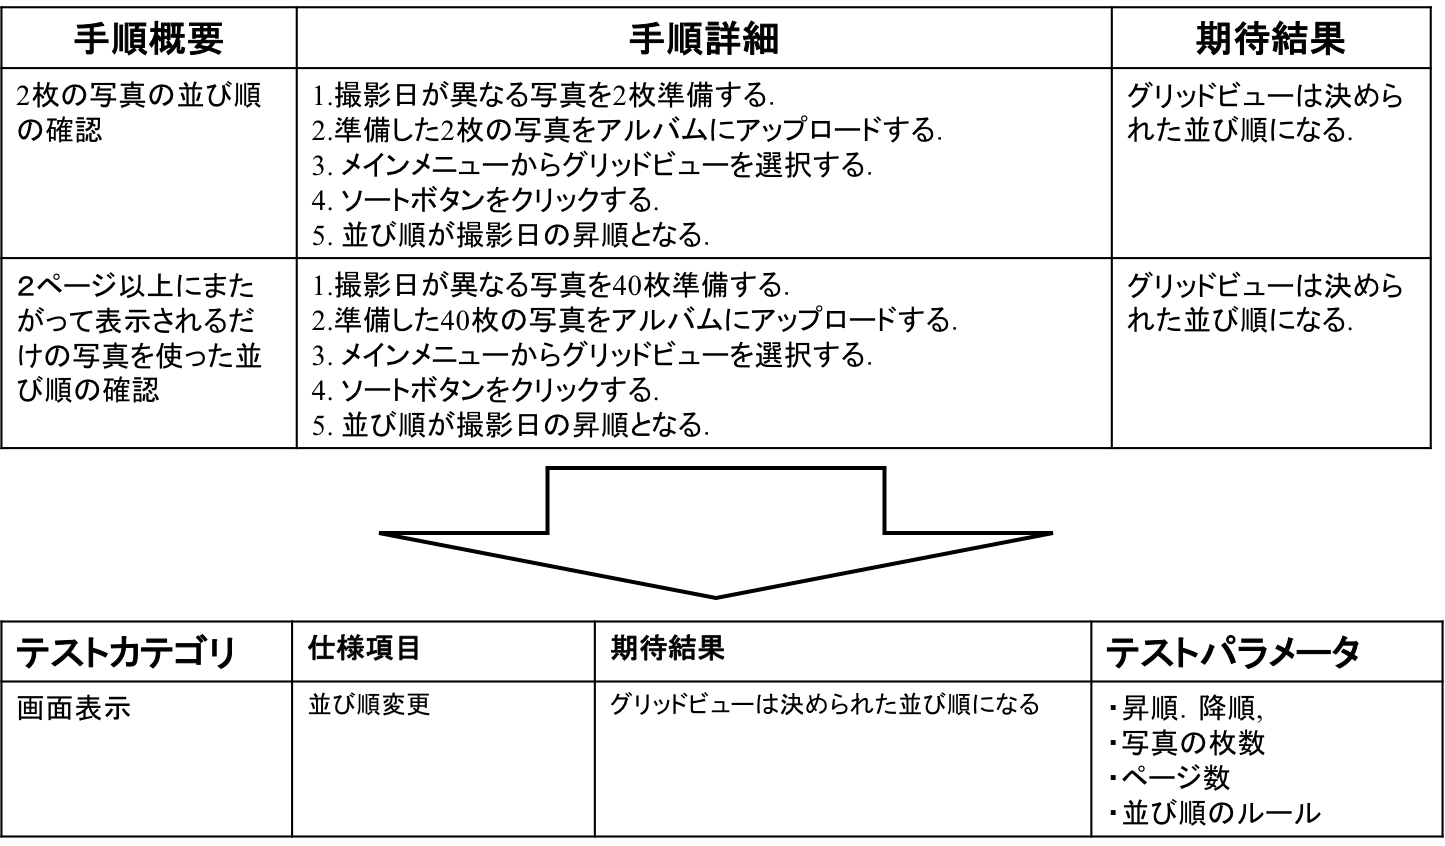
\includegraphics[width=12cm]{./image/D-4-Fig8.png}
\caption{テストケースから仕様項目をまとめる方法の説明}
\label{fig:D-4-Fig8}
\end{center}
\end{figure}

現場で作られたテストケースの数は,アップロードが491ケース,グリッドビューが151ケースであった.
例えば「デバイスからサーバーへ画像ファイルをアップロードして保存が出来ること」という1つの仕様項目に対して,現場で作られたテストケースは,画像の種類(Jpg,Bmpなど),画像のサイズ,アップロードする画像の枚数,画像情報のパターン(ファイル名,撮影日など)といったテストパラメータを組み合わせた複数のテストケースが作られている.
このようなテストケースを整理し,仕様項目として集約していった結果,テスト条件となる仕様項目の数は,アップロードが59項目,グリッドビューが22項目となった.


\item[Step2] 入力データ,出力データの特定

フィーチャセットであるアップロードとグリッドビューのテストベースを分析した結果,以下の4つを入力データ,出力データとして扱うこととした.
\begin{itemize}
 \item 画像データ
 \item 画像の情報
 \item 設定データ
 \item 外部コマンド
\end{itemize}

\item[Step3] I/Oテストデータパターン付与

Step2で特定した入力データと出力データは,Step1で明らかにした仕様項目に対して図~\ref{fig:D-4-Fig8}のように入力データと出力データという列に追記していった.
テスト実行時の追記したデータフローをシミュレーションし,該当するI/Oテストデータパターンを明らかにした.図~\ref{fig:D-4-Fig9}は,ソート順の情報を外部から入力し,内部からの入力となる画像データと一緒になり,外部にソートした画像データを表示している例である.
この場合のI/OテストデータパターンはP7となる.

\begin{figure}[htbp]
\begin{center}
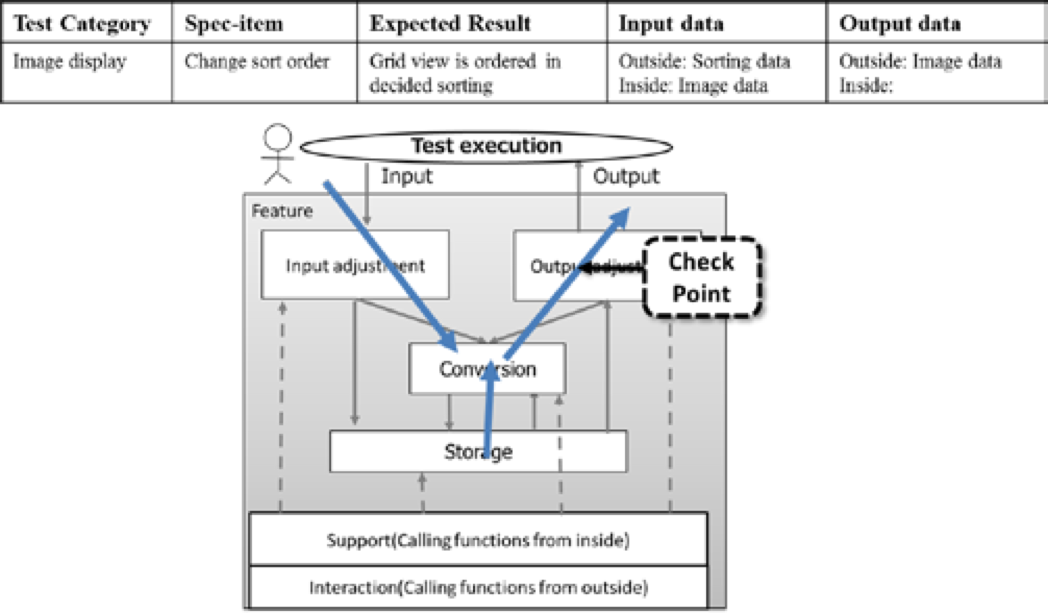
\includegraphics[width=10cm]{./image/D-4-Fig9.png}
\caption{仕様項目に入力データと出力データを加える方法の説明}
\label{fig:D-4-Fig9}
\end{center}
\end{figure}

\end{description}

\subsection{I/Oテストデータパターンを使ったテストベース分析}
I/Oテストデータパターンと既存のテスト分析手法であるテストカテゴリベースドテストを併用してテスト分析を行う.
作業ステップは以下のとおりである:
\begin{itemize}
 \item テストカテゴリを特定する.
 \item テストカテゴリ毎に入力データと出力データを明らかにする.
 \item I/Oテストデータパターンごとのデータフローをシミュレーションしてチェックポイント候補から仕様項目を選択する.
 \item 現場のテストケースを分析した結果をテストカテゴリに分類し,差異を比較する.
\end{itemize}

特定したテストカテゴリは,表~\ref{tab:D-4-TestCategory}のようになった.
サポートと相互作用については,テストカテゴリがトリガーとなる.トリガーから呼び出す$Ta$へのデータフローをシミュレーションして,仕様項目を特定した.


% Table generated by Excel2LaTeX from sheet 'Sheet2'修正
\begin{table}[htbp]
  \centering
  \caption{テストカテゴリ}
    \begin{tabular}{|l|p{5.415em}|l|l|l|l|}
    \hline
          \multicolumn{1}{|p{4em}|}{\textbf{入力調整}} & \textbf{出力調整} & \multicolumn{1}{p{2.5em}|}{\textbf{変換}} & \multicolumn{1}{p{3em}|}{\textbf{貯蔵}} & \multicolumn{1}{p{6em}|}{\textbf{サポート}} & \multicolumn{1}{p{6em}|}{\textbf{相互作用}} \bigstrut\\
    \hline
    \hline
\multicolumn{1}{|l|}{\multirow{3}[2]{*}{画面上操作}} & 画面表示  & \multicolumn{1}{l|}{\multirow{3}[2]{*}{計算}} & \multicolumn{1}{p{4em}|}{設定保存} & 割り込み  & リソース共有 \bigstrut[t]\\
                & メッセージ &       & \multicolumn{1}{p{4em}|}{画像保存} & 中断    & 反映 \\
                & 初期表示  &       &       & データ同時変更 & 並列処理 \bigstrut[b]\\
    \hline
    \end{tabular}%
  \label{tab:D-4-TestCategory}%
\end{table}%

\subsection{IOテストデータパターンの効果検証の結果}
テストカテゴリとI/Oテストデータパターンを使ったテストベースの分析で利用したI/Oテストデータパターンは表~\ref{tab:D-4-IOresult}のようになった.
実験に使ったフィーチャセットであるアップロードとグリッドビューの両方でテストカテゴリとI/Oテストデータパターンを使ったテストベースの分析が適用できた.
そして,両方のフィーチャセットにて,現実の開発で行われたシステムテストレベルのテストケースとI/Oテストデータパターンを使ったテスト分析結果を比較し,現実の開発で使われたテストケースに,テストすべき仕様項目が不足していることが実証できた.
分類に利用したI/Oテストデータパターンは,P5とP8を除く全てであった.

% Table generated by Excel2LaTeX from sheet 'Sheet3'
\begin{table}[htbp]
  \centering
  \caption{I/Oテストデータパターンの出現傾向}
    \begin{tabular}{|p{7em}|p{1.7em}|p{1.7em}|p{1.7em}|p{1.7em}|p{1.7em}|p{1.7em}|p{1.7em}|p{1.7em}|p{1.7em}|}
    \hline
    \multicolumn{1}{|r|}{} & \multicolumn{1}{l|}{P1} & \multicolumn{1}{l|}{P2} & \multicolumn{1}{l|}{P3} & \multicolumn{1}{l|}{P4} & \multicolumn{1}{l|}{P5} & \multicolumn{1}{l|}{P6} & \multicolumn{1}{l|}{P7} & \multicolumn{1}{l|}{P8} & \multicolumn{1}{l|}{P9} \bigstrut\\
    \hline
    アップロード & ○     & ○     & ○     & ○     & X     & ○     & ○     & X     & ○ \bigstrut\\
    \hline
    グリッドビュー & ○     & X     & X     & ○     & X     & X     & ○     & X     & ○ \bigstrut\\
    \hline
    \end{tabular}%
  \label{tab:D-4-IOresult}%
\end{table}%

実プロジェクトのテスト条件との比較をした結果を図~\ref{fig:D-4-Fig10}に示す.
両者を比較すると,I/Oテストデータパターンを利用したテスト分析の結果が実プロジェクトより多くのテスト条件を選択できたことが確認できている.

\begin{figure}[htbp]
\begin{center}
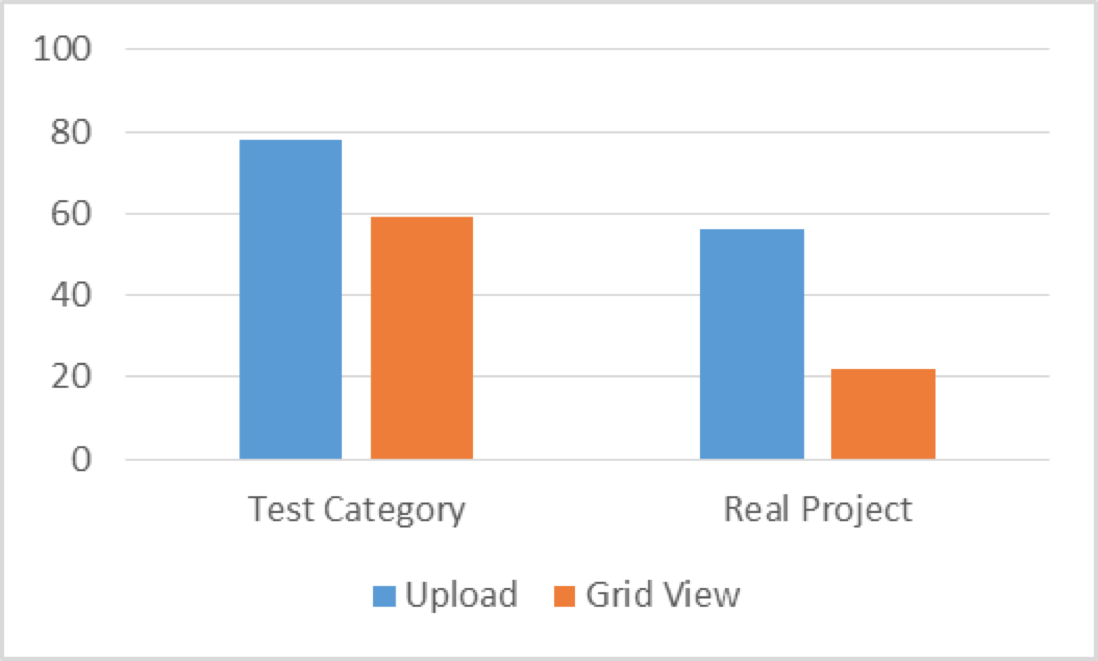
\includegraphics[width=12cm]{./image/D-4-Fig10.png}
\caption{IOテストデータパターンごとの違い}
\label{fig:D-4-Fig10}
\end{center}
\end{figure}

\subsection{I/Oテストデータパターン毎の出現傾向の評価}
現実のプロジェクトで作られたテストケースとI/Oテストデータパターンを使ってテストベースの分析して特定した仕様項目の特定数をP1からP9の分類で出現割合を比較した結果が,表~\ref{tab:D-4-IOtestcompare}である.
% Table generated by Excel2LaTeX from sheet '結果比較'
\begin{table}[htbp]
  \centering
  \caption{I/Oテストデータパターン毎の特定数比較}
    \begin{tabular}{rrrrrrrrr}
    \multicolumn{1}{l}{\textbf{アップロード}} &  &     &       &       &       &       &       &  \bigstrut[b]\\
    \hline
    \multicolumn{1}{|l|}{パターン} &\multicolumn{1}{|l|}{P1} & \multicolumn{1}{l|}{P2} & \multicolumn{1}{l|}{P3} & \multicolumn{1}{l|}{P4} & \multicolumn{1}{l|}{P6} & \multicolumn{1}{l|}{P7} & \multicolumn{1}{l|}{P9} & \multicolumn{1}{l|}{合計} \bigstrut\\
    \hline
    \hline
    \multicolumn{1}{|l|}{TCとI/O} &\multicolumn{1}{|r|}{24} & \multicolumn{1}{r|}{6} & \multicolumn{1}{r|}{12} & \multicolumn{1}{r|}{14} & \multicolumn{1}{r|}{3} & \multicolumn{1}{r|}{7} & \multicolumn{1}{r|}{12} & \multicolumn{1}{r|}{78} \bigstrut\\
    \hline
    \multicolumn{1}{|l|}{現実のPJ} &\multicolumn{1}{|r|}{17} & \multicolumn{1}{r|}{6} & \multicolumn{1}{r|}{10} & \multicolumn{1}{r|}{10} & \multicolumn{1}{r|}{3} & \multicolumn{1}{r|}{5} & \multicolumn{1}{r|}{8} & \multicolumn{1}{r|}{59} \bigstrut\\
    \hline
    &71\%  & 100\% & 83\%  & 71\%  & 100\% & 71\%  & 67\%  & 76\% \bigstrut[t]\\
          &       &       &       &       &       &       &  \\
    \multicolumn{1}{l}{\textbf{グリッドビュー}}  & &       &       &       &       &       &       &  \bigstrut[b]\\
    \hline
    \multicolumn{1}{|l|}{パターン} &\multicolumn{1}{|l|}{P1} & \multicolumn{1}{r|}{--} & \multicolumn{1}{r|}{--} & \multicolumn{1}{l|}{P4} & \multicolumn{1}{r|}{--} & \multicolumn{1}{l|}{P7} & \multicolumn{1}{l|}{P9} & \multicolumn{1}{l|}{合計} \bigstrut\\
    \hline
    \hline
    \multicolumn{1}{|l|}{TCとI/O} &\multicolumn{1}{|r|}{25} & \multicolumn{1}{r|}{--} & \multicolumn{1}{r|}{--} & \multicolumn{1}{r|}{13} & \multicolumn{1}{r|}{--} & \multicolumn{1}{r|}{14} & \multicolumn{1}{r|}{4} & \multicolumn{1}{r|}{56} \bigstrut\\
    \hline
    \multicolumn{1}{|l|}{現実のPJ} &\multicolumn{1}{|r|}{5} & \multicolumn{1}{r|}{--} & \multicolumn{1}{r|}{--} & \multicolumn{1}{r|}{5} & \multicolumn{1}{r|}{--} & \multicolumn{1}{r|}{8} & \multicolumn{1}{r|}{4} & \multicolumn{1}{r|}{22} \bigstrut\\
    \hline
    &20\%  &       &       & 38\%  &       & 57\%  & 100\% & 39\% \bigstrut[t]\\
    \end{tabular}%
  \label{tab:D-4-IOtestcompare}%
\end{table}%

上段のTCとIOは,テストカテゴリとI/Oテストデータパターンを使ってテスト条件を特定した数であり,下段の現実のPJは,現実のプロジェクトでのテスト条件数である.欄外に記載した割合は,上段の数を母数にした場合の下段の現実のプロジェクトのテスト条件数の割合である.
両方の結果を合計したグラフが図~\ref{fig:D-4-Fig11}である.
図~\ref{fig:D-4-Fig11}からは,現実のプロジェクトにて不足していたテスト条件には,I/Oテストデータパターン別にみるとP1が特にテストカテゴリと実プロジェクトの差異が大きいことがわかる.
P1 は外部からの入力を行い,外部に出力する最も単純なパターンであり,I/O テストデータパターンから見ても単純なことを確認するテスト条件が漏れている.

\begin{figure}[htbp]
\begin{center}
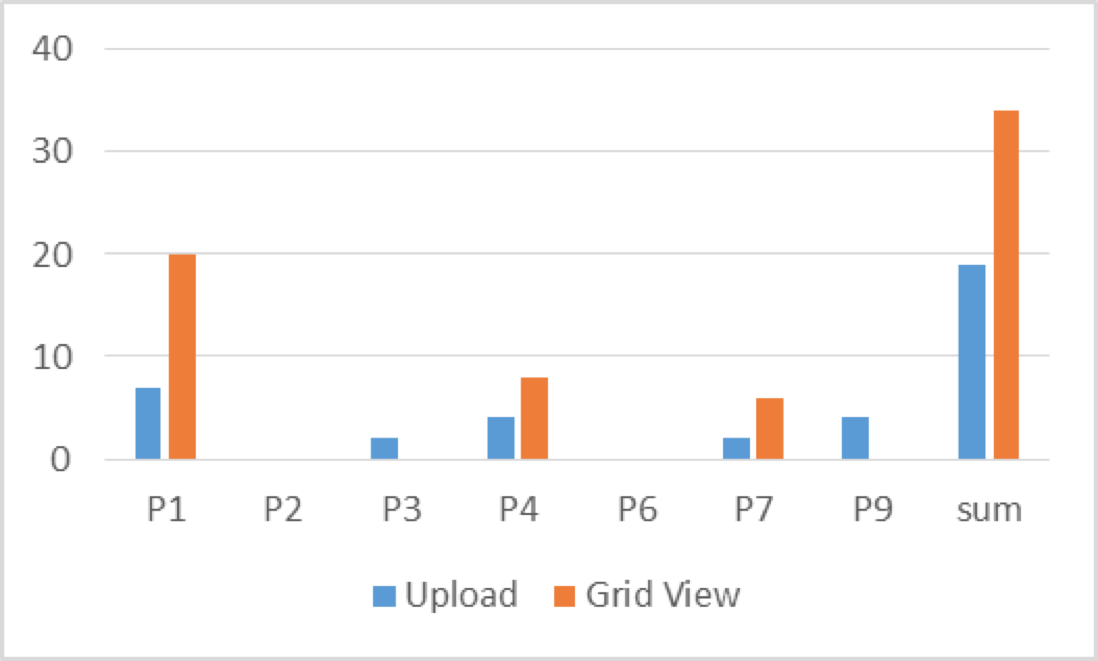
\includegraphics[width=12cm]{./image/D-4-Fig11.png}
\caption{IOテストデータパターンごとの違い}
\label{fig:D-4-Fig11}
\end{center}
\end{figure}

\subsection{I/Oテストデータパターンにて特定したテスト条件}
表~\ref{tab:D-4-ER-1}から表~\ref{tab:D-4-ER-4}に,I/Oテストデータパターンにて新たに特定したテスト条件となる仕様項目を全て列挙した.
これらのテスト条件は,全て今回のデータのI/Oのシミュレーションを行い網羅的にテストベースを確認することで特定できたものである.
I/Oテストデータパターンにて新たに特定したテスト条件には,論理的機能構造の要素別に見ると入力調整, 出力調整に分類できるテスト条件,例えばメッセージが現れることや入力制御といった単純な仕様項目でも漏れていることが確認できる.

一般的に,テスト条件となる仕様項目の一覧を作成せずに具体的なインスタンスとなるテストケースを列挙していく場合,テストパラメータ組合せの数量の多さに合わせてテストケースの数量が膨大になるため,網羅すべきテスト条件仕様項目の見易さが低下するため,仕様項目の数が不足することが多い.
実験結果も同様の傾向となった.

また,現実のプロジェクトで作られたテストケースからまとめ直したテスト条件の一覧を表~\ref{tab:D-4-ER2-1}から表~\ref{tab:D-4-ER2-6}に列挙した.
これらのテスト条件はI/Oテストデータパターンを使ったシミュレーションでも全て特定可能であった.
% Table generated by Excel2LaTeX from sheet 'Sheet2'
\begin{table}[htbp]
  \scriptsize
  \centering
  \caption{I/Oテストデータパターンにて特定したテスト条件(1/4)}
    \begin{tabular}{|p{8em}|p{7em}|p{9em}|p{9em}|p{3em}|p{12em}|}
\cline{1-6}   フィーチャセット & テストカテゴリ  & 仕様項目 & 期待結果  & I/O   & 入出力データ \bigstrut\\
    \hline
    アップロード & データ同時変更 & アップロード中のアップロード済み画像のアルバム移動 & ロックがかかりできないこと & P9    & 外入:画像 内入:移動元画像
外出:件数 内出:画像 \bigstrut\\
    \hline
    アップロード & データ同時変更 & アップロード中のアップロード済み画像の情報変更 & ロックがかかりできないこと & P9    & 外入:情報 内入:画像情報
外出:変情 内出:画像情報 \bigstrut\\
    \hline
    アップロード & データ同時変更 & アップロード中のアップロード先アルバム名変更 & ロックがかかりできないこと & P9    & 外入:画像,アルバム名 内入:元アルバム名
外出:件数 内出:画像 \bigstrut\\
    \hline
    アップロード & データ同時変更 & アップロード中のアップロード前画像のアルバム移動 & ロックがかかりできないこと & P9    & 外入:画像 内入:移動元画像
外出:件数 内出:画像 \bigstrut\\
    \hline
    アップロード & メッセージ & 「画像を選択」時の選択枚数表示 & 「○枚の画像を選択中」というメッセージが出るか & P1    & 外入:画像選択 内入:--
外出:メッセージ 内出:-- \bigstrut\\
    \hline
    アップロード & メッセージ & 重複画像だけでアップロードした際の画像のアップロード & 「アップロードできない」というメッセージがでるか? & P1    & 外入:画像選択 内入:--
外出:メッセージ 内出:-- \bigstrut\\
    \hline
    アップロード & メッセージ & 「画像を選択」画面初期表示 & 「画像を選択」と表記が出ること & P1    & 外入:文字 内入:--
外出:文字 内出:-- \bigstrut\\
    \hline
    アップロード & メッセージ & 「画像を選択」時の選択枚数表示にて,選択済みの画像を押下 & 「○枚の画像を選択」というメッセージの枚数が減ること & P1    & 外入:画像選択 内入:--
外出:メッセージ 内出:-- \bigstrut\\
    \hline
    アップロード & メッセージ & 「画像を選択」時の選択枚数表示にて,選択済みの画像を押下 & 選択数が0になった場合,「画像を選択」と表記が出ること & P1    & 外入:画像選択 内入:--
外出:メッセージ 内出:-- \bigstrut\\
    \hline
    アップロード & 画像表示  & \multicolumn{1}{p{7.5em}|}{「アルバムに追加」でのアルバム一覧} & アルバム一覧の表示順が正しいこと & P4    & 外入:-- 内入:画像サムネイル,アルバム名
外出:画像サムネイル,アルバム名 内出:-- \bigstrut\\
    \hline
    アップロード & 画像表示  & \multicolumn{1}{p{7.5em}|}{「画像を選択」時の画像表示順} & 撮影日昇順で表示されること & p4    & 外入:-- 内入:画像
外出:画像 内出:-- \bigstrut\\
    \hline
    アップロード & 初期表示  & \multicolumn{1}{p{7.5em}|}{「アップロード」画面の操作} & 新規アルバムYYYY/MM/DDというアルバム名が表示されること & P4    & 外入:-- 内入:初期設定
外出:アルバム名 内出:-- \bigstrut\\
    \hline
    アップロード & 初期表示  & \multicolumn{1}{p{7.5em}|}{「アップロード」画面の操作} & 「すでにアップロード済みの画像を保存しない」がONになっていること & P4    & 外入:-- 内入:初期設定
外出:設定 内出:-- \bigstrut\\
    \hline
    アップロード & 画面上操作 & \multicolumn{1}{p{7.5em}|}{「アップロード」画面の操作} & 「すでにアップロード済みの画像を保存しない」がON→OFF→ONに変更できること & P1    & 外入:設定入力 内入:--
外出:設定 内出:-- \bigstrut\\
    \hline
    \end{tabular}%
  \label{tab:D-4-ER-1}%
\end{table}%

% Table generated by Excel2LaTeX from sheet 'Sheet4'
\begin{table}[htbp]

  \scriptsize
  \centering
  \caption{I/Oテストデータパターンにて特定したテスト条件(2/4)}
  \begin{tabular}{|p{8em}|p{7em}|p{9em}|p{9em}|p{3em}|p{12em}|}
\cline{1-6}   フィーチャセット & テストカテゴリ  & 仕様項目 & 期待結果  & I/O   & 入出力データ \bigstrut\\
    \hline
    アップロード & 画面上操作 & \multicolumn{1}{p{7.5em}|}{「アルバムに追加」に表示されるアルバム名} & 「全画像」を選択できること & P7    & 外入:操作入力 内入:登録済画像
外出:登録済画像 内出:-- \bigstrut\\
    \hline
    アップロード & 画面上操作 & 「画像を選択」での画像選択 & 画像にタップするとチェックがつくこと & P7    & 外入:選択 内入:画像
外出:チェックアイコン 内出:-- \bigstrut\\
    \hline
    アップロード & 中断    & \multicolumn{1}{p{7.5em}|}{ネットワーク切断から再開したときのアップロード} & 一定以上の時間が過ぎるとアップロードが再開しない(要確認) & P1    & 外入:画像 内入:--
外出: メッセージ 内出:-- \bigstrut\\
    \hline
    アップロード & 画像保存  & \multicolumn{1}{p{7.5em}|}{アルバムの枚数が200枚以上になる枚数で画像を選択してアップロードのエラーが出た後に別のアルバムを選択してアップロード} & アップロードできた画像がNISにて表示できること & P3    & 外入:画像 内入:--
外出:枚数 内出:画像 \bigstrut\\
    \hline
    アップロード & 画像保存 & \multicolumn{1}{p{7.5em}|}{アップロードした画像の画質} & アップロードした画像が崩れていないこと & P3    & 外入:画像 内入:--
外出:枚数 内出:画像 \bigstrut\\
    \hline
    グリッドビュー & メッセージ & 選択画面初期表示 & 「画像を選択」と表記が出ること & P1    & 入力:文字
出力:文字 \bigstrut\\
    \hline
    グリッドビュー & メッセージ & 選択解除ボタン押下 & 「画像を選択」と表記が出ること & P1    & 入力:選択 文字
出力:文字 \bigstrut\\
    \hline
    グリッドビュー & メッセージ & \multicolumn{1}{p{7.5em}|}{選択済みの画像を押下} & 「○枚の画像を選択」というメッセージの枚数が減ること & P1    & 入力:選択
出力:文字 \bigstrut\\
    \hline
    グリッドビュー & メッセージ & \multicolumn{1}{p{7.5em}|}{選択済みの画像を押下} & 選択数が0になった場合,「画像を選択」と表記が出ること & P1    & 入力:選択
出力:文字 \bigstrut\\
    \hline
    グリッドビュー & メッセージ & 全て選択ボタン押下 & 「アルバムを選択中」というメッセージが出ること & P1    & 入力:選択
出力:文字 \bigstrut\\
    \hline
    グリッドビュー & メッセージ & 未選択の画像を押下 & 「○枚の画像を選択」というメッセージが出ること & P1    & 入力:選択
出力:文字 \bigstrut\\
    \hline
    グリッドビュー & 画像表示  & 1画面あたりの表示ファイル数 & 縦:4×10.横:3×7になること & P4    & 入力:既存設定
出力:文字 画像 \bigstrut\\
    \hline
    \end{tabular}%
  \label{tab:D-4-ER-2}%
\end{table}%

% Table generated by Excel2LaTeX from sheet 'Sheet4'
\begin{table}[htbp]
  \scriptsize
  \centering
  \caption{I/Oテストデータパターンにて特定したテスト条件(3/4)}
  \begin{tabular}{|p{8em}|p{7em}|p{9em}|p{9em}|p{3em}|p{12em}|}
\cline{1-6}   フィーチャセット & テストカテゴリ  & 仕様項目 & 期待結果  & I/O   & 入出力データ \bigstrut\\
    \hline
    グリッドビュー & 画像表示  & スクロール時の枚数表示 & 複数ページのスクロールでファイルの日付と,現在の枚数順/全体の枚数が画面中央に表示されること & p7    & 入力:スクロール
出力:文字 画像 \bigstrut\\
    \hline
    グリッドビュー & 画像表示  & 画像ファイルの並び順 & 左から右方向に埋まっていくこと。 & P4    & 入力:既存設定
出力:文字 画像 \bigstrut\\
    \hline
    グリッドビュー & 画像表示  & 画像ファイルの並び順 & 2行目になるとまた左から埋まること & P4    & 入力:既存設定
出力:文字 画像 \bigstrut\\
    \hline
    グリッドビュー & 画像表示  & 更新ボタン押下 & 別デバイスで新しい画像の追加,名称の変更などをしていた場合,変更した画像に更新されること & P4    & 入力:既存設定
出力:画像 \bigstrut\\
    \hline
    グリッドビュー & 共有    & 他ビューの並び順影響有無 & 他のアルバムやビューで設定した並び順の影響を受けないこと & p4    & 入力:既存設定
出力:画像 \bigstrut\\
    \hline
    グリッドビュー & 設定保存  & 画面の並び順設定用画面 & 前回選択した並び順にチェックがついていること & p7    & 入力:並び順
出力:並び順 \bigstrut\\
    \hline
    グリッドビュー & 設定保存  & 画面の並び順設定用画面 & デフォルトでチェックされていること & p7    & 入力:並び順
出力:並び順 \bigstrut\\
    \hline
    グリッドビュー & 画面上操作 & OKボタン押下 & 全画像,カテゴリから移動したグリッドビューの場合のみOKボタンが現れ,共有設定画面に遷移する & P1    & 入力:既存設定
出力:画像 \bigstrut\\
    \hline
    グリッドビュー & 画面上操作 & \multicolumn{1}{p{7.5em}|}{アルバム追加ボタン押下} & アルバムから移動したグリッドビューの場合,アルバム追加画面に遷移する & P1    & 入力:既存設定
出力:文字 画像 \bigstrut\\
    \hline
    グリッドビュー & 画面上操作 & ダウンロードボタン押下 & アルバムから移動したグリッドビューの場合,DLサイズ選択画面に遷移する & P1    & 入力:既存設定
出力:文字 \bigstrut\\
    \hline
    グリッドビュー & 画面上操作 & 削除ボタン押下 & アルバムから移動したグリッドビューの場合,削除画面に遷移 & P1    & 入力:既存設定
出力:文字 \bigstrut\\
    \hline
    \multicolumn{1}{|l|}{グリッドビュー} & 画面上操作 & 選択画面初期表示 & 全画像から遷移したグリッドビューの場合,選択,解除,削除,アルバム追加,DLボタン出ない.OKボタン出る. & P1    & 入力:既存設定
出力:文字 画像 \bigstrut\\
    \hline
    \multicolumn{1}{|l|}{グリッドビュー} & 画面上操作 & 選択画面初期表示 & カテゴリから遷移したグリッドビューの場合,全画像からの遷移と同じであり,かつカテゴリを選択する選択用ビューがグレーアウトする & P1    & 入力:既存設定
出力:文字 画像 \bigstrut\\
    \hline
    \end{tabular}%
  \label{tab:D-4-ER-3}%
\end{table}%

% Table generated by Excel2LaTeX from sheet 'Sheet4'
    \begin{table}[htbp]
      \scriptsize
      \centering
      \caption{I/Oテストデータパターンにて特定したテスト条件(4/4)}
      \begin{tabular}{|p{8em}|p{7em}|p{9em}|p{9em}|p{3em}|p{12em}|}
    \cline{1-6}   フィーチャセット & テストカテゴリ  & 仕様項目 & 期待結果  & I/O   & 入出力データ \bigstrut\\
        \hline
    \multicolumn{1}{|l|}{グリッドビュー} & 画面上操作 & 選択画面初期表示 & 端末の写真のグリッドビューの場合,最初から選択画面となり,チェックをすることでOKボタンが有効になる & P1    & 入力:既存設定
出力:文字 画像 \bigstrut\\
    \hline
    \multicolumn{1}{|l|}{グリッドビュー} & 画面上操作 & 選択解除ボタン押下 & 画面上の全ての画像のチェックが外れること & p1    & 入力:選択
出力:アイコン \bigstrut\\
    \hline
    \multicolumn{1}{|l|}{グリッドビュー} & 画面上操作 & \multicolumn{1}{p{7.5em}|}{選択済みの画像を押下} & 画像のチェックが外れること & p1    & 入力:選択
出力:アイコン \bigstrut\\
    \hline
    \multicolumn{1}{|l|}{グリッドビュー} & 画面上操作 & 全て選択ボタン押下 & 画面上の全ての画像にチェックがつくこと & p1    & 入力:選択
出力:アイコン \bigstrut\\
    \hline
    \multicolumn{1}{|l|}{グリッドビュー} & 画面上操作 & 未選択の画像を押下 & 画像のチェックがつくこと & p1    & 入力:選択
出力:アイコン \bigstrut\\
    \hline
    \multicolumn{1}{|l|}{グリッドビュー} & 画面上操作 & 未選択の画像を押下 & 全てチェックの場合,押下した画像以外のチェックが全て外れること & p1    & 入力:選択
出力:アイコン \bigstrut\\
    \hline
    \multicolumn{1}{|l|}{グリッドビュー} & 画面上操作 & フロービューボタン押下 & フロービューに遷移すること & P7    & 入力:既存設定
出力:文字 画像 \bigstrut\\
    \hline
    \multicolumn{1}{|l|}{グリッドビュー} & 画面上操作 & マップビュー押下 & マップビューに遷移すること & P7    & 入力:既存設定
出力:文字 画像 \bigstrut\\
    \hline
    \multicolumn{1}{|l|}{グリッドビュー} & 画面上操作 & 画像選択ボタン押下 & ピクチャービューに遷移すること & P7    & 入力:既存設定
出力:文字 画像 \bigstrut\\
    \hline
    \multicolumn{1}{|l|}{グリッドビュー} & 画面上操作 & 画面の並び順設定用画面 & ファイル名,アップロード名,撮影日,ファイルサイズ,ファイル形式,お気に入り,マイルールの順で一覧表示されていること & P1    & 入力:既存設定
出力:文字 \bigstrut\\
    \hline
    \multicolumn{1}{|l|}{グリッドビュー} & 画面上操作 & 並び順の変更 & 一覧項目の横をタップするとチェックがつくこと & p1    & 入力:設定
出力:設定 \bigstrut\\
    \hline
    グリッドビュー & 中断    & ネットワーク切断時のグリッドビュー初期表示 & キャッシュがある場合,キャッシュされた画像が一覧表示されること & P4    & 入力:既存設定
出力:文字 画像 \bigstrut\\
    \hline
    グリッドビュー & 中断    & ネットワーク切断時のグリッドビュー初期表示 & キャッシュの限界を超えた場合,その画像が一覧表示されないこと & P4    & 入力:既存設定
出力:文字 画像 \bigstrut\\
    \hline
    グリッドビュー & 中断    & ネットワーク切断時の更新ボタン押下 & キャッシュがある場合,更新ボタンを押すと別デバイスの変更が反映されず画像が表示される & P4    & 入力:既存設定
出力:文字 画像 \bigstrut\\
    \hline
    \end{tabular}%
    \label{tab:D-4-ER-4}%
  \end{table}%


  \begin{table}[htbp]
    \scriptsize
    \centering
    \caption{開発プロジェクトにてテストで使われたテスト条件(1/6)}
    \begin{tabular}{|p{8em}|p{7em}|p{9em}|p{9em}|p{3em}|p{12em}|}
  \cline{1-6}   フィーチャセット & テストカテゴリ  & 仕様項目 & 期待結果  & I/O   & 入出力データ \bigstrut\\
      \hline
      \hline
    アップロード & データ同時変更 & アップロード先のアルバムに複数のデバイスからアップロードして結果的に合計が200枚以上になる枚数で画像を選択してアップロード & (要確認) & P3    & 外入:画像 内入:---
外出:件数 内出:画像 \bigstrut\\
    \hline
    アップロード & データ同時変更 & アップロード中のアップロード済み画像が入るアルバム削除 & 未整理の画像としてアップロードされる?(要確認) & P9    & 外入:画像 内入:元アルバム名
外出:件数 内出:画像 \bigstrut\\
    \hline
    アップロード & データ同時変更 & アップロード中のアップロード済み画像の削除 & (要確認) & P9    & 外入:画像 内入:削除元画像
外出:件数 内出:画像 \bigstrut\\
    \hline
    アップロード & データ同時変更 & アップロード中のアップロード前画像の削除 & (要確認) & P9    & 外入:画像 内入:削除元画像
外出:件数 内出:画像 \bigstrut\\
    \hline
    アップロード & データ同時変更 & アップロード中のアップロード前画像の情報変更 & (要確認) & P9    & 外入:情報 内入:画像情報
外出:変情 内出:画像情報 \bigstrut\\
    \hline
    アップロード & メッセージ & 100枚以上の画像を選択してアップロード & 「規定以上の枚数はアップロードできない」というメッセージが出て処理が終了する & P3    & 外入:画像選択,画像 内入:--
外出:件数 内出:画像 \bigstrut\\
    \hline
    アップロード & メッセージ & アップロード先のアルバムの枚数が200枚以上になる枚数で画像を選択してアップロード & 「規定以上の枚数はアップロードできない」というメッセージ出てが出て処理が終了する & P1    & 外入:画像選択 内入:--
外出:メッセージ 内出:-- \bigstrut\\
    \hline
    アップロード & メッセージ & マイフォト全体での枚数のMAXを超えたときの画像のアップロード & 画像が上限に達したことを知らせるメッセージが出て処理が終了する & P1    & 外入:画像選択 内入:--
外出:メッセージ 内出:-- \bigstrut\\
    \hline
    アップロード & メッセージ & アルバム数がMAX(3500)を超えたときの新規アルバム追加のアップロード & アルバムが上限に達したことを知らせるメッセージが出て処理が終了する & P1    & 外入:画像選択 内入:--
外出:メッセージ 内出:-- \bigstrut\\
    \hline
    アップロード & メッセージ & アップロード終了時のDL/UL一覧へのメッセージ & DL/UL一覧で終了したことがわかること & P1    & 外入:画像 内入:--
外出:メッセージ 内出:-- \bigstrut\\
    \hline
    アップロード & 画像表示  & アップロードした画像の表示確認 & 画像にアップロードアイコンが付与されて表示されている & p4    & 外入:-- 内入:画像
外出:画像 内出:-- \bigstrut\\
    \hline
    アップロード & 画像表示  & 「アルバムに追加」でのアルバム一覧 & アルバムが無い場合はアルバムが出てこないこと & P4    & 外入:-- 内入:画像サムネイル,アルバム名
外出:画像サムネイル,アルバム名 内出:-- \bigstrut\\
    \hline
    アップロード & 画像表示  & 「画像を選択」で表示される画像種類 & 動画(アップロードできないコンテンツ)が選択画面に出てこないこと & P4    & 外入:-- 内入:画像
外出:画像 内出:-- \bigstrut\\
    \hline
    アップロード & 画像表示  & 「画像を選択」時の画像表示 & 複数ページにまたがる場合はスクロールできること & p7    & 外入:フリック 内入:画像
外出:画像 内出:-- \bigstrut\\
    \hline
    \end{tabular}%
  \label{tab:D-4-ER2-1}%
\end{table}%


\begin{table}[htbp]
  \scriptsize
  \centering
  \caption{開発プロジェクトにてテストで使われたテスト条件(2/6)}
  \begin{tabular}{|p{8em}|p{7em}|p{9em}|p{9em}|p{3em}|p{12em}|}
\cline{1-6}   フィーチャセット & テストカテゴリ  & 仕様項目 & 期待結果  & I/O   & 入出力データ \bigstrut\\
    \hline
    \hline
    アップロード & 画像表示  & \multicolumn{1}{p{8em}|}{アップロード状況確認画面} & アップロードできた画像が先に表示されこれからアップロードする画像が色が黒っぽく表示されること & P9    & 外入:画像 内入:登録済画像
外出:画像登録結果 内出:画像 \bigstrut\\
    \hline
    アップロード & 画像表示  & \multicolumn{1}{p{8em}|}{アップロード状況確認画面} & ドラッグ&ドロップでアップロード済とアップロード前の画像の表示を入れ替えることができないこと & P7    & 外入:操作入力 内入:画像
外出:表示位置 内出:-- \bigstrut\\
    \hline
    アップロード & 画像表示  & \multicolumn{1}{p{8em}|}{アップロード状況確認画面} & 複数ページにまたがる場合はスクロールできること & p7    & 外入:フリック 内入:画像
外出:画像 内出:-- \bigstrut\\
    \hline
    アップロード & 画像保存  & \multicolumn{1}{p{8em}|}{画像のアップロード実施} & アップロードできた画像がNISにて表示できること & P2    & 外入:画像 内入:--
外出:-- 内出:画像 \bigstrut\\
    \hline
    アップロード & 画像保存  & \multicolumn{1}{p{8em}|}{画像のアップロード実施} & JPGとして保存されること & P2    & 外入:画像 内入:--
外出:-- 内出:画像 \bigstrut\\
    \hline
    アップロード & 画像保存  & \multicolumn{1}{p{8em}|}{重複画像のアップロード無効} & 重複画像がアップロードされていないこと & P2    & 外入:画像(なし) 内入:--
外出:-- 内出:画像(なし) \bigstrut\\
    \hline
    アップロード & 画像保存  & \multicolumn{1}{p{8em}|}{アップロード画像の名称がMAXを超える} & 要確認??? & P2    & 外入:画像(なし) 内入:--
外出:-- 内出:画像(なし) \bigstrut\\
    \hline
    アップロード & 割り込み  & \multicolumn{1}{p{8em}|}{アップロード中に電話などの割り込み入る} & 処理は継続する(要確認) & P3    & 割り込みで処理をバックグランドにするタスクだが,I/Oとしてはその間P3が続いている
外入:画像 内入:--
外出:枚数 内出:画像 \bigstrut\\
    \hline
    アップロード & 計算    & \multicolumn{1}{p{8em}|}{アップロード中のDL/UL一覧} & DL/UL一覧で何枚までアップロードしているかがわかること & P3    & 外入:画像 内入:--
外出:枚数 内出:画像 \bigstrut\\
    \hline
    アップロード & 画面上操作 & \multicolumn{1}{p{8em}|}{「アルバム名編集」でのアルバム名が空白} & アルバム名の保存ボタンが押下ができないこと & P1    & 外入:設定入力 内入:--
外出:設定 内出:-- \bigstrut\\
    \hline
    アップロード & 画面上操作 & \multicolumn{1}{p{8em}|}{「アルバム名編集」でのアルバム名が空白} & 40文字を超えて入力できないこと & P1    & 外入:設定入力 内入:--
外出:設定 内出:-- \bigstrut\\
    \hline
    アップロード & 画面上操作 & \multicolumn{1}{p{8em}|}{「アルバムに追加」でのアルバム名変更} & 新規アルバム名変更でアルバム名が変更できること & P1    & 外入:アルバム名入力 内入:--
外出:アルバム名 内出:-- \bigstrut\\
    \hline
    アップロード & 画面上操作 & \multicolumn{1}{p{8em}|}{「アルバムに追加」に表示されるアルバム名} & 既存のアルバムを選択できること & P1    & 外入:-- 内入:アルバム名
外出:アルバム名 内出:-- \bigstrut\\
    \hline
    アップロード & 画面上操作 & 「画像を選択」での画像選択 & ドラッグによる表示順移動ができないこと & P7    & 外入:操作入力 内入:画像
外出:表示位置 内出:-- \bigstrut\\
    \hline
    アップロード & 画面上操作 & 「画像を選択」でのアップロードボタン押下 & DL/ULアイコンが表示されもとの画面にもどること & P3    & 外入:選択,画像 内入:--
外出:枚数 内出:画像 \bigstrut\\
    \hline
    \end{tabular}%
  \label{tab:D-4-ER2-2}%
\end{table}%

\begin{table}[htbp]
  \scriptsize
  \centering
  \caption{開発プロジェクトにてテストで使われたテスト条件(3/6)}
  \begin{tabular}{|p{8em}|p{7em}|p{9em}|p{9em}|p{3em}|p{12em}|}
\cline{1-6}   フィーチャセット & テストカテゴリ  & 仕様項目 & 期待結果  & I/O   & 入出力データ \bigstrut\\
    \hline
    \hline
    アップロード & 画面上操作 & \multicolumn{1}{l|}{「画像を選択」でのアップロードボタン押下} & 画像が選択されていないときにはアップロード画面へ遷移しないこと & P1    & 外入:選択 内入:--
外出: メッセージ 内出:-- \bigstrut\\
    \hline
    アップロード & 画面上操作 & DL/UL一覧のXボタン押下 & キャンセルダイアログに遷移すること & P1    & 外入:選択 内入:---
外出: メッセージ 内出:--- \bigstrut\\
    \hline
    アップロード & 画面上操作 & DL/UL一覧の件数 & DL/UL一覧が20件を超えると古いものから削除されること & P1    & 外入:選択 内入:--
外出: メッセージ 内出:-- \bigstrut\\
    \hline
    アップロード & 画面上操作 & DL/UL中に新規にアップロードを行う & Waiting状態になり,前の処理が終了するとアップロードを開始すること & P3    & 外入:選択 画像 内入:--
外出: メッセージ 内出:画像 \bigstrut\\
    \hline
    アップロード & 画面上操作 & DL/ULアイコンからの遷移 & DL/UL一覧へ遷移すること & P3    & 外入:選択 画像 内入:--
外出: 登録済み件数 内出:画像 \bigstrut\\
    \hline
    アップロード & 画面上操作 & DL/UL一覧でUL中を選択 & 状況確認画面へ遷移する & P9    & 外入:選択 画像 内入:登録済画像情報
外出: 登録済み件数 内出:画像 \bigstrut\\
    \hline
    アップロード & 画面上操作 & DL/UL一覧でのクローズボタン押下 & DL/ULアイコンに戻る。遷移先画面は遷移元画面と同じであること。 & P3    & 外入:選択 画像 内入:--
外出: アイコン 内出:画像 \bigstrut\\
    \hline
    アップロード & 画面上操作 & キャンセル実行 & DL/UL一覧にてキャンセルボタンが出てこなくなること。 & P1    & 外入:選択 内入:--
外出: 表示 内出:-- \bigstrut\\
    \hline
    アップロード & 中断    & アップロードのネットワーク切断 & アップロードが止まる(要確認) & P1    & 外入:止めるための情報 画像 内入:--
外出: メッセージ 内出:-- \bigstrut\\
    \hline
    アップロード & 中断    & ネットワーク切断から再開したときのアップロード & 中断していたアップロードが再開すること。 & P3    & 外入:画像 内入:--
外出: 件数 内出:画像 \bigstrut\\
    \hline
    アップロード & 中断    & アップロード中にアプリからログアウトした際のアップロード & アップロードを継続するか?(要確認) & P2    & 外入:画像 内入:--
外出: ーー 内出:画像 \bigstrut\\
    \hline
    アップロード & 中断    & キャンセル時のアップロード画像の扱い & キャンセルするまでの画像がアップロードできて,その後の画像はアップロードしていないこと & P1    & 外入:選択 内入:--
外出: 表示 内出:-- \bigstrut\\
    \hline
    アップロード & 中断    & アップロード中にアプリからログアウトした際のDL/UL一覧 & DL/UL一覧が全てクリアされる & P1    & 外入:選択 内入:--
外出: 表示 内出:-- \bigstrut\\
    \hline
    アップロード & 中断    & アップロード中にアプリを終了した際のDL/UL一覧 & DL/UL一覧が全てクリアされる & P1    & 外入:選択 内入:--
外出: 表示 内出:-- \bigstrut\\
    \hline
    アップロード & 中断    & アップロード中にアプリを終了した際のアップロード & 中断する(要確認) & P1    & 外入:選択 内入:--
外出: 表示 内出:-- \bigstrut\\
    \hline
    アップロード & 中断    & アップロード中にデバイスの電源を切った際のDL/UL一覧 & DL/UL一覧が全てクリアされる & P1    & 外入:選択 内入:--
外出: 表示 内出:-- \bigstrut\\
    \hline
    \end{tabular}%
  \label{tab:D-4-ER2-3}%
\end{table}%


\begin{table}[htbp]
  \scriptsize
  \centering
  \caption{開発プロジェクトにてテストで使われたテスト条件(4/6)}
  \begin{tabular}{|p{8em}|p{7em}|p{9em}|p{9em}|p{3em}|p{12em}|}
\cline{1-6}   フィーチャセット & テストカテゴリ  & 仕様項目 & 期待結果  & I/O   & 入出力データ \bigstrut\\
    \hline
    \hline
    アップロード & 反映    & アップロードした画像の詳細情報 & 位置情報など全部の情報が登録されていること & P4    & 外入:-- 内入:画像
外出: 画像 内出:-- \bigstrut\\
    \hline
    アップロード & 反映    & アップロードした画像の場所 & 指定したアルバムの中にだけ表示されていること & P4    & 外入:-- 内入:画像
外出: 画像 内出:-- \bigstrut\\
    \hline
    アップロード & 反映    & アップロードした画像の表示 & 各種ビューでバリエーションとして確認 & P4    & 外入:-- 内入:画像
外出: 画像 内出:-- \bigstrut\\
    \hline
    アップロード & 反映    & アップロード中画像のダウンロード & ダウンロードができること & P4    & 外入:-- 内入:画像
外出: 画像,枚数 内出:-- \bigstrut\\
    \hline
    アップロード & 反映    & アップロードした際に作成したアルバム確認 & マイフォトにてアルバムが出来ていること & P4    & 外入:-- 内入:アルバム
外出: アルバム,枚数 内出:-- \bigstrut\\
    \hline
    アップロード & 並列処理  & アップロード中に共有フォルダを作成する & 影響を与えないでアップロードが続く & P3    & 割り込みで処理をバックグランドにするタスクだが,I/Oとしてはその間P3が続いている
外入:画像 内入:--
外出:枚数 内出:画像 \bigstrut\\
    \hline
    アップロード & 並列処理  & アップロード中に設定画面へ遷移し操作する & 設定をしている間もアップロードが続くこと & P3    & 割り込みで処理をバックグランドにするタスクだが,I/Oとしてはその間P3が続いている
外入:画像 内入:--
外出:枚数 内出:画像 \bigstrut\\
    \hline
    アップロード & 並列処理  & アップロード中に他のビューで閲覧する & 各種ビューでバリエーションとして確認 & P7    & 割り込みで処理をバックグランドにするタスクだが,I/Oとしてはその間P3が続いている
外入:選択 内入:画像
外出:画像 内出:-- \bigstrut\\
    \hline
    アップロード & 並列処理  & アップロード中に他のビューで閲覧する & 閲覧中もアップロードが続く & P3    & 割り込みで処理をバックグランドにするタスクだが,I/Oとしてはその間P3が続いている
外入:画像 内入:--
外出:枚数 内出:画像 \bigstrut\\
    \hline
    アップロード & データ同時変更 & アップロード中のアップロード済み画像が入るアルバム削除 & アルバムを削除した後に同じアルバム名を作って再度アップロードを繰り返した際にアップロードができること & P9    & 外入:画像 内入:削除元画像
外出:件数 内出:画像 \bigstrut\\
    \hline
    アップロード & 画像保存  & アルバムの枚数が200枚以上になる枚数で画像を選択してアップロードのエラーが出た後に別のアルバムを選択してアップロード & アップロードした画像の詳細情報の登録ができていること & P2    & 入力:画像情報
出力:画像情報 \bigstrut\\
    \hline
    アップロード & 画像保存  & 一度アップロードした画像を削除してまた同じ画像をアップロードする & アップロードできた画像がNISにて表示できること & P3    & 外入:画像 内入:--
外出:枚数 内出:画像 \bigstrut\\
    \hline
    \end{tabular}%
  \label{tab:D-4-ER2-4}%
\end{table}%



\begin{table}[htbp]
  \scriptsize
  \centering
  \caption{開発プロジェクトにてテストで使われたテスト条件(5/6)}
  \begin{tabular}{|p{8em}|p{7em}|p{9em}|p{9em}|p{3em}|p{12em}|}
\cline{1-6}   フィーチャセット & テストカテゴリ  & 仕様項目 & 期待結果  & I/O   & 入出力データ \bigstrut\\
    \hline
    \hline
    アップロード & 画面上操作 & \multicolumn{1}{p{8em}|}{DL/UL中にダウンロードが失敗やキャンセルなど処理が中断した後に新規にアップロードを行う} & 直前のパターンが失敗する,キャンセルする,失敗が続く,エラーがでるといった状況を複数組み合わせてアップロード対象がアップロードできることを確認する & P3    & 外入:画像 内入:--
外出:枚数 内出:画像 \bigstrut\\
    \hline
    アップロード & 反映    & \multicolumn{1}{p{8em}|}{アップロード中画像がエラーになる場合のダウンロード} & エラーなったときのその直前の成功した画像,アップロードが失敗する画像のダウンロードができること & P4    & 外入:-- 内入:画像
外出: 画像,枚数 内出:-- \bigstrut\\
    \hline
    グリッドビュー & メッセージ & \multicolumn{1}{p{8em}|}{規定枚数以上の画像を押下} & 「一度に選択できる画像は100枚までです」というメッセージが出る & P1    & 入力:選択
出力:文字 \bigstrut\\
    \hline
    グリッドビュー & 画像表示  & デフォルトの画像ファイル表示順 & デフォルト設定にあわせて表示されること & P4    & 入力:既存設定
出力:文字 画像 \bigstrut\\
    \hline
    グリッドビュー & 画像表示  & デフォルトの画像レイアウト & 縦横が基の画像のとおりに表示されること & P4    & 入力:既存設定
出力:文字 画像 \bigstrut\\
    \hline
    グリッドビュー & 画像表示  & 画像枚数がゼロ & 空白で表示されること & P1    & 入力:既存設定
出力:文字 \bigstrut\\
    \hline
    グリッドビュー & 画像表示  & 並び順設定後の画像ファイル表示順 & ファイル名で表示されること(昇順,降順) & p7    & 入力:並び順
出力:文字 画像 \bigstrut\\
    \hline
    グリッドビュー & 画像表示  & 並び順設定後の画像ファイル表示順 & アップロード名の昇順で表示されること & p7    & 入力:並び順
出力:文字 画像 \bigstrut\\
    \hline
    グリッドビュー & 画像表示  & 並び順設定後の画像ファイル表示順 & 撮影日の昇順で表示されること & p7    & 入力:並び順
出力:文字 画像 \bigstrut\\
    \hline
    グリッドビュー & 画像表示  & 並び順設定後の画像ファイル表示順 & ファイルサイズの昇順で表示されること & p7    & 入力:並び順
出力:文字 画像 \bigstrut\\
    \hline
    グリッドビュー & 画像表示  & 並び順設定後の画像ファイル表示順 & ファイル形式の昇順で表示されること & p7    & 入力:並び順
出力:文字 画像 \bigstrut\\
    \hline
    グリッドビュー & 画像表示  & 並び順設定後の画像ファイル表示順 & お気に入りの昇順で表示されること & p7    & 入力:並び順
出力:文字 画像 \bigstrut\\
    \hline
    グリッドビュー & 画像表示  & 並び順設定後の画像ファイル表示順 & マイルールで設定した順番で表示されること & p7    & 入力:並び順
出力:文字 画像 \bigstrut\\
    \hline
    グリッドビュー & 画像表示  & 戻るボタン押下 & マイフォト画面に遷移すること & P4    & 入力:既存設定
出力:画像 \bigstrut\\
    \hline
    グリッドビュー & 設定保存  & ドラッグドロップによるマイルール作成 & ドラッグドロップの表示位置変更結果をマイルールとして保存すること & p9    & 入力:画像,並び順
出力:画像,マイルール \bigstrut\\
    \hline
    グリッドビュー & 画面上操作 & 選択画面初期表示 & 全て選択ボタン,選択解除ボタンの位置が上もしくは下のどちらかに現れること & P1    & 入力:既存設定
出力:文字 \bigstrut\\
    \hline
    グリッドビュー & 画面上操作 & 「並び順」ボタン押下 & 画像の並び順画面に遷移すること & p1    & 入力:既存設定
出力:並び順 \bigstrut\\
    \hline
    \end{tabular}%
  \label{tab:D-4-ER2-5}%
\end{table}%


\begin{table}[htbp]
  \scriptsize
  \centering
  \caption{開発プロジェクトにてテストで使われたテスト条件(6/6)}
  \begin{tabular}{|p{8em}|p{7em}|p{9em}|p{9em}|p{3em}|p{12em}|}
\cline{1-6}   フィーチャセット & テストカテゴリ  & 仕様項目 & 期待結果  & I/O   & 入出力データ \bigstrut\\
    \hline
    \hline
    \multicolumn{1}{|c|}{グリッドビュー} & 画面上操作 & スクロール & 上下にスクロールできること & p1    & 入力:選択
出力:表示 \bigstrut\\
    \hline
    \multicolumn{1}{|c|}{グリッドビュー} & 画面上操作 & ドラッグドロップによる表示位置変更 & ドラッグドロップした位置に移動できること & p9    & 入力:画像,並び順
出力:画像,マイルール \bigstrut\\
    \hline
    \multicolumn{1}{|c|}{グリッドビュー} & 画面上操作 & 画像押下  & ピクチャービューに遷移すること & P7    & 入力:既存設定
出力:文字 画像 \bigstrut\\
    \hline
    \multicolumn{1}{|c|}{グリッドビュー} & 画面上操作 & 並び順の変更 & 変更したい並び順を選択するとグリッドビュー画面に遷移すること & p9    & 入力:画像,並び順
出力:画像,並び順 \bigstrut\\
    \hline
    \multicolumn{1}{|c|}{グリッドビュー} & 画面上操作 & 並び順の変更 & 変更したソート順で表示されること & p9    & 入力:画像,並び順
出力:画像,並び順 \bigstrut\\
    \hline
    グリッドビュー & 中断    & ネットワーク切断時のグリッドビュー初期表示 & キャッシュがない場合,グリッドビューを表示すると画像が表示されないこと & P4    & 入力:既存設定
出力:画像(なし) \bigstrut\\
    \hline
    グリッドビュー & 中断    & ネットワーク切断時の更新ボタン押下 & キャッシュがない場合,更新ボタンを押すと「インターネット接続がオフラインのようです」のメッセージがでる & P4    & 入力:既存設定
出力:画像(なし) \bigstrut\\
    \hline
    \end{tabular}%
  \label{tab:D-4-ER2-6}%
\end{table}%



\newpage
\section{まとめ}
本章では,テスト実行時のデータ入出力の要素で分類し網羅的に分析するI/Oテストデータパターンを提案した.そして,入手した現実の開発プロジェクトのテストケースを使い,I/Oテストデータパターンで特定したテスト条件との比較を試みた.
提案したI/Oテストデータパターンで特定したテスト条件と実プロジェクトで作られるテストケースと比較して,不足しているテスト条件の発見が可能であることが確認できた.

%%%%%%%%%%%%%%%%%%%%%%%
%%%%%%%%%%%%%%%%%%%%%%%
\chapter{データ共有タスク間の順序組合せテストケース抽出手法} \label{chap:5}
本章では,統合テストにおける状態遷移間の組合せに着目する,
実践の場においては,S1網羅基準に膨大なテスト工数を要する課題があることから,その対処として経験的なノウハウを基に重要なテストケースを抽出する方法が用いられている\cite{yumoto2006}.
そのひとつの方法として,状態遷移のS1網羅基準のうち,重要な順序組合せを見つけ出す実践的なナレッジとして,状態はタスク内で保持するデータとして実装されることに着目したテストケースの抽出方法がある.
この方法は,保持するデータに対する操作順序が影響することから,データに対するタスクの操作順序パターンを使い,状態遷移の組合せをタスクの順序組合せとしてテストする.
順序組合せのテストは,ソフトウェアに変更を加えた場合の変更波及のテストケースとして有効になる.

\newpage
\section{研究の概要} \label{sec:5-1}
\subsection{研究の目的} \label{sec:5-1-1}
前章では,I/O テストデータパターンで単一の$Ta$に対するデータの入出力からテスト条件を網羅的に特定する方法を提案した.
本章では,単一の$Ta$に対するデータの入出力による副作用を確認するテストに着目する.
これは論理的機能構造でのサポートと相互作用に分類されるテスト条件となる.
これらのテスト条件を特定する際のトリガーの一つとして,他処理への反映がある.
他処理への反映をテスト条件に加える目的は,$AS$の一部に変更を加えた場合のその波及の確認が必要となるためである.

ソフトウェアの一部に変更を加えた場合,その変更の波及を探る変更波及解析(Change Impact Analysis)は,実務上の大きな課題である.
産業界において変更にかかる活動は,新規開発よりも大きな割合を占めている.
ゼロから新規にソフトウェアを開発するケースは稀であり,何らかの流用を基に変更を加える開発が主流となっている.
開発方法においてもアジャイルが主流となり,変更の積み重ねによって開発が行われている.
しかし,変更波及を合理的に制御する技術は,ソフトウェア工学とって未完成の分野である\cite{arnold1996software}.
変更の背景は,時代と共に課題を難しくしている.
ソフトウェアの多様化と複雑化,再利用範囲の増大などから変更波及の範囲が拡大し,かつ安易な変更による弊害など課題が山積している.
これらの課題に対してソフトウェア工学は十分な解を提供できていない状況にある\cite{li2013survey}.
本章では,状態遷移を持つソフトウェアにおいて,変更波及がデータベースや外部変数などの保持データを介して生ずる場合のテストについて考える.
課題の一つは,網羅基準である.データフローテストの全使用法(AU法)\cite{beiz90}を基にして,変更波及のテスト網羅基準を波及全使用法(Impact Data All Used:IDAU)として提案する.
もう一つの課題は,IDAU法を満たす具体的な変更波及のテストケースの抽出方法である.変更波及のテストの設計手法として,順序組合せテストを提案する.
最後に,ここで提案するIDAU法のコストの評価,すなわちテストケースの数を従来技法である状態遷移テストのS1網羅基準と比較をして考察を行い,提案する方法が合理的であることを示す.


\newpage
\section{変更波及とその解析}
本節では,提案する網羅基準やテスト設計手法の前提となる,システムの構成と変更について定義し,変更波及をテストする課題について詳細を示す.

\subsection{変更と変更波及}
$AS$に対して,何らかの変更を加える場合について考える.
変更には,なんらかの意図があり,$AS$が持つ機能の変更であったり,不具合に対する変更や,性能や保守性の改善のためのリファクタリングであったりする.
本論文では,変更の意図については取り扱わず,$AS$の構成要素(タスク,状態,保持データ)に対する具体的な変更について考える.ただし,テスト実行するためには,タスクを動かすことが必要となる.そのため,以降の議論はタスクに焦点を絞る.%1-1対応

ひとつの変更$Q$について考える.
変更$Q$は,タスク群$Ta$のあるタスク$Ta_i$に対して行われたとする.
変更$Q$は,コードの削除や追加を含み,その結果$Ta_i$の版$R$が$R+1$に変更される.
この変更の結果を$Ta^{R}_i$から$Ta^{R+1}_i$とする.

変更$Q$の波及には,3つのケースが考えられる.
\begin{enumerate}
  \item 変更波及が無い場合.(リファクタリングに相当)
  \item 変更波及が他のタスクへ波及しない場合.%3-7対応
  \item 変更波及が他のタスクへ波及する場合.
\end{enumerate}

3.の変更波及は,タスク間の参照が図\ref{fig:fig-2}に示すように状態と保持データに限られるならば,該当する状態や保持データの参照を介した範囲が限られると考えられる.
本論文では,この考え方から波及を受けるタスクを特定し,その合理的なテスト設計について論じる.


%−−−-図2を入れる

\begin{figure}[b]
\begin{center}
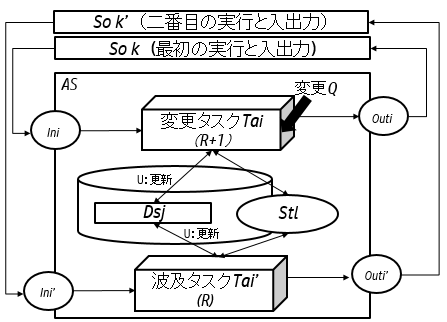
\includegraphics[scale=0.5]{./image/fig-2.png}
\end{center}
\caption{変更タスクと変更波及}
\label{fig:fig-2}
\end{figure}

変更波及,あるいはその解析(Change Impact Analysis)に関する研究は古くから行われている.プロダクトラインやUML図面群を基に依存関係生成モデルを用いて波及解析を行う研究がある\cite{gomaa2005designing}\cite{2008kotani}\cite{briand2003impact}
タスク内のデータフローを基に変更波及を詳細に解析した研究がある\cite{campbell1990}.
データベースなど保有データを基に変更波及解析を行う研究も行われている\cite{maule2008impact}\cite{2011ogawa}.
一方,状態と状態遷移はマルコフ過程として実装されているので,過去の状態が未来の状態に影響しない.状態遷移に関する波及解析の研究は見当たらないのはそのためだと推測する.%3-8対応
\cite{LSOF}
\cite{kang1990feature}
\subsection{状態と変更波及のテスト}
変更波及は,保持データを介して波及タスクへ伝達する.状態や状態遷移自身は変更波及に関与しないが,変更波及のテストにおいて与えるデータの順序において状態を考慮する必要が生じる.

保持データの構成について考える.その要素を$Ds=\{Ds_1,Ds_2,\cdots,Ds_j,\cdots,Ds_d\}$とし,変更波及を受ける保持データの要素を$Ds_j$とする.
保持データに対する操作は,データのライフサイクルである「生成:C」「参照:R」「更新:U」「削除:D」を記したCRUD図で定義する.
$Ds_j$を介して変更波及が生ずるのは,変更タスク$Ta_i$において「生成:C」あるいは「更新:U」が行われ,他のタスクで「参照:R」が行われた場合に波及タスクとなる.

保持データのライフサイクル上の「生成:C」「参照:R」「更新:U」「削除:D」などの操作は,無条件に行われるのではなく,操作するタスクの制御フローに沿って行われる.
制御フローは,2階層として捉えることができる.上位の制御フローはタスクの実行順序により決定される大きな制御の流れに相当する.
個々のタスク内の制御フローが下位にあたる.個々のデータ参照実行文はその制御フロー上の条件文で実行が決定される.
条件にはタスクへの入力,保持データ,状態が含まれる.

変更波及を確認するには,変更が波及した保持データを参照するデータフローに沿ってテストを設計することになる.
このデータフローを決定するのは,関係するタスクの実行順序とタスク内の制御フローであり,その制御フローを決定する際に状態が影響する.
状態による制御が想定通りに行われない欠陥は,タスクの実行順序により決定される大きな制御の流れの判断のための状態の確認を,タスク実行のあるタイミングでのみ行っていることが原因となる.%1-2対応による追記
よって,実際のテスト実行においては状態を考慮する必要が生ずる.

\subsection{変更波及テストの網羅基準}

テストにおける網羅基準については,その強度を含め制御フローとデータフローの観点から研究が行われ体系が作られている\cite{beiz90}.
最も弱い網羅基準は制御フローのみに着目した実行文網羅,次が分岐網羅であり,最も強い網羅基準はデータフローを含めた全パス網羅(All Paths)である.%3-9
全パステストは,すべての分岐の積であり現実的には実現不可能のため,全使用法(All Uses)が推奨されている\cite{beiz90}.

変更波及をテストする場合,波及に関与するデータに着目し,そのデータフローテストを行う.
一般的な全使用法は「データを定義したすべての場所から始まり,データを使用するすべての場所に至るまでのパスセグメントを最低限1つを含むテストケース」と定義されている\cite{beiz90}.
この定義を変更タスクと波及タスクとの関係に置き換え「変更タスクにおいてデータの生成および更新があるデータを使用するすべてのタスク(波及タスク)を2つのタスクを実行するまでに経由するルートにかかわらず最低限1つ含むテストケース」とし,波及全使用法とする.

\newpage
\section{順序組合せによるテストケース抽出法} \label{sec:5-2}
本節では,状態遷移テスト設計におけるS1 網羅基準ではテストケース数が爆発するが,S0網羅基準では漏れが生じるという課題を解決する手法として順序組合せテストを提案する.

\subsection{入力情報}
 一般的にテストケース抽出のために必要な入力情報をテストベースと呼ぶ\cite{Demarco}.
提案手法に必要なテストベースは DFD,ER 図,CRUD 図である.以下,DFD,ER 図,CRUD 図を簡潔に説明する.

\begin{itemize}

\item DFD(データフローダイアグラム)

DFDはシステムにおけるデータの流れを表現した有向グラフであり,要求分析において用いられている.
DFDはデータ指向設計の要として用いられ,オブジェクト指向設計においても抽象化する前段階として実践の場で用いられている.

DFDは,最上位のコンテキストレベルから階層として詳細化され,各階層は1枚以上のDFDから成る\cite{Demarco}.
テストベースとして用いる場合,テストの範囲はDFDで与えられるとする.DFDの階層が下がると単体テストとなり,上がると統合テストとなる.

DFDはノードとエッジからなる.
ノードは3種類の要素である$N$個のタスク(プロセス)$Ta$と,$M$個の保持データ(データストア)$Ds$と,$L$個の源泉(外部エンティティ)$So$から構成されている.%3-11対応
3種類の要素を一意に特定する際は$Ta_i$,$Ds_j$,$So_k$と表記する.

エッジは,ノードからノードへのつながりを有向線分で表記している.エッジはデータの流れを表しており,制御の流れは表していない.
エッジの特定は,起点ノードと終点ノードを用いて行う.
ある特定のタスクからデータストアへの入力がある場合のエッジの特定は,$Ta_i/Ds_j$となり,源泉から出力してタスクで処理をする場合は,$So_k/Ta_i$と表す.%3-12対応

\item ER図

ER図はシステムにおけるエンティティ間の関係を示す図であり,UMLのクラス図に対応している.
DFDでは表現できないエンティティの詳細化やエンティティ間の関係について示しており,DFDと共に用いられている.

ここでは,DFDのデータストア$Ds_j$が持つエンティティと,CRUD図の対応から,後述する拡張CRUD図を作成するために用いる.
よって,テストベースとしては,システムすべてのER図を必要とするものではない.

\item CRUD図

CRUD図とは,タスク$Ta_i$からデータストア$Ds_j$への$C$:生成,$U$:更新,$R$:参照,$Ds$:削除の操作を表した図である\cite{Politano}.
CRUD図から,DFDとER図では表現されていないタスクのエンティティへの操作を知ることができる.

本論文では,タスクがデータストアに対して行う操作を特定するためにCRUD図を用いる.
タスク$Ta_i$のデータストア$Ds_j$に対する操作が$U$:更新であればタスクによる操作はエッジを介した操作として$Ta_i/Ds_jU$と表記する.
ただし,タスクが操作するデータストアが1つだけの場合は,$Ta_iU$といった省略した表記を使う.
\end{itemize}

\subsection{順序組合せテストの概要} \label{sec:5-2-1}
提案する手法は,2タスク間の順序組合せを対象とする.
2タスク間の順序組合せの抽出は以下のルールを適用する.
\begin{itemize}

\item ルール1:変更タスクの特定
%20170305
%対象とするDFDにおけるタスクにおいて,源泉$So$からの入力エッジがあり,かつデータストア$Ds$へ出力エッジを持つタスクを選択し順序組合せの変更タスク群$P\{Ta\}$とする.

対象とするDFD内の変更タスクのうち,データストア$Ds$へ出力エッジを持つタスクを選択し,順序組合せの変更タスク群$P\{Ta\}$とする.%3-14対応
変更タスク群からの出力するデータストア群を$P\{Ds\}$とする.

\item ルール2:波及タスクの特定

ルール1で求めた$P\{Ds\}$からの入力エッジを持つタスクを波及タスク群$S\{Ta\}$として特定する.

\item ルール3:順序組合せテストケースの抽出

拡張CRUD図を基に変更タスク群$P\{Ta\}$とそのデータストア群$P\{Ds\}$を介する波及タスク群$S\{Ta\}$を組合せ,順序組合せのテストケースとする.
\end{itemize}

以降からは,順序組合せを抽出してテストケースとするまでの実施手順を詳細に説明する.

\subsection{ルール1:変更タスクの特定}
% Table generated by Excel2LaTeX from sheet 'Sheet1'
\begin{table}[t]
\caption{拡張CRUD図}
\label{CRUDIO}
\begin{center}
\begin{tabular}{r|r|r|r|r|r|r}
\multicolumn{1}{c|}{タスク} & \multicolumn{3}{c|}{データストア} & \multicolumn{3}{c}{源泉} \\
\cline{2-7}\multicolumn{1}{c|}{} & $Ds_1$ & $...$ & $Ds_j$ & $So_1$ & $...$ & $So_k$ \\
\hline
\hline
$Ta_1$ &   &   &   &   &   &  \\
\hline
$...$ &   &   &   &   &   &  \\
\hline
$Ta_i$ &   &   &   &   &   &  \\
    \hline
\end{tabular}%
%\halflineskip
\end{center}
\end{table}

ルール1を用いて変更タスクとそのデータストアを特定し,拡張CRUD図の変更タスク部分を作成する.


拡張CRUD図とは,テストベースとして与えられたDFD,ER図,CRUD図から$P\{Ta\}$の各$Ta_i$と関連する$So_k$,そして$P\{Ds\}$となる$Ds_j$の関係を追加して作成したものである.
表 ~\ref{CRUDIO}に拡張CRUD図の表記を示す.
拡張CRUD図のデータストアに対する情報は$C$,$U$,$R$,$D$のいづれか,または組合せか空白である.
源泉に対する情報は$In$か$Out$,または組合せか空白である.
空白は関係が無いことを示す.

\begin{enumerate}
\item 源泉からの入力エッジを持つ変更タスクの特定

%状態について記載するように変更した.補集合で表現するようにした
%元のストーリーである、外部入力があるタスクはそのままにして、更に抽出する要素として、「変更のある」を追加した.
テストケースは,外部からのテスト対象への入力から,外部への出力結果を確認するものであるため,テスト入力とテスト結果のペアで構成されている.
そこで,テスト対象範囲の外からの入力,即ち$So_k$からの入力エッジを持つ$Ta_i$を見つける必要がある.
この特性を持ったタスクのうち,さらに変更のあるタスク群を変更タスクの集合となる$P\{Ta\}$候補とする.
変更が特定の状態でのみ起こり得る場合は,タスクの後に変更が起きる状態を[$St_l$]と記載する.
%上記は追加部分

\item データストアへの出力エッジを持つタスク特定

$Ta_i$から$Ds_j$への出力エッジは,$C$か$U$か$D$の操作を行うことを意味する.CRUD図から該当する出力エッジを持つ$Ta_i$を選択する.
$P\{Ts\}$候補の中から,該当する$Ta_i$を選び,変更タスク群$P\{Ta\}$を確定する.

\item 中間の拡張CRUD図作成

拡張CRUD図には,変更タスク群$P\{Ta\}$に該当する$So_k$から$Ta_i$への入力($In$),もしくは$Ta_i$から$So_k$への出力($Out$)の情報を付加する.
特定した$Ta_i$に対して,入力となる$So_k$に$In$を記入し,$Ds_j$についてはCRUD図を参照して$C$か$U$か$D$かその組合せかを記入する.
中間の拡張CRUD図として例示した表 ~\ref{CRUDIO2}では,3つの源泉$\{So_1,So_2,So_3\}$と3つのデータストア$\{Ds_1,Ds_2,Ds_3\}$があり,2つのタスク$\{Ta_1[St_1],Ta_3[St_1]\}$が変更タスクである.
この段階で作成する拡張CRUD図は,作業途中のものである.

\end{enumerate}


% Table generated by Excel2LaTeX from sheet 'Sheet1'
\begin{table}[t]
  \centering
  \caption{中間の拡張CRUD図の例}
    \begin{tabular}{r|r|r|r|r|r|r}
    \multicolumn{1}{c|}{タスク} & \multicolumn{3}{c|}{データストア} & \multicolumn{3}{c}{源泉} \\
\cline{2-7}    \multicolumn{1}{c|}{} & $Ds_1$ & $Ds_2$ & $Ds_3$ & $So_1$ & $So_2$ & $So_3$ \\
    \hline
    \hline
    $Ta_1[St_1]$ & $CU$ &   &   & $In$ &   &  \\
    \hline
    $Ta_3[St_1]$ &   & $C$ &   & $In$ &   &  \\
    \hline
    \end{tabular}%
 \label{CRUDIO2}
\end{table}%



\subsection{ルール2:波及タスクの特定}
ルール2を用いて波及タスク群を特定し,拡張CRUD図へ波及タスク部分を追加し図を完成させる.

\begin{enumerate}
\item データストアを介した波及タスク特定
%\item データストアを介した\end{enumerate}波及タスク特定
%なぜ\UTF{2613}と−がテストしなくてよいかということを追記した.
先に作成した中間の拡張図から変更タスクの操作が$C$か$U$か$D$であるデータストアに着目する.
着目したデータストアに対してエッジを持つタスクが波及タスクの候補となる.
波及タスクとして選択するタスクは表 ~\ref{table:3}に示す表の○印の組合せに該当するタスクである.
\begin{table}[h]
\caption{タスク間のデータ共有の組合せパターン}
\label{table:3}
\begin{center}
\begin{tabular}{c|c||c|c|c|c}
\hline
\multicolumn{2}{c||}{}& \multicolumn{4}{c}{$P\{Ta\}$}\\
\multicolumn{2}{c||}{}& C & R & U& D\\
\hline\hline
$S\{Ta\}$&C&×&×&×&◯\\
\cline{2-6}
&R&◯&-&◯& -\\
\cline{2-6}
&U&◯&-&◯&×\\
\cline{2-6}
&D&◯&- &◯&×\\
\hline
\end{tabular}
%\halflineskip
\end{center}
\end{table}
波及タスクは, C:生成,U:更新,D:削除を選択する.
”-”をつけた組合せは,データストアを介した影響が生じないため,組合せテストの対象としない.
”×”をつけた組合せは仕様上有り得ない組合せであり,ありえないことの確認は,順序組合せを網羅しなくともよいため,組合せテストの対象としない.

着目したデータストアに対してエッジを持つタスクが波及タスクのうち,源泉に出力エッジを持つタスクを波及タスクとして特定する.
特定した波及タスクを拡張CRUD図に追記し完成させる.
\item 拡張CRUD図の完成
波及タスク候補のうち,源泉に出力エッジを持つタスクを波及タスクとして特定する.
波及タスクの特性をDFDより読み取り,特定する.
特定した波及タスクを拡張CRUD図に追記し完成させる.
完成させた拡張CRUD図の例を表~\ref{excrud}に示す.
この例では,
データストア$Ds_1$から源泉$So_2$への流れをタスク$Ta_2[St_1]$が行い,
データストア$Ds_2$から源泉$So_3$への流れをタスク$Ta_5[St_1]$が行っていることを示している.
\end{enumerate}
% Table generated by Excel2LaTeX from sheet 'Sheet1'
\begin{table}[t]
  \centering
  \caption{完成した拡張CRUD図の例}
    \begin{tabular}{r|r|r|r|r|r|r}
    \multicolumn{1}{c|}{タスク} & \multicolumn{3}{c|}{データストア} & \multicolumn{3}{c}{源泉} \\
\cline{2-7}    \multicolumn{1}{c|}{} & $Ds_1$ & $Ds_2$ & $Ds_3$ & $So_1$ & $So_2$ & $So_3$ \\
    \hline
    \hline
    $Ta_1[St_1]$ & $CU$ &   &   & $In$ &   &  \\
    \hline
    $Ta_3[St_1]$ &   & $C$ &   & $In$ &   &  \\
    \hline
    $Ta_2[St_1]$ & $R$ &   &   &   & $Out$ &  \\
    \hline
    $Ta_5[St_1]$ &   & $R$U &   &   &   & $Out$ \\
    \end{tabular}%
  \label{excrud}%
\end{table}%

\subsection{ルール3:順序組合せテストケースの抽出}
\begin{enumerate}
\item 変更タスクと波及タスクの組合せを抽出

拡張CRUD図から変更タスクを選ぶ.
先に作成した拡張CRUD図の例(表~\ref{excrud}を参照)であれば,$Ta_1[St_1],Ta_3[St_1]$である.
次に変更タスクが操作しているデータストアと,それを操作している波及タスクを対応付ける.
例では,$Ta_1[St_1]  \xrightarrow[Ds_1]{} Ta_2[St_1]$と$Ta_3[St_1]  \xrightarrow[Ds_2]{}  Ta_5[St_1]$である.
\item データストアに対する操作の組合せ

操作の組合せとは変更タスクと波及タスクの操作の組合せである.
%表 ~\ref{excrud}の例であれば,変更タスクのデータストアに対する操作,$Ta_1$は$Ds_1$に対して$CU$の操作を行っている.%3-21対応
表 ~\ref{excrud}の例であれば,変更タスクのデータストアに対する操作である$Ta_1$は,$Ds_1$に対して$C$と$U$の操作を行っている.
波及タスク$Ta_2$の操作は$R$である.
組合せは$C  \rightarrow R$と$U  \rightarrow R$となる.
変更タスクと波及タスク間に介在するデータストアが1つであれば$\xrightarrow[Ds_1]{}$を省略して$\rightarrow$で表してもよい.
また変更の発生条件となる状態が1つであれは,$[St_1]$を省略してもよい.
表~\ref{excrud}の例における全組合せは,$Ta_1C \rightarrow Ta_2R$,$Ta_1U \rightarrow Ta_2R$,$Ta_3C \rightarrow Ta_2R$,$Ta_3C \rightarrow Ta_2U$の4個である.

\item テストケース表の完成

変更タスクと波及タスクの操作の組合せをテストケースとしてまとめる.表 ~\ref{TCLISTSAMPLE}にその例を示す.概要の部分は,当該組合せが持つ入力の条件や出力の特性を仕様から抜き出して記載する.
\end{enumerate}

% Table generated by Excel2LaTeX from sheet 'Sheet1'
\begin{table}[t]
  \centering
  \caption{順序組合せテストによる論理的テストケースの例}
    \begin{tabular}{l|l|l}
    No & 論理的テストケース & 順序組合せ \\
    \hline
    1 & 概要 & $Ta_1C \rightarrow Ta_2R$ \\
    \hline
    2 & 概要 & $Ta_1U \rightarrow Ta_2R$ \\
    \hline
    3 & 概要 & $Ta_3C \rightarrow Ta_2R$ \\
    \hline
    4 & 概要 & $Ta_3C \rightarrow Ta_2U$ \\
    \hline
    \end{tabular}%
\label{TCLISTSAMPLE}
\end{table}%

以上の手順で,順序組合せテストに必要なテストケースを抽出する.
ここで用いたテストケースとは,ISTQBの定義による論理的テストケースに相当する\cite{ISTQB}.

具体的な値や期待結果,該当の処理までの状態を遷移させていく手順まで定義した記述を具体的テストケースと呼ぶが,本論文では扱わない.

\newpage
\section{評価実験} \label{sec:5-3}
\subsection{実験の概要} \label{sec:5-3-1}

本節では,旅行代理店向けフライト予約システムの仕様を用いて,3章で述べた実施手順を適用し,順序組合せが抽出できることを確認する.

\subsection{題材の概要}
フライト予約システムの概要を以下に示す.
%・フライト予約システムの概要を説明する\\
\begin{figure}[h]% fig.1
\setbox0\vbox{%
{\small
%{\footnotesize
\hbox{\verb/<フライト予約システム概要>/}
\hbox{\verb/・旅行代理店用に開発したフライト予約サーバにインターネット経由で/}
\hbox{\verb/ アクセスできる専用のクライアントアプリケーション./}
\hbox{\verb/・旅行代理店の窓口での利用を想定しており,ユーザ認証されたユーザ/}
\hbox{\verb/ のみ利用可能である./}
\hbox{\verb/・旅行代理店の窓口数(クライアント数)は50としており,同時に予約/}
\hbox{\verb/ 処理を行うことができる./}
\hbox{\verb/・旅行代理店にて取り扱う全ての航空会社の飛行機の予約が可能で/}
\hbox{\verb/ ある./}
\hbox{\verb/・本システムは,フライト予約サーバを仲介して複数の航空会社のシス/}
\hbox{\verb/ テムと同期をする./}
\hbox{\verb/・チケット情報や残チケット数は同期することで最新に更新される./}
\hbox{\verb/・フライトの新規予約、予約内容の更新,削除が可能である.更新と/}
\hbox{\verb/ 削除は新規予約したユーザのみ可能である./}
\hbox{\verb/・以下はシステム範囲外/}
\hbox{\verb/ -チケット代金の決済(別システムと連携して行うため)./}
\hbox{\verb/ -マスタ情報設定(他システムとの共用マスタ設定アプリケーションが/}
\hbox{\verb/  あるため)./}
}
}
\begin{center}
\fbox{\box0}
\end{center}
\caption{フライト予約システムの概要}
\label{OVSPEC}
\end{figure}

\begin{figure*}[tb] %ER図とDFD.最初と最後に*を入れると1段で入る
\begin{center}
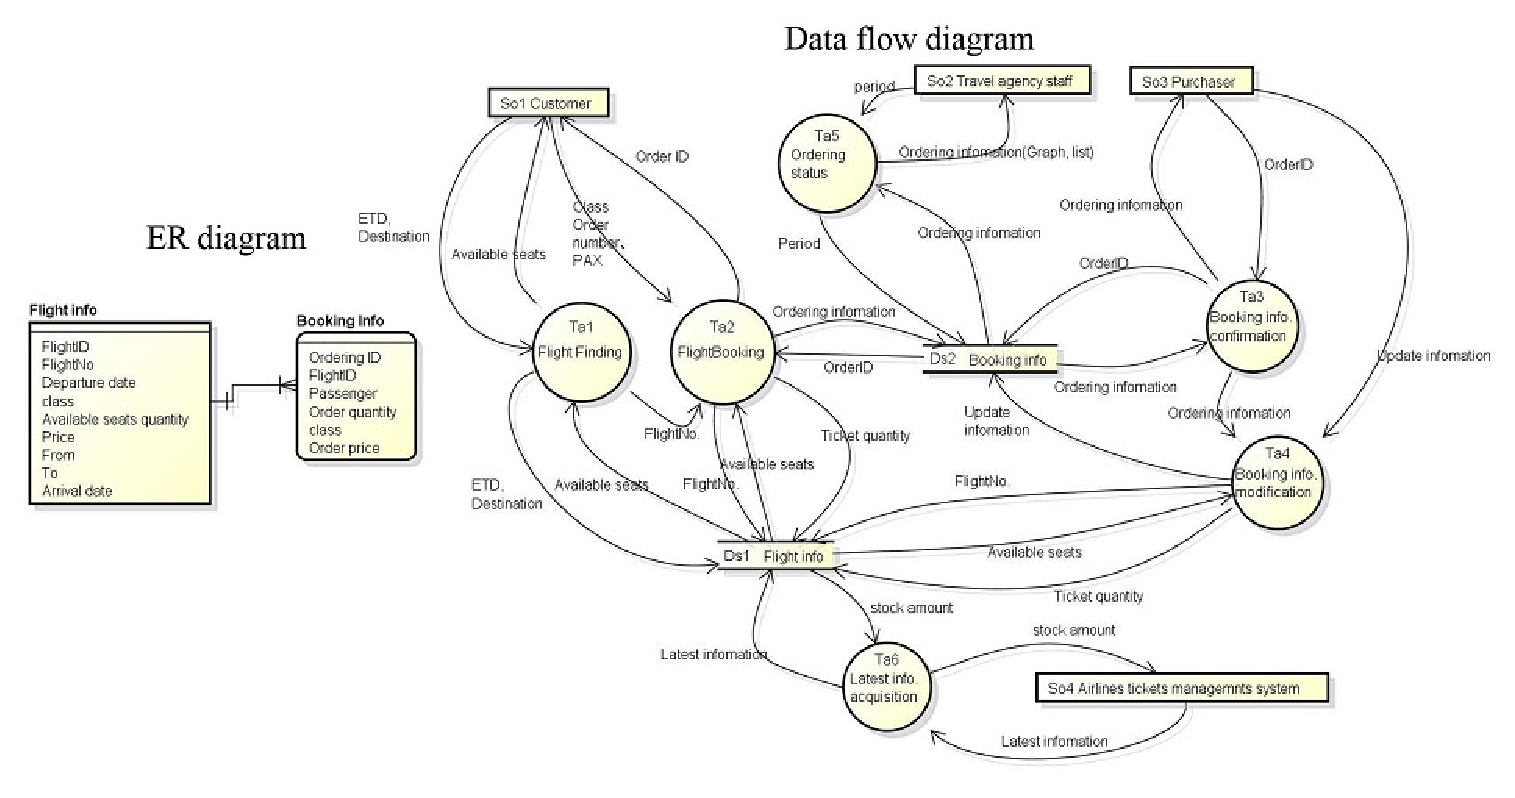
\includegraphics[scale=0.68]{./image/dfdanderd.eps}
\end{center}
\caption{新規フライト予約のデータ設計(一部分)}
\label{fig:DFD}
\end{figure*}

題材となるフライト予約システムの仕様は,本研究の一環として評価実験の際に題材として使っているものである\cite{yumoto2015ICST}\cite{yumoto2016ICST}.
テスト対象の分析と,テストケース設計に関する用語は,国際標準であるISO/IEC/IEEE29119の定義に従い,テスト対象の論理的なサブセットをフィーチャーセットと呼ぶ\cite{ISO29119}.%3-22対応
本論文では,表~\ref{Featurelist}の新規フライト予約を,変更が入ったフィーチャーセットとする.


新規フライト予約からテストケースを抽出するための前提として用意した仕様は,新規フライト予約に関連するDFDとER図(図~\ref{fig:DFD}),CRUD図(表~\ref{CRUD})とする.
DFDに含まれるタスク数 $N$は6,データストア数$M$は2,源泉数$L$は4である.

\begin{table}[t]
\caption{フライト予約システムのフィーチャーセット一覧}
\label{Featurelist}
\begin{center}
\begin{tabular}{l|l}
\hline
テストアイテム&フィーチャーセット
\\
\hline\hline
フライト予約システム&メニュー\\
\cline{2-2}
&ログイン\\
\cline{2-2}
&新規フライト予約\\
\cline{2-2}
&予約変更 \&\\
&キャンセル\\
\cline{2-2}
&予約一覧\\
\cline{2-2}
&予約グラフ\\
\cline{2-2}
&同期処理\\
\hline
\end{tabular}
%\halflineskip
\end{center}
\end{table}

\begin{table}[t]
\caption{フライト予約システムのCRUD図}
\label{CRUD}
\begin{center}
{\footnotesize
\begin{tabular}{p{1.7 cm}|c|p{1.5 cm}||p{1 cm}|p{1cm}}
\hline
フィーチャーセット&\multicolumn{2}{c||}{タスク}&\multicolumn{2}{c}{エンティティ}\\
&\multicolumn{2}{c||}{}&$Ds_1$&$Ds_2$\\
&\multicolumn{2}{c||}{}&Flight info.&Booking info.\\
\cline{4-5}
\hline\hline
新規フライト予約&$Ta_1$&フライト検索&R&\\
\cline{2-5}
&$Ta_2$&フライト登録&RU&C\\
\hline
予約変更&$Ta_3$&予約情報確認&&R\\
%Booking cancellation&&&&\\
\cline{2-5}
キャンセル&$Ta_4$&予約情報修正&RU&UD\\
\hline
\shortstack{予約リスト\\予約グラフ}&$Ta_5$&注文状況&&R\\
\hline
\cline{2-5}
同期処理&$Ta_6$&最新情報取得&CU&\\
\hline
\end{tabular}
}
%\halflineskip
\end{center}
\end{table}%

%-----------

\subsection{ルール1:変更タスクの特定}
テストベースであるDFDに含まれるタスク数$N$は6であるが,変更が入った新規フライト予約の変更タスクは,表~\ref{CRUD}のCRUD図を確認するとフライト検索$Ta_1$とフライト予約$Ta_2$であることがわかる.
図~\ref{fig:DFD}から,$Ta_1$と$Ta_2$の外部入力を確認する.
$Ta_1$は,Customer$So_1$からETDとDestinationを外部入力し,$Ta_2$は,Customer$So_1$からFlightNo,Cl$AS$s,Order number,PAXを外部入力している.

続いて,$Ta_1$と$Ta_2$の内部出力を確認する.
$Ta_1$はFlight info$Ds_1$に対して検索条件を与えているのみで内部入力はしていないため,変更タスク群$P\{Ta\}$からは除外する.
$Ta_2$がFlight info$Ds_1$で$U$,Booking info$Ds_2$で$C$を行っていることが表~\ref{CRUD}から読み取れる.
これらから,拡張CRUD図(表~\ref{ECRUD1})を作る.
表~\ref{ECRUD1}から,ルール1に適合する$Ta_2/Ds_1U$,$Ta_2/Ds_2C$を特定できる.

\begin{table}[t]
\caption{フライト予約システムの中間拡張CRUD図}
\label{ECRUD1}
\begin{center}
\begin{tabular}{c||c|c||c|c|c|c}
\hline
タスク&\multicolumn{2}{c||}{データストア}&\multicolumn{4}{c}{源泉}\\
&$Ds_1$&$Ds_2$&$So_1$&$So_2$&$So_3$&$So_4$\\
\hline\hline
$Ta_1$&&&&&&\\
\hline
$Ta_2$&$U$&$C$&$In$&&&\\
\hline
\end{tabular}
%\halflineskip
\end{center}
\end{table}%

\subsection{ルール2:波及タスクの特定}
ルール2にて波及タスク群$S\{Ta\}$を抽出するために,タスクの外部出力を図~\ref{fig:DFD}のDFDから調べる.
$P\{Ds\}$に含まれる$Ds_1$と$Ds_2$とエッジを持ち,かつ$So$へ出力するタスク群が$S\{Ta\}$候補である.
図~\ref{fig:DFD}では,全てのタスクが$Ds_1$および$Ds_2$からのエッジを持つ.
しかし,$So$への出力に着目すると,$Ta_4$は該当するエッジがないため,$S\{Ta\}$候補には入らない.

$S\{Ta\}$候補のうち、表~\ref{table:3}の○がつく組合せに相当する$Ta_i$が,ルール2で特定したタスクとなる.
本章の例の場合,$P\{Ta\}$での操作は,$C$と$U$であるため,$S\{Ta\}$候補の中で$C$の操作をする$Ta_i$以外は全てルール2で特定したタスクとなる.

これらに該当する$Ta_i$と$Ds$へのCRUD操作,そして$So$への$Out$を追記し,表~\ref{ECRUD2}を完成させる.

\begin{table}[t]
\caption{フライト予約システムの拡張CRUD図}
\label{ECRUD2}
\begin{center}
\begin{tabular}{c||c|c||c|c|c|c}
\hline
タスク&\multicolumn{2}{c||}{データストア}&\multicolumn{4}{c}{源泉}\\
&$Ds_1$&$Ds_2$&$So_1$&$So_2$&$So_3$&$So_4$\\
\hline\hline
$Ta_1$&$R$&&$Out$&&&\\
\hline
$Ta_2$&$RU$&$C$&$InOut$&&&\\
\hline
$Ta_3$&&$R$&&&$Out$&\\
\hline
$Ta_5$&&$R$&&$Out$&&\\
\hline
$Ta_6$&$CU$&&&&&$Out$\\
\hline
\end{tabular}
%\halflineskip
\end{center} 
\end{table}%

\subsection{ルール3:手順 順序組合せテストケースの抽出}
表~\ref{ECRUD2}の拡張 CRUD 図から変更タスクと波及タスクの組合せを抽出する.
抽出した変更タスクと波及タスクの組合せに対して,データストアに対する操作を明記したものは以下のとおりとなる.
\begin{itemize}
\item $Ta_2/Ds_1U  \xrightarrow[Ds_1]{} Ta_1R$\\
\item $Ta_2/Ds_1U  \xrightarrow[Ds_1]{} Ta_2/Ds_1U$\\
\item $Ta_2/Ds_1U  \xrightarrow[Ds_1]{} Ta_6U$\\
\item $Ta_2/Ds_2C  \xrightarrow[Ds_2]{} Ta_3R$\\
\item $Ta_2/Ds_2C  \xrightarrow[Ds_2]{} Ta_5R$\\
\end{itemize}
これらの変更タスクと波及タスクの操作の順序組合せがテストケースとなる.
抽出した順序組合せが持つ入力の条件や出力の特性を仕様から抜き出して論理的テストケースとしてまとめる.
表~\ref{TCLIST2}に論理的テストケースとしてまとめた結果を示す.
\begin{table}[h]
\footnotesize
\caption{順序組合せテストによる論理的テストケース}
\label{TCLIST2}
\begin{center}
%\begin{tabular}{c|p{1 cm}|p{3.5 cm}|p{1.5 cm}}
\begin{tabular}{c|p{3 cm}|p{2.1 cm}}
\multicolumn{3}{l}{新規フライト予約}\\
\hline
No&論理的テストケース&順序組合せ\\
\hline\hline
1&フライト予約後の空き情報問合せによる同一フライトの参照&$Ta_2/Ds_1U  \xrightarrow[Ds_1]{} Ta_1R$\\
\hline
2&フライト予約後の再度同一フライトの予約&$Ta_2/Ds_1U  \xrightarrow[Ds_1]{} Ta_2/Ds_1U$\\
\hline
3&フライト予約後の同期処理によって最新のチケット残数の計算&$Ta_2/Ds_1U  \xrightarrow[Ds_1]{} Ta_6U$\\
\hline
4&既存注文開く画面での予約したフライトの参照&$Ta_2/Ds_2C  \xrightarrow[Ds_2]{} Ta_3R$\\
\hline
5&注文件数グラフ・注文履歴の一覧への新規予約フライト予約の反映&$Ta_2/Ds_2C  \xrightarrow[Ds_2]{} Ta_5R$\\
\hline
\end{tabular}
%\halflineskip
\end{center}
\end{table}

\subsection{順序組合せテストの適用評価} \label{sec:5-2-2}
\begin{figure}[h]
\begin{center}
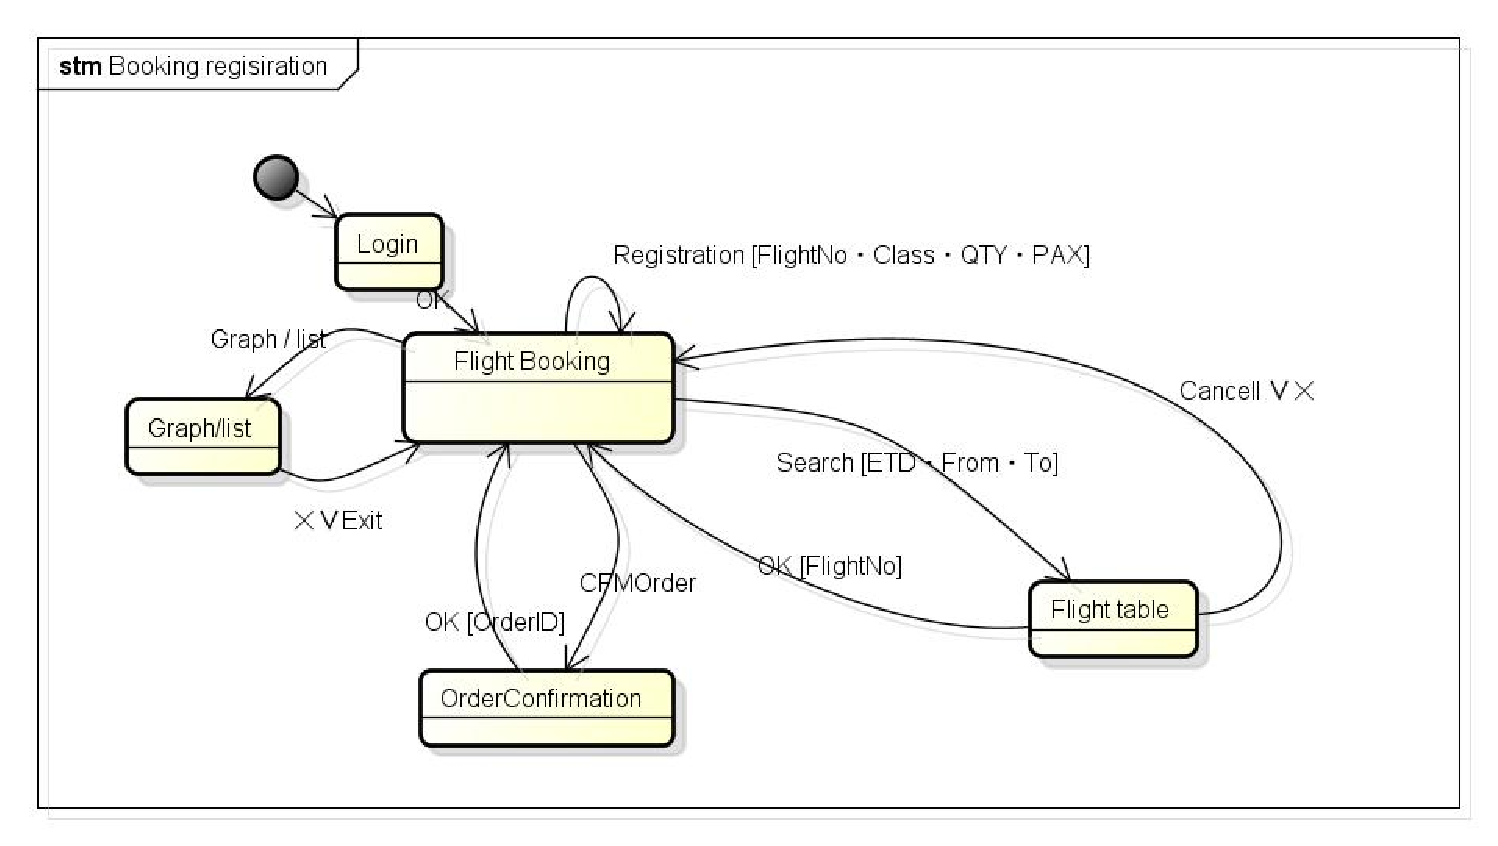
\includegraphics[scale=0.5]{./image/screentransition.eps}
\end{center}
\caption{フライト予約システムの画面遷移図(新規フライト予約)}
\label{fig:STD}
\end{figure}

提案手法で抽出したタスク間の順序組合せと既出の状態を含む$AP$のテストケースを設計する手法である状態遷移テストで,抽出されるテストケースの比較を行う.
状態遷移テストのテストベースとなるフライト予約システムの画面遷移図である図~\ref{fig:STD}を使って,順序組合せが確認できる網羅基準であるS1網羅基準を適用する.
図~\ref{fig:STD}は,適用範囲を合わせるために,4章の適用のためのサブセットである新規フライト予約を行うために必要な画面と隣接する画面遷移に該当する範囲の図となっている.
仕様の詳細度合いは,DFD,ER図,CRUD図と画面遷移図では同等にしている.
それは,画面遷移のイベントでのガード条件に記載したデータがDFDのエッジに記載したデータ,ER図のエンティティの属性と一致していることから確認できる.
S1網羅基準を適用した結果として,表~\ref{tab:STDS1}に28の状態遷移パスを示した。
この表の提案手法(Proposal method)の列には,提案手法で抽出した順序組合せに該当する順序組合せを示した。




S1網羅基準を適用すると28の状態遷移パスとなる.
28の状態遷移パスのうち,対応する提案手法で抽出した順序組合せは,表~\ref{TCLIST2}テストケースNo.1,2,4,5の4つであった.
これらは,本状態遷移図のフライト予約状態での登録イベントを起点にするもののみであった.

\begin{table}[t]
\scriptsize
\centering
  \caption{フライト予約登録の画面遷移図のS1パス一覧}
\begin{tabular}{p{1 em}|p{5 em}|p{9.5 em}|p{5 em}|p{9.5 em}|p{5 em}|p{2 em}}
    No    & 状態    & イベント   & 状態    & イベント& 状態 &提案手法\\
\hline
\hline
    1     & Flight Booking  & Registration [FlightNo・Class・QTY・PAX] & Flight Booking  & Registration [FlightNo・Class・QTY・PAX] & Flight Booking  &  2 \\
\hline
    2     & Flight Booking  & Search [ETD・From・To] & Flight table & Cansell $\lor$× & Flight Booking  &  \\
\hline
    3     & Flight Booking  & Search [ETD・From・To] & Flight table & OK [FlightNo] & Flight Booking  &  \\
\hline
    4     & Flight Booking  & CFMOrder & OrderConfirmation & OK [OrderID] & Flight Booking  &  \\
\hline
    5     & Flight Booking  & Graph & Graph/list & ×$\lor$ Exit & Flight Booking  &  \\
\hline
    6     & Flight Booking  & Registration [FlightNo・Class・QTY・PAX] & Flight Booking  & Search [ETD・From・To] & Flight table & 1 \\
\hline
    7     & Flight Booking  & Registration [FlightNo・Class・QTY・PAX] & Flight Booking  & CFMOrder & OrderConfirmation & 4 \\
\hline
    8     & Flight Booking  & Registration [FlightNo・Class・QTY・PAX] & Flight Booking  & Graph & Graph/list & 5 \\
\hline
    9     & Flight table & Cansell $\lor$× & Flight Booking  & Registration [FlightNo・Class・QTY・PAX] & Flight Booking  &  \\
\hline
    10    & Flight table & OK [FlightNo] & Flight Booking  & Registration [FlightNo・Class・QTY・PAX] & Flight Booking  &  \\
\hline
    11    & Flight table & Cansell $\lor$× & Flight Booking  & Search [ETD・From・To] & Flight table &  \\
\hline
    12    & Flight table & OK [FlightNo] & Flight Booking  & Search [ETD・From・To] & Flight table &  \\
\hline
    13    & Flight table & Cansell $\lor$× & Flight Booking  & CFMOrder & OrderConfirmation &  \\
\hline
    14    & Flight table & OK [FlightNo] & Flight Booking  & CFMOrder & OrderConfirmation &  \\
\hline
    15    & Flight table & Cansell $\lor$× & Flight Booking  & Graph & Graph/list &  \\
\hline
    16    & Flight table & OK [FlightNo] & Flight Booking  & Graph & Graph/list &  \\
\hline
    17    & OrderConfirmation & OK [OrderID] & Flight Booking  & Registration [FlightNo・Class・QTY・PAX] & Flight Booking  &  \\
\hline
    18    & OrderConfirmation & OK [OrderID] & Flight Booking  & Search [ETD・From・To] & Flight table &  \\
\hline
    19    & OrderConfirmation & OK [OrderID] & Flight Booking  & CFMOrder & OrderConfirmation &  \\
\hline
    20    & OrderConfirmation & OK [OrderID] & Flight Booking  & Graph & Graph/list &  \\
\hline
    21    & Graph/list & ×$\lor$ Exit & Flight Booking  & Registration [FlightNo・Class・QTY・PAX] & Flight Booking  &  \\
\hline
    22    & Graph/list & ×$\lor$ Exit & Flight Booking  & Search [ETD・From・To] & Flight table &  \\
\hline
    23    & Graph/list & ×$\lor$ Exit & Flight Booking  & CFMOrder & OrderConfirmation &  \\
\hline
    24    & Graph/list & ×$\lor$ Exit & Flight Booking  & Graph & Graph/list &  \\
\hline
    25    & Login & OK    & Flight Booking  & Registration [FlightNo・Class・QTY・PAX] & Flight Booking  &  \\
\hline
    26    & Login & OK    & Flight Booking  & Search [ETD・From・To] & Flight table &  \\
\hline
    27    & Login & OK    & Flight Booking  & CFMOrder & OrderConfirmation &  \\
\hline
    28    & Login & OK    & Flight Booking  & Graph & Graph/list &  \\
\hline

    \end{tabular}%
  \label{tab:STDS1}%
\end{table}%







順序組合せに該当しない状態遷移パスは,互いのタスクで同一のデータを介して処理をするといったことがない.
例えば,フライト検索をした後にキャンセルをするとフライト予約画面に遷移するパスは,前の処理の結果によって影響を及ぼさない.

S1網羅基準では抽出できないが,本手法によって抽出できたテストケースは,No.3の$Ta_2/Ds_1U  \xrightarrow[Ds_1]{} Ta_6U$である.
このテストケースは,必要なテストケースと考えられる.
適用評価にて利用したテストベースは,変更が入ったフィーチャーセットに焦点を絞ったものである.
この例では,新規フライト予約が該当する。そのため,図5では,新規フライト予約に隣接する画面遷移が,該当するテストベースとなっている.
表~\ref{TCLIST2}のテストケースNo3における波及タスクである$Ta_6U$は,表~\ref{CRUD}から同期処理のタスクであることがわかるが,新規フライト予約とは別のフィーチャーセットに含まれるタスクであり,フライト予約画面と隣接する画面遷移図には現れない.
そのため,S1網羅基準では抽出することができない.
このテストケースを抽出するためにはフィーチャーセットのサイズを大きくする必要があり,そのフィーチャーセットで状態遷移テストを適用するとテストケースの数はさらに爆発する.

\section{まとめ}
本章では,状態遷移を持つソフトウェアにおいて,変更による変更波及がデータベースや外部変数などの保持データを介して生ずる場合のテストに関して,その網羅基準ととしてIDAU法を提案し,順序組合せテストケースを抽出する手法としてIDAU法を提案した.
DFD,ER図、CRUD図をテストベースとして,3つのルールを適用することでテストが必要な順序組合せを抽出できることを説明した.
提案した手法で組合せが抽出できることを確認するため,フライト予約システムの仕様を具体例にして,適用を行った.
最後に従来手法である画面遷移図からS1網羅基準にて抽出した状態遷移パスと提案手法を比較して,テストケース数の削減ができる効果と,S1レベルの画面遷移の網羅では抽出できないテストケースが抽出できる効果を示した.



%%%%%%%%%%%%%%%%%%%%%%%
--------

\begin{table}[t]
\scriptsize
\centering
  \caption{S1 paths in screen transition of flight booking registration}
\begin{tabular}{p{1 em}|p{7 em}|p{10.5 em}|p{7 em}|p{10.5 em}|p{7 em}|p{7 em}}
    No    & State    & Event   & State    & Event    & State    &Proposal Method\\
\hline
\hline
    1     & Flight Booking  & Registration [FlightNo・Class・QTY・PAX] & Flight Booking  & Registration [FlightNo・Class・QTY・PAX] & Flight Booking  &   $Ta2/Ds1U\rightarrow Ta2/Ds1U$ \\
\hline
    2     & Flight Booking  & Search [ETD・From・To] & Flight table & Cansell $\lor$× & Flight Booking  &  \\
\hline
    3     & Flight Booking  & Search [ETD・From・To] & Flight table & OK [FlightNo] & Flight Booking  &  \\
\hline
    4     & Flight Booking  & CFMOrder & OrderConfirmation & OK [OrderID] & Flight Booking  &  \\
\hline
    5     & Flight Booking  & Graph & Graph/list & ×$\lor$ Exit & Flight Booking  &  \\
\hline
    6     & Flight Booking  & Registration [FlightNo・Class・QTY・PAX] & Flight Booking  & Search [ETD・From・To] & Flight table &   $Ta2/Ds1U \rightarrow Ta1R$ \\
\hline
    7     & Flight Booking  & Registration [FlightNo・Class・QTY・PAX] & Flight Booking  & CFMOrder & OrderConfirmation &   $Ta2C\rightarrow Ta3R$ \\
\hline
    8     & Flight Booking  & Registration [FlightNo・Class・QTY・PAX] & Flight Booking  & Graph & Graph/list &   $Ta2C\rightarrow Ta5R$ \\
\hline
    9     & Flight table & Cansell $\lor$× & Flight Booking  & Registration [FlightNo・Class・QTY・PAX] & Flight Booking  &  \\
\hline
    10    & Flight table & OK [FlightNo] & Flight Booking  & Registration [FlightNo・Class・QTY・PAX] & Flight Booking  &  \\
\hline
    11    & Flight table & Cansell $\lor$× & Flight Booking  & Search [ETD・From・To] & Flight table &  \\
\hline
    12    & Flight table & OK [FlightNo] & Flight Booking  & Search [ETD・From・To] & Flight table &  \\
\hline
    13    & Flight table & Cansell $\lor$× & Flight Booking  & CFMOrder & OrderConfirmation &  \\
\hline
    14    & Flight table & OK [FlightNo] & Flight Booking  & CFMOrder & OrderConfirmation &  \\
\hline
    15    & Flight table & Cansell $\lor$× & Flight Booking  & Graph & Graph/list &  \\
\hline
    16    & Flight table & OK [FlightNo] & Flight Booking  & Graph & Graph/list &  \\
\hline
    17    & OrderConfirmation & OK [OrderID] & Flight Booking  & Registration [FlightNo・Class・QTY・PAX] & Flight Booking  &  \\
\hline
    18    & OrderConfirmation & OK [OrderID] & Flight Booking  & Search [ETD・From・To] & Flight table &  \\
\hline
    19    & OrderConfirmation & OK [OrderID] & Flight Booking  & CFMOrder & OrderConfirmation &  \\
\hline
    20    & OrderConfirmation & OK [OrderID] & Flight Booking  & Graph & Graph/list &  \\
\hline
    21    & Graph/list & ×$\lor$ Exit & Flight Booking  & Registration [FlightNo・Class・QTY・PAX] & Flight Booking  &  \\
\hline
    22    & Graph/list & ×$\lor$ Exit & Flight Booking  & Search [ETD・From・To] & Flight table &  \\
\hline
    23    & Graph/list & ×$\lor$ Exit & Flight Booking  & CFMOrder & OrderConfirmation &  \\
\hline
    24    & Graph/list & ×$\lor$ Exit & Flight Booking  & Graph & Graph/list &  \\
\hline
    25    & Login & OK    & Flight Booking  & Registration [FlightNo・Class・QTY・PAX] & Flight Booking  &  \\
\hline
    26    & Login & OK    & Flight Booking  & Search [ETD・From・To] & Flight table &  \\
\hline
    27    & Login & OK    & Flight Booking  & CFMOrder & OrderConfirmation &  \\
\hline
    28    & Login & OK    & Flight Booking  & Graph & Graph/list &  \\
\hline

    \end{tabular}%
  \label{tab:STDS1}%
\end{table}%

%%%%%%%%%%%%%%%%%%%%%%%
\chapter{結論}

本研究では,ソフトウェア開発において,テストケースを作成する工程に投入される人員が、必要なテストケースを網羅的に抽出し,抜け漏れを防止できるようにすることを目的とし,適切な数のテストケースを開発するための手法として,I/Oテストデータパターンと順序組み合わせテストを提案し,その適用評価を行った.

まず,2章では,本研究の対象範囲を明確にするために,対象となるアプリケーションソフトウェア,テストケース設計の種類,テストレベル,テストプロセスを明記した.
そして,ソフトウェアテストの中でも,システムテストレベルでのブラックボックステストを研究の対象にすること,ブラックボックステストのテストケースを開発する活動の中では,テスト分析を対象にすることを述べた,
研究対象の領域で起きている問題として,テスト対象を詳細化する際の分類に対する一貫性が欠如していること,また,機能間の統合に対する問題として,既存の網羅基準を適用するとテストケース数が゙膨大になることを述べた,
これらの問題に対して,テストカテゴリベースドテストというテスト分析手法を基に研究をすすめるため,この手法の概要と,既出の実験結果を説明した.

3章では,テスト分析における詳細化に対する一貫性がの知識を与える前の一貫性のなテスト分析結果,及びばらつきの傾向を適用後の結果との相関をより多くのデータで調べることを目的にした予備実験を行った.
実験はワークショップを通じてグループ単位で2回,個人単位で1回行なった.3回の予備実験を通して,テスト対象を詳細化するときに分類に対する一貫性が欠如していることによるテスト分析結果のばらつきを確認することができた.
また,分類ルールの手法としてテストカテゴリベースドテストの知識を与えることで,テスト条件を特定できる数が増えることが確認できた.仮説として立てた「仕様書には明確に記述がないものは,テストカテゴリのようなガイドを使うことで特定が容易になる」ことが実証できる傾向になった.
ただし,テストカテゴリベースドテストの知識を与えても期待した数のテスト条件を特定できるわけではないことが判明した.
また,業務経歴3年未満の技術者には有効であったが,3年以上の技術者にはあまり効果が出ないことも判明した.

\ref{chap:4}章では,テストカテゴリベースドテストの課題を解決するために,テスト実行時のデータ入出力の要素で分類し網羅的に分析するI/Oテストデータパターンを提案した.
I/Oテストデータパターンの適用評価のために,3章のグループ単位の予備実験の結果を使い,テストカテゴリベースドテストにて分類したテスト条件がI/Oテストデータパターンでどのように分類されるかを確認した.
単一のデータ入出力である,入力調整,出力調整,貯蔵,変換に分類されるテスト条件は,I/Oテストデータパターンで特定できることが確認できた.
一方,サポートと相互作用に分類されるテスト条件は,I/Oテストデータパターンにて分類は可能であるが,単一のデータ入出力で動作するタスクではなく,その後に動作するタスクの出力をテストするためのテスト条件を特定する必要があることを確認できた.
サポートと相互作用で確認するタスクの動作するきっかけをトリガーと呼び,トリガーをテストカテゴリとしてテスト条件を特定するようにした.
最後に,入手した現実の開発プロジェクトのテストケースを使い,I/Oテストデータパターンで特定したテスト条件との比較を試みた.
提案したI/Oテストデータパターンで特定したテスト条件と実プロジェクトで作られるテストケースと比較して,不足しているテスト条件の発見が可能であることが確認できた.

\ref{chap:5}章では,状態遷移を持つソフトウェアにおいて,データベースや外部変数などの保持データを介して影響が生ずる場合のテストに関して,複数回行われるデータの入出力の実行順序に着目した手法である順序組合せテストを提案した.
このテスト手法は,テストカテゴリベースドテストにおける相互作用に分類されるトリガーの他処理への反映に対するテストケースを抽出する手法である.
このテストケースは変更の波及を確認することが目的のテストケースである.
また,変更の波及を確認するための順序組合せテストの網羅基準を定義し,波及全使用法(Impact Data All Used:IDAU)とした.
順序組合せテストは,DFD,ER図、CRUD図をテストベースとして,3つのルールを適用することでテストが必要な順序組合せを抽出できることを説明した.
提案した手法で組合せが抽出できることを確認するため,フライト予約システムの仕様を具体例にして適用を行い,適用可能であることを確認した.
最後に従来手法である画面遷移図からS1網羅基準にて抽出した状態遷移パスと提案手法を比較して,テストケース数の削減ができる効果と,S1レベルの画面遷移の網羅では抽出できないテストケースが抽出できる効果を示した.

提案手法に対する今後の取り組みは2つある.
1つは,適用範囲の明確化である.変更のパターン(タスク内の制御ロジックの変更,新しい要素の追加など)に対して,どこまで適用でき,どこからは適用できないかを明らかにする.

もう1つは,今回の提案手法のツール化である.
実際の開発プロジェクトで扱う規模の大きいデータ設計文書に対して本手法を適用する際には,本手法のルールをツール化するといった方法での適用が必要になる.
これらの準備を行い,実践の場に本手法を適用していく.

%%%%%%%%%%%%%%%%%%%%%%%




\chapter{転記前の部分}
\cite{IEEE610.12-90}
\cite{yumoto2006}
\cite{013}
\cite{Ostrand:1988:CMS:62959.62964}
\cite{Grindal:2007:IPM:1332044.1332085}
\cite{takagi2010concurrent}
\section{はじめに}
ソフトウェアの一部に変更を加えた場合,その変更の波及を探る変更波及解析(Change Impact Analysis)は,実務上の大きな課題である.
産業界において変更にかかる活動は,新規開発よりも大きな割合を占めている.
ゼロから新規にソフトウェアを開発するケースは稀であり,何らかの流用を基に変更を加える開発が主流となっている.
開発方法においてもアジャイルが主流となり,変更の積み重ねによって開発が行われている.

しかし,変更波及を合理的に制御する技術は,ソフトウェア工学とって未完成の分野である\cite{arnold1996software}.
変更の背景は,時代と共に課題を難しくしている.
ソフトウェアの多様化と複雑化,再利用範囲の増大などから変更波及の範囲が拡大し,かつ安易な変更による弊害など課題が山積している.
これらの課題に対してソフトウェア工学は十分な解を提供できていない状況にある\cite{li2013survey}.


本論文では,状態遷移を持つソフトウェアにおいて,変更波及がデータベースや外部変数などの保持データを介して生ずる場合のテストについて考える.
課題の一つは,網羅基準である.データフローテストの全使用法(AU法)\cite{beiz90}を基にして,変更波及のテスト網羅基準を波及全使用法(Impact Data All Used:IDAU)として提案する.
もう一つの課題は,IDAU法を満たす具体的な変更波及のテストケースの抽出方法である.変更波及のテストの設計手法として,順序組合せテストを提案する.
最後に,ここで提案するIDAU法のコストの評価、すなわちテストケースの数を従来技法である状態遷移テストのS1網羅基準と比較をして考察を行い,提案する方法が合理的であることを示す.




\section{変更波及とその解析}
本節では,提案する網羅基準やテスト設計手法の前提となる,システムの構成と変更について定義し,変更波及テストの課題について詳細を示す.




\subsection{変更と変更波及}
$AS$に対して,何らかの変更を加える場合について考える.
変更には,なんらかの意図があり,$AS$が持つ機能の変更であったり,不具合に対する変更や,性能や保守性の改善のためのリファクタリングであったりする.
本論文では,変更の意図については取り扱わず,$AS$の構成要素(タスク,状態,保持データ)に対する具体的な変更について考える.ただし,テスト実行するためには,タスクを動かすことが必要となる.そのため,以降の議論はタスクに焦点を絞る.%1-1対応

ひとつの変更$Q$について考える.
変更$Q$は,タスク群$Ta$のあるタスク$Ta_i$に対して行われたとする.
変更$Q$は,コードの削除や追加を含み,その結果$Ta_i$の版$R$が$R+1$に変更される.
この変更の結果を$Ta^{R}_i$から$Ta^{R+1}_i$とする.

変更$Q$の波及には,3つのケースが考えられる.
\begin{enumerate}
  \item 変更波及が無い場合.(リファクタリングに相当)
  \item 変更波及が他のタスクへ波及しない場合.%3-7対応
  \item 変更波及が他のタスクへ波及する場合.
\end{enumerate}

3.の変更波及は,タスク間の参照が図\ref{fig:fig-2}に示すように状態と保持データに限られるならば,該当する状態や保持データの参照を介した範囲が限られると考えられる.
本論文では,この考え方から波及を受けるタスクを特定し,その合理的なテスト設計について論じる.


%−−−-図2を入れる

\begin{figure}[b]
\begin{center}
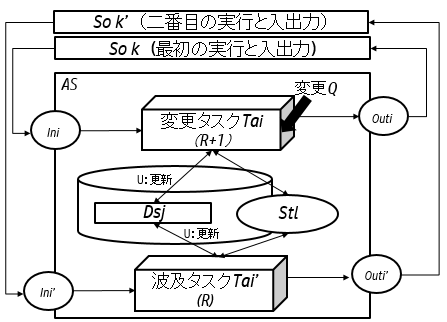
\includegraphics[scale=0.5]{./image/fig-2.png}
\end{center}
\caption{変更タスクと変更波及}
\label{fig:fig-2}
\end{figure}

変更波及,あるいはその解析(Change Impact Analysis)に関する研究は古くから行われている.プロダクトラインやUML図面群を基に依存関係生成モデルを用いて波及解析を行う研究がある\cite{gomaa2005designing,briand2003impact,小谷正行2008}.
タスク内のデータフローを基に変更波及を詳細に解析した研究がある\cite{campbell1990}.
データベースなど保有データを基に変更波及解析を行う研究も行われている\cite{maule2008impact,加藤正恭2011}.
一方,状態と状態遷移はマルコフ過程として実装されているので,過去の状態が未来の状態に影響しない.状態遷移に関する波及解析の研究は見当たらないのはそのためだと推測する.%3-8対応
\cite{LSOF}
\cite{kang1990feature}
\subsection{状態と変更波及のテスト}
変更波及は,保持データを介して波及タスクへ伝達する.状態や状態遷移自身は変更波及に関与しないが,変更波及のテストにおいて与えるデータの順序において状態を考慮する必要が生じる.

保持データの構成について考える.その要素を$Ds=\{Ds_1,Ds_2,\cdots,Ds_j,\cdots,Ds_d\}$とし,変更波及を受ける保持データの要素を$Ds_j$とする.
保持データに対する操作は,データのライフサイクルである「生成:C」「参照:R」「更新:U」「削除:D」を記したCRUD図で定義する.
$Ds_j$を介して変更波及が生ずるのは,変更タスク$Ta_i$において「生成:C」あるいは「更新:U」が行われ,他のタスクで「参照:R」が行われた場合に波及タスクとなる.

保持データのライフサイクル上の「生成:C」「参照:R」「更新:U」「削除:D」などの操作は,無条件に行われるのではなく,操作するタスクの制御フローに沿って行われる.
制御フローは,2階層として捉えることができる.上位の制御フローはタスクの実行順序により決定される大きな制御の流れに相当する.
個々のタスク内の制御フローが下位にあたる.個々のデータ参照実行文はその制御フロー上の条件文で実行が決定される.
条件にはタスクへの入力,保持データ,状態が含まれる.

変更波及を確認するには,変更が波及した保持データを参照するデータフローに沿ってテストを設計することになる.
このデータフローを決定するのは,関係するタスクの実行順序とタスク内の制御フローであり,その制御フローを決定する際に状態が影響する.
状態による制御が想定通りに行われない欠陥は,タスクの実行順序により決定される大きな制御の流れの判断のための状態の確認を,タスク実行のあるタイミングでのみ行っていることが原因となる.%1-2対応による追記
よって,実際のテスト実行においては状態を考慮する必要が生ずる.

\subsection{変更波及テストの網羅基準}

テストにおける網羅基準については,その強度を含め制御フローとデータフローの観点から研究が行われ体系が作られている\cite{beiz90}.
最も弱い網羅基準は制御フローのみに着目した実行文網羅,次が分岐網羅であり,最も強い網羅基準はデータフローを含めた全パス網羅(All Paths)である.%3-9
全パステストは,すべての分岐の積であり現実的には実現不可能のため,全使用法(All Uses)が推奨されている\cite{beiz90}.

変更波及をテストする場合,波及に関与するデータに着目し,そのデータフローテストを行う.
一般的な全使用法は「データを定義したすべての場所から始まり,データを使用するすべての場所に至るまでのパスセグメントを最低限1つを含むテストケース」と定義されている\cite{beiz90}.
この定義を変更タスクと波及タスクとの関係に置き換え「変更タスクにおいてデータの生成および更新があるデータを使用するすべてのタスク(波及タスク)を2つのタスクを実行するまでに経由するルートにかかわらず最低限1つ含むテストケース」とし,波及全使用法とする.

\addtocontents{toc}{\contentsline {chapter}{\numberline {}参考文献}{123}}

% \begin{thebibliography}{9}
  %% 情報処理学会のフォーマットを使用
% \bibliographystyle{ipsjunsrt}
  %% 電子情報通信学会のフォーマット
  \bibliography{mybib1}
  \bibliographystyle{junsrt}
%\bibliographystyle{jplain}

% \bibitem{Cond95}
% Huni,~H., R.~Johnson, and R.~Engel ``A Framework for Network Protocol Software'',
% {\em Proceedings of OOPSLA'95}, pp. 358--369, 1995.
% \end{thebibliography}

%追加した 湯本
%\end{multicols}
\end{document}
